%% 
%% Copyright 2019-2024 Elsevier Ltd
%% 
%% This file is part of the 'CAS Bundle'.
%% --------------------------------------
%% 
%% It may be distributed under the conditions of the LaTeX Project Public
%% License, either version 1.3c of this license or (at your option) any
%% later version.  The latest version of this license is in
%%    http://www.latex-project.org/lppl.txt
%% and version 1.3c or later is part of all distributions of LaTe
%% version 1999/12/01 or later.
%% 
%% The list of all files belonging to the 'CAS Bundle' is
%% given in the file `manifest.txt'.
%% 
%% Template article for cas-dc documentclass for 
%% double column output.

\documentclass[a4paper,fleqn]{cas-dc}

% If the frontmatter runs over more than one page
% use the longmktitle option.

%\documentclass[a4paper,fleqn,longmktitle]{cas-dc}

\usepackage[numbers, compress]{natbib}
%\usepackage[authoryear]{natbib}
%\usepackage[authoryear,longnamesfirst]{natbib}
\usepackage{float}
\usepackage{algorithm}
\usepackage{algpseudocode}

%%%Author macros
\newcommand{\etal}{\emph{et~al.}}
\def\tsc#1{\csdef{#1}{\textsc{\lowercase{#1}}\xspace}}
\tsc{WGM}
\tsc{QE}
%%%

% Theorem environments
\newtheorem{theorem}{Theorem}
\newtheorem{lemma}{Lemma}
\newproof{proof}{Proof}
\newdefinition{definition}{Definition}
\newtheorem{corollary}{Corollary}
\newtheorem{remark}{Remark}

\begin{document}
\let\WriteBookmarks\relax
\def\floatpagepagefraction{1}
\def\textpagefraction{.001}

% Main title of the paper
\title[mode=title]{Joint Horizontal-Vertical Speed Optimization for Energy-Efficient UAV Data Collection}
% Alternative title candidates:
% Energy-Optimal UAV Data Collection via Joint Speed and Altitude Scheduling
% A 3D Distance--Time--Height Framework for Energy-Efficient UAV Data Collection
% Optimal Joint Speed and Altitude Scheduling for Energy-Efficient UAV Data Collection
% joint horizontal-vertical speed optimization (JHVSO) algorithm

% Short title
\shorttitle{}    

% First author
%
% Options: Use if required
% eg: \author[1,3]{Author Name}[type=editor,
%       style=chinese,
%       auid=000,
%       bioid=1,
%       prefix=Sir,
%       orcid=0000-0000-0000-0000,
%       facebook=<facebook id>,
%       twitter=<twitter id>,
%       linkedin=<linkedin id>,
%       gplus=<gplus id>]
\author[2]{Haozhe~Zhang}
\ead{421785689a@gmail.com}
\author[1, 2]{Feng~Shan}[orcid=0000-0001-7398-8265] \cormark[1]
\ead{shanfeng@seu.edu.cn}
\author[1, 2]{Ming~Yang}
\ead{yangming2002@seu.edu.cn}

\address[1]{School of Computer Science and Engineering, Southeast University, Nanjing 211189, Jiangsu, P. R. China}
\address[2]{Jiangsu Key Laboratory of Network and Information Security, Southeast University, Nanjing 211189, Jiangsu, P. R. China}

% Short author
\shortauthors{}  

% Corresponding author text
\cortext[1]{Corresponding author}

% For a title note without a number/mark
%\nonumnote{}

% Here goes the abstract
\begin{abstract}
Unmanned aerial vehicles (UAVs) have emerged as an efficient platform for periodically collecting massive amounts of data from distributed ground nodes (GNs) deployed for environmental and infrastructure monitoring.
Given the limited onboard energy of UAVs, energy-efficient trajectory optimization is critical, yet existing studies often restrict vertical movement or treat height adjustments independently as discrete transitions between horizontal segments.
To capture realistic three-dimensional motion, we adopt a practical 3D flight energy consumption model and jointly optimize the horizontal and vertical speeds.
Moreover, because the ground-to-air communication range varies with flight height, the horizontal and vertical speeds must be jointly optimized to balance communication coverage and flight energy consumption.
Accordingly, we formulate a joint horizontal--vertical speed optimization (JHVSO) problem that simultaneously considers horizontal and vertical motions, height-dependent communication ranges, and the required data collection time of each GN.
We establish key optimality properties by proving that constant-velocity straight-line flight minimizes the energy between two states for a given duration and deriving the pitch-angle-dependent speed that minimizes energy consumption per unit distance during unconstrained flight.
Based on these properties, we develop an Optimal Reached Energy (ORE) dynamic programming algorithm that decomposes the trajectory into gap and task segments, recursively evaluates feasible communication-boundary transition states, and guarantees global optimality over the discretized state space through the non-aftereffect property between successive stages.
Extensive simulations across 34 experimental configurations show that ORE consistently consumes less energy than ASSUME, MSMO, ACO, and a greedy speed--height baseline, reducing energy consumption by up to 14.8\% compared with the greedy speed--height baseline and by up to 5.1\% over the strongest competing baseline, while a case study involving 10 real-world traffic-camera locations further demonstrates its practical applicability.
\end{abstract}
%TODO 摘要中的数据4%太小了，实验部分6.2需要通篇修改，每一个字体都要增加量化的性能提升，并选择亮眼的数字，放到摘要中，替换4%。
%TODO 图片或者表格的caption全部检查一遍，要包括主要核心内容：读者如果仅仅读图和图标题，也能大致了解咱们的方法和技术

% Keywords
\begin{keywords}
Unmanned aerial vehicle \sep Data collection \sep Trajectory optimization \sep Joint speed and altitude scheduling \sep Dynamic programming \sep Energy efficiency
\end{keywords}

\maketitle

%标题
%
% Main text

%%%%%%%%%%%%%%%%%%%%%%%%%%%%%%%%%%%%%%%%%%%%%%%%%%%%%%%%%%%%%%%%%%%%%%%%%%%%%%%%%%
%%%%%%%%%%%%%%%%%%%%%%%%%%%%%%%%%%%%%%%%%%%%%%%%%%%%%%%%%%%%%%%%%%%%%%%%%%%%%%%%%%

\section{Introduction}
\label{sec:intro}

Unmanned aerial vehicles (UAVs) have become an active area of research and have emerged as a pivotal technology for collecting data from distributed ground nodes (GNs)~\cite{lbc, assume, joint, Energy-Efficient-POI, msmo, DroneTank, Flight-Time-Minimization, AoI-Sensitive-Data-Collection, Cooperative-Data-Collection, Data-collection-and-offloading}.
GNs are widely deployed for environmental and infrastructure monitoring in settings such as bridges and railways, water, gas, and oil pipelines, and rivers and coastlines.
These GNs generate massive amounts of data that must be collected efficiently and periodically.
For example, Fig.~(\ref{fig:uav-data-collection-scenario}) illustrates a scenario in which sensors are deployed along a street in a city, and a UAV is dispatched to collect data from them by flying nearby and establishing line-of-sight (LoS) links. 

\begin{figure}
\centering
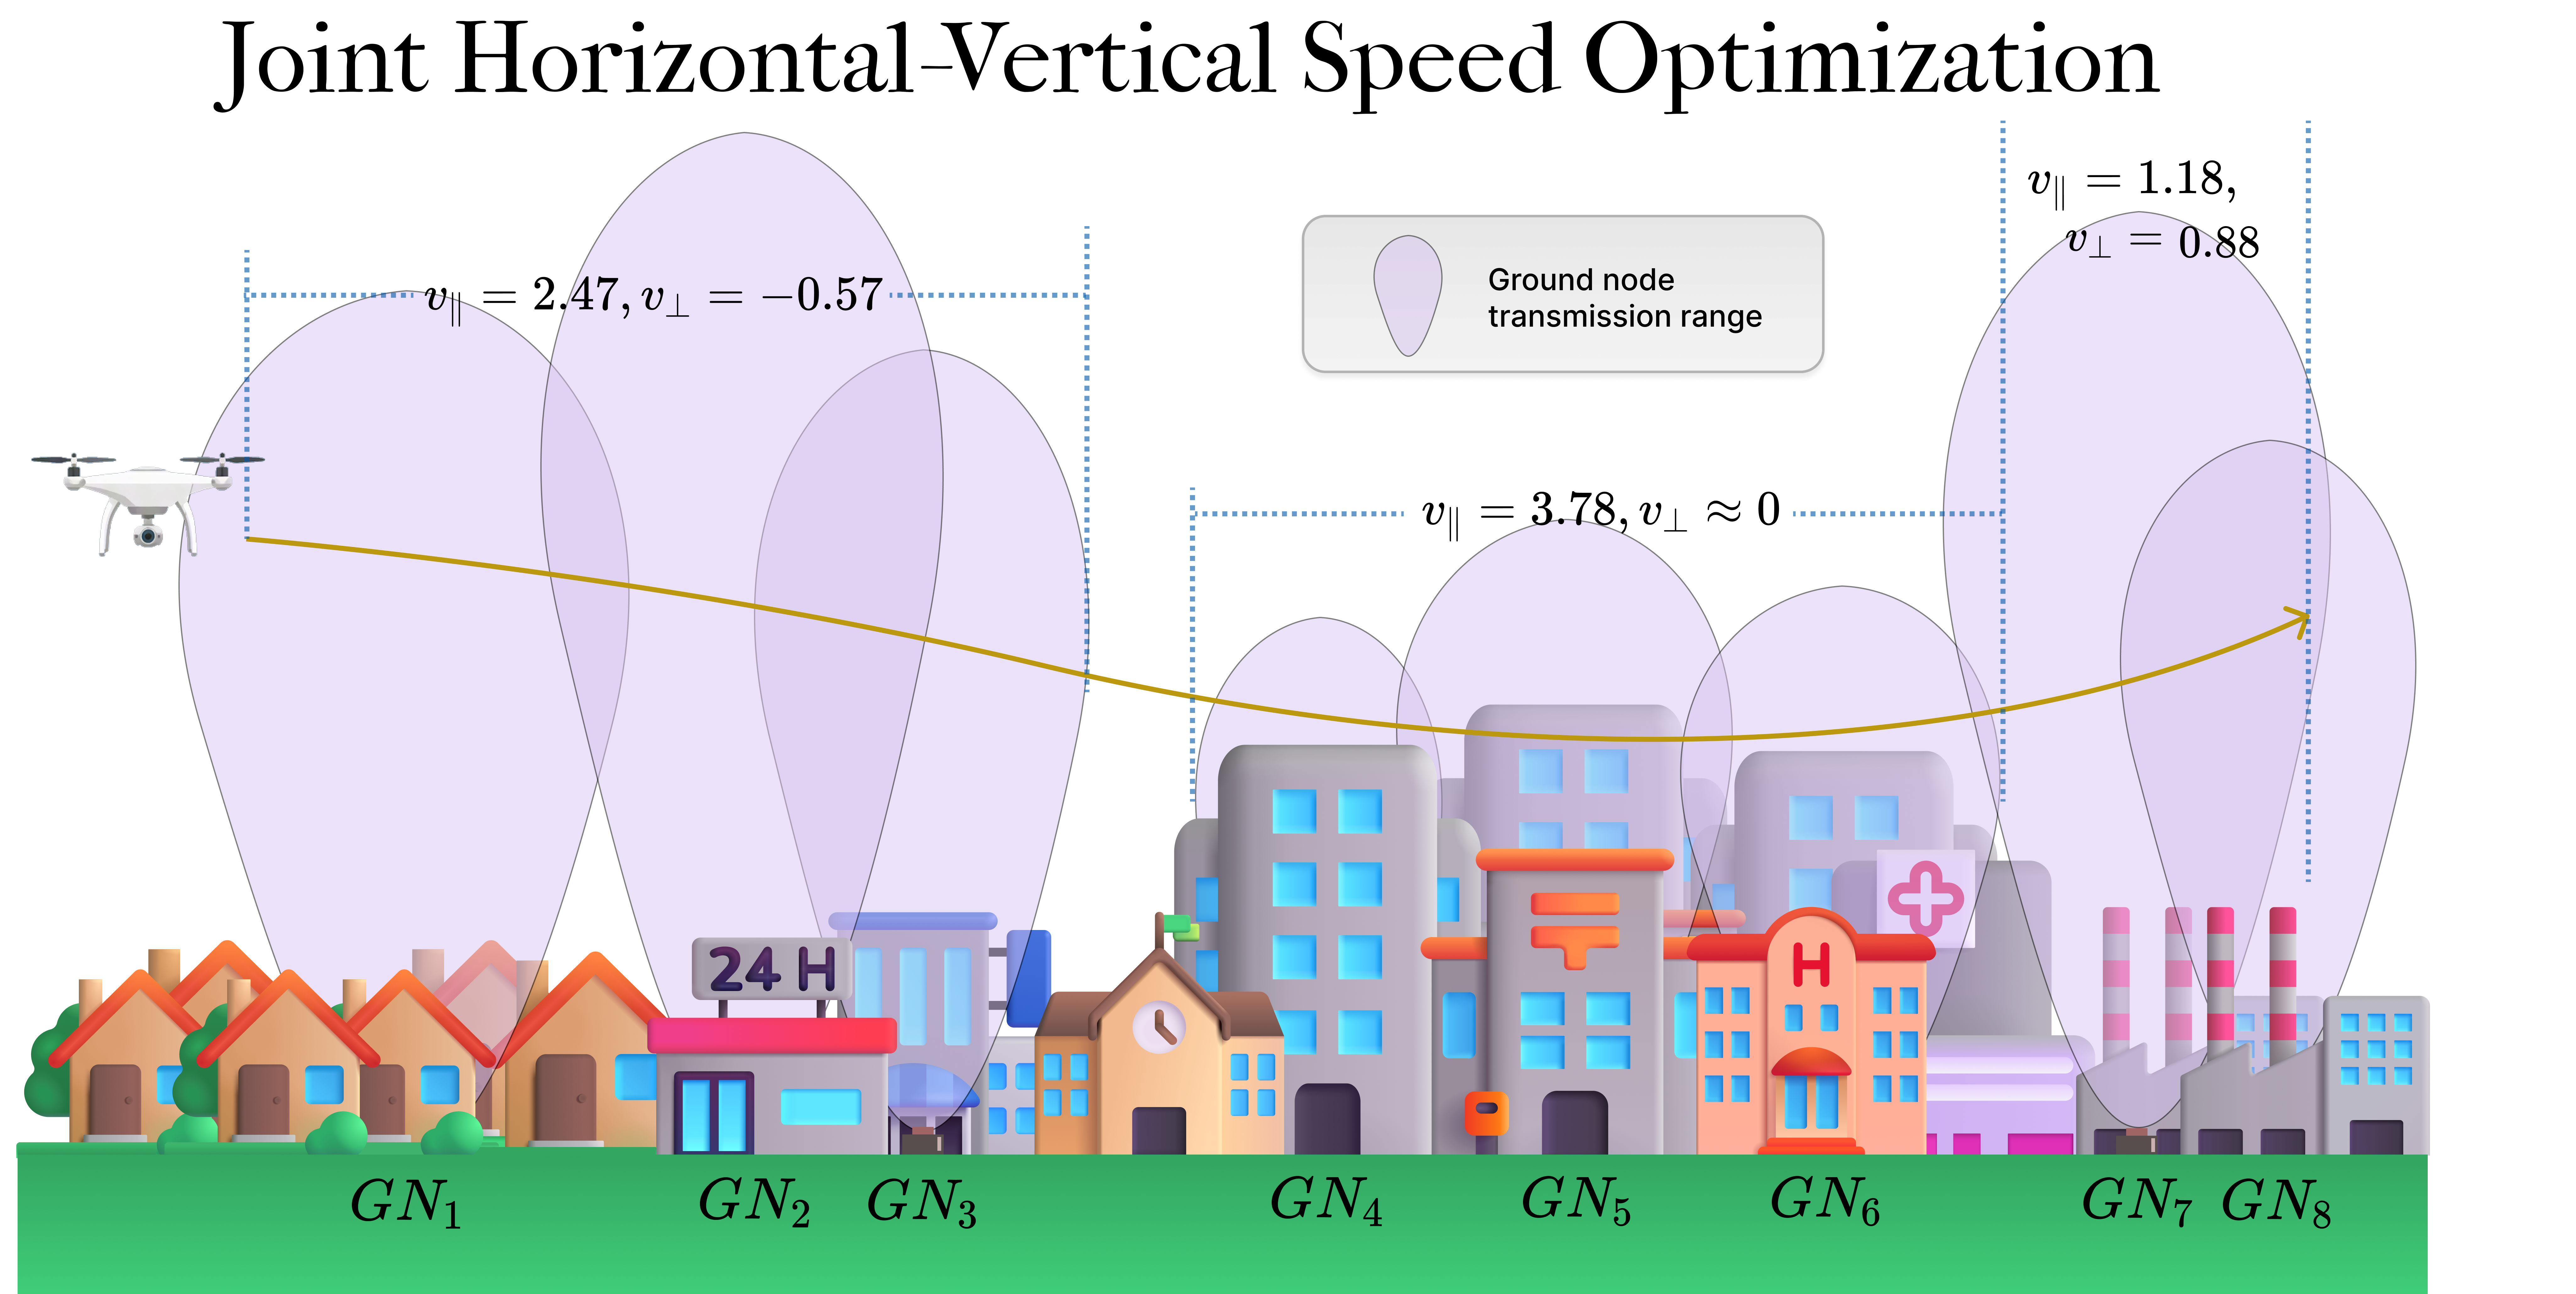
\includegraphics[width = 1\linewidth]{figures/figure1.png}
\caption{UAV-enabled data collection from distributed ground nodes (GNs) along linear infrastructure. A UAV flies along the deployment axis and collects data from each $GN_i$ through an altitude-dependent communication model (shaded cones), within which the UAV must remain for the required collection duration $\tau_i$. The horizontal speed $v_{\parallel}$ and vertical speed $v_{\perp}$ are jointly and continuously optimized so as to minimize the total flight energy while satisfying every GN's collection-time requirement.}
\label{fig:uav-data-collection-scenario}
\end{figure}

Given the inherent energy constraints of UAVs, optimizing flight trajectories to minimize energy consumption is critical~\cite{lbc, assume, joint}.
However, existing studies either concentrate on speed scheduling at a fixed height and restrict the vertical movement of UAVs~\cite{lbc}, or treat vertical movements independently as discrete transitions between horizontal segments~\cite{assume}.
In other words, the UAV's height is adjusted primarily for different horizontal sections rather than treated as a continuous variable in the optimization process~\cite{joint}.
In conclusion, in previous studies, the UAV's vertical movement is often treated independently or as discrete transitions between horizontal segments.

Distinct from previous works, we adopt a practical 3D flight energy consumption model.
Instead of optimizing horizontal speed and height separately, we focus on joint horizontal-vertical speed optimization.
Research has found that instantaneous flight power can be accurately calculated by summing the baseline hovering power with the independent power increments induced by the horizontal and vertical velocity components~\cite{GongHao, PowerConsumptionModel}.

Additionally, this paper assumes that the ground-to-air communication range varies with the UAV's flight height, which is more practical~\cite{assume}.
Although a higher height increases the probability of LoS, it may simultaneously reduce the communication coverage area of the UAV, which influences the level of energy minimization achieved. 
This observation motivates us to carefully optimize the horizontal and vertical speeds jointly to minimize the energy consumption for data collection.

Despite incorporating both the practical 3D flight energy consumption model and joint horizontal-vertical speed optimization, several challenges remain.

\begin{itemize}
\item 
GNs have different data collection volume requirements, which means that the UAV must fly at different speeds within the communication range of each GN to satisfy the required collection time.
Some communication ranges overlap, and the UAV collects data from only one GN at a time; therefore, the UAV must decide when to switch between GNs for data collection.

\item 
With our practical ground-to-air communication model, the communication range varies with height, which means that the UAV must also optimize the vertical component of its velocity.
An inappropriate vertical speed may cause the UAV to fly at an unsuitable height, resulting in a GN communication range that is too small or too large and thereby affecting the speed optimization.
However, the UAV's flight energy consumption is affected by the ascent or descent angle.

\item 
Minimizing the energy cost of data collection during UAV 3D speed optimization presents a further challenge.
On the one hand, the ascent or descent angle directly affects flight energy consumption.
On the other hand, flying faster or slower than a specific speed consumes more energy, as indicated by our practical flight energy consumption model.
How to balance the horizontal and vertical components of the UAV’s velocity while allowing the UAV sufficient time to collect all data at an appropriate height and minimizing flight energy consumption is a challenge.
\end{itemize}


To address this problem, we formulate a joint horizontal-vertical speed optimization problem under a practical 3D flight energy consumption model.
We first investigate its key optimality properties and establish several lemmas and theorems that provide the theoretical foundation for solving the problem.
We then develop an Optimal Reached Energy (ORE) dynamic programming algorithm by decomposing the trajectory into gap and task segments and recursively evaluating feasible transition states.
Finally, we conduct extensive simulations under various settings and a real-world case study to evaluate the energy efficiency and practical applicability of the proposed algorithm.
The major contributions of this paper are summarized as follows:

% contribution outline of the paper
% practical 3D flight energy consumption model
% joint horizontal-vertical speed optimization (JHVSO) problem 
% optimal reached energy (ORE) dynamic programming algorithm 

\begin{itemize}

\item
We formulate a joint horizontal--vertical speed optimization (JHVSO) problem for energy-efficient UAV data collection under a practical 3D flight energy consumption model.
Unlike previous formulations that optimize horizontal speed at a fixed height or schedule height separately, the JHVSO problem jointly considers horizontal and vertical motion, height-dependent communication ranges, and the required data collection time of each GN.

\item
We investigate the key optimality properties of the JHVSO problem and establish several lemmas and theorems that provide its theoretical foundation.
By exploiting the strict convexity of the horizontal and vertical flight energy functions, we prove that constant-velocity straight-line flight minimizes the energy between two states for a given duration.
We also derive the pitch-angle-dependent speed that minimizes the energy consumption per unit distance during unconstrained flight.

\item
We develop an Optimal Reached Energy (ORE) dynamic programming algorithm to solve the JHVSO problem.
By decomposing the UAV trajectory into gap and task segments, recursively evaluating feasible communication-boundary transition states, and establishing the non-aftereffect property between successive stages, the algorithm obtains the optimal local transition costs and \textbf{guarantees the global optimality} of the resulting solution over the discretized state space.

\item
We conduct extensive simulations under varying channel conditions, task durations, node densities, and inter-node distances to evaluate the proposed ORE algorithm.
The results show that the proposed JHVSO method consistently consumes less energy than ASSUME, MSMO, ACO, and a greedy speed--height baseline, achieving an energy reduction of up to approximately 16.8\% compared with the greedy speed--height baseline and by up to 5.8\% over the strongest competing baseline.
A case study involving 10 real-world traffic-camera locations further demonstrates its practical applicability.

\end{itemize}  

The remainder of this paper is organized as follows.
Section~\ref{sec:relatedworks} reviews the related works on energy-efficient UAV data collection and trajectory optimization.
Section~\ref{sec:systemmodel} introduces the system model and formulates the JHVSO problem.
Section~\ref{sec:problemanalysis} analyzes the problem and establishes the optimality properties required for its solution.
Section~\ref{sec:algorithm} presents the proposed ORE dynamic programming algorithm.
Section~\ref{sec:simulation} evaluates its performance through extensive simulations and a real-world case study.
Finally, Section~\ref{sec:conclusion} concludes the paper, and Appendices~\ref{pro:Lemma ver}--\ref{pro:Theorem optimal-range-speed} provide the relevant proofs.

%%%%%%%%%%%%%%%%%%%%%%%%%%%%%%%%%%%%%%%%%%%%%%%%%%%%%%%%%%%%%%%%%%%%%%%%%%%%%%%%%%


\section{Related Works}
\label{sec:relatedworks}
This section reviews speed scheduling for UAV data collection and the flight energy consumption models adopted in this work.

\subsection{Speed Scheduling at a Fixed Altitude}

UAV-aided data-collection from ground nodes (GNs) has been extensively studied, though largely with optimization targets other than flight energy.
Gong \etal~\cite{Flight-Time-Minimization} minimize the mission completion time; Gao \etal~\cite{AoI-Sensitive-Data-Collection} and Wang \etal~\cite{Cooperative-Data-Collection} minimize the age of information of the collected data; Chang \etal~\cite{Data-collection-and-offloading} plan the discrete visiting order of GNs jointly with battery-swapping decisions; and Ning \etal~\cite{Wireless-powered-IOT} integrate data acquisition with wireless power transfer.
In these designs, the flight speed is fixed as a constant or treated merely as a feasibility constraint, leaving the energy-saving potential of speed scheduling unexploited.
The idea of trading service rate for energy under deadline constraints dates back to the energy-efficient transmission scheduling of Zafer and Modiano~\cite{A-calculus-Approach}, where the convexity of the power-rate function implies constant-rate optimality on cumulative data-time diagrams.
UAV speed scheduling exploits the same mathematical structure via the convexity of the propulsion power-speed function.
For UAV data collection, Xiong and Shan~\cite{DroneTank} jointly planned the UAV flight and the sensors' data transmission under energy constraints in DroneTank, and Shan \etal~\cite{lbc} derived the energy-optimal speed profile as a shortest path on a distance-time diagram with the looking-before-crossing (LbC) algorithm.
Ye \etal~\cite{offspeeding} further established a provably optimal offline speed scheduler, Offspeeding, for UAV-assisted edge computing with per-task deadlines, by exploiting the convexity of a practical flight energy consumption model; the idea was later generalized to arbitrary point-of-interest visiting topologies by Shan \etal~\cite{Energy-Efficient-POI} and recently coupled with battery swapping in UAV-enabled mobile edge computing by Ye \etal~\cite{Optimal-Flight-Speed-Scheduling-and-Battery-Swapping}.
Nevertheless, these works confine the UAV to a fixed altitude and adopt energy consumption models accounting for horizontal motion only, ignoring the vertical dimension and the altitude-dependent quality of ground-to-air channels.

\subsection{Speed Scheduling with a Variable Altitude}

When the flight altitude enters the decision space, its coupling with speed substantially complicates the scheduling problem.
Early studies, e.g., Mozaffari \etal~\cite{Mobile-UAVs-for-IoT}, optimized the UAV position or altitude for communication coverage and energy efficiency, yet without scheduling the flight speed.
Closer to our problem, Huang \etal~\cite{assume} jointly schedule altitude and speed for energy-minimal data collection in ASSUME, where vertical movement is modeled as discrete transitions between horizontal flight segments; Wang \etal~\cite{joint} further address unknown visiting orders through ant-colony optimization in JUSAS, at the cost of high computational overhead and without global optimality guarantees.
Towards continuous three-dimensional motion, Sun \etal~\cite{Matrix-Based-Evolutionary-Computation} parameterized the UAV trajectory with Bézier curves and optimized the control points via matrix-based differential evolution over 3D terrain; Ding \etal~\cite{3D-Trajectory-and-Frequency-Band} formulated joint 3D trajectory design, node association, and resource allocation as a (constrained) Markov decision process solved by deep reinforcement learning; and Hoang \etal~\cite{Adaptive-3D-Placement} studied adaptive 3D placement of UAV-mounted base stations in the same spirit.
These works free the vertical dimension, but they either superpose the horizontal and vertical propulsion power in an additive, decoupled manner, or rely on heuristic and learning-based solvers that admit no global optimality guarantee.

\subsection{Flight Energy Consumption Models of Multi-Rotor UAVs}

The credibility of energy-oriented scheduling rests on the underlying flight energy consumption model, which falls into three categories.
Distance-related models account energy by the traveled distance and the number of turns, as in Piao \etal~\cite{Automating} and Modares \etal~\cite{UB-ANC-planner}, whereas duration-related models multiply a constant power by the flight time, as in Ko and Gau~\cite{UAV-Velocity-Function-Design}.
Speed-related models instead capture the fact that the propulsion power is a convex function of the flight speed.
Zeng \etal~\cite{Rotary-Wing-UAV} derived the now-standard analytical model for rotary-wing UAVs, decomposing the power into blade-profile, induced, and parasite components, and Morbidi \etal~\cite{Minimum-energy-path-generation} reached a consistent model from the electrical dynamics of brushless DC motors.
Building on this line, Gong \etal~\cite{GongHao} extended the flight energy consumption model to 3D flight by summing the hovering power with independent increments induced by the horizontal and vertical velocity components, and Liu \etal~\cite{PowerConsumptionModel} further characterized the vertical flight power from actuator-disk theory.
Such speed-related models have been widely adopted in recent UAV-assisted edge computing and trajectory designs~\cite{Safe-and-Energy-Efficient-Trajectory, Energy-Efficient-UAV-Assisted-MEC}).
However, existing 3D extensions typically schedule the two dimensions independently (e.g., as discrete altitude transitions). In contrast, our formulation retains the additive instantaneous-power form of~\cite{GongHao, PowerConsumptionModel} but jointly optimizes the two speed components through the flight pitch angle, as detailed in Section 3.2.

\subsection{Communication Models}

The communication range of a GN served by a UAV is inherently altitude-dependent.
Al-Hourani \etal~\cite{CommunicationModel} derived the optimal altitude of a low-altitude platform that maximizes the coverage radius under a probabilistic line-of-sight (LoS) model, which has become the foundation of altitude-dependent coverage analyses, including the ground-to-air channel model adopted in this work.
In UAV-enabled sensor data collection, the wake-up and communication radius is commonly determined by a signal-to-noise ratio threshold over the ground-to-air link, as in Zhan \etal~\cite{Energy-efficient-data-collection}, and can be further shaped by jointly optimizing the altitude and the antenna beamwidth, as shown by Choi and Lee~\cite{Altitude-and-beamwidth}.
Recent field measurements have revealed additional fine-grained effects: Zhang \etal~\cite{Directivity-Aware-Link-Model} showed that the altitude-induced misalignment of antenna radiation patterns degrades ground-to-air LoRa links, and proposed a directivity-aware annulus link model; Huang \etal~\cite{AIM} incorporated the angle of radiation into relay deployment for 3D connectivity; and Li \etal~\cite{Poisson-Delaunay} characterized the LoS/NLoS probability and coverage statistics of air-ground networks via stochastic-geometry analyses.
This altitude dependence couples the communication opportunity with the vertical motion of the UAV, and hence with its speed scheduling—exactly the coupling exploited in this work.

In summary, while existing research has made significant strides in UAV trajectory planning and energy-efficient speed control, critical gaps remain.
Most current literature either relies on overly simplified flight energy consumption models that neglect the coupled effects of altitude and flight dynamics, or employs heuristic-based algorithms that fail to guarantee global optimality in complex scenarios.
Furthermore, few studies have adequately addressed the joint scheduling of flight speed and altitude as a unified sequential decision process.
To address these deficiencies, this paper moves beyond static or decoupled optimization frameworks.
We propose a rigorous \textit{JHVSO} (Joint Horizontal-Vertical Speed Optimization) model that integrates sophisticated aerodynamic power consumption characteristics.
By leveraging the theoretical properties of the power function and the non-aftereffect nature of multi-stage transitions, we formulate a dynamic programming approach that systematically identifies the global energy-optimal trajectory, providing a more robust and efficient solution for UAV data collection missions.

%%%%%%%%%%%%%%%%%%%%%%%%%%%%%%%%%%%%%%%%%%%%%%%%%%%%%%%%%%%%%%%%%%%%%%%%%%%%%%%%%%
%%%%%%%%%%%%%%%%%%%%%%%%%%%%%%%%%%%%%%%%%%%%%%%%%%%%%%%%%%%%%%%%%%%%%%%%%%%%%%%%%%



\section{System define and problem formulation}
\label{sec:systemmodel}
 
\subsection{Ground-to-Air Communication Model}

We consider a set of ground nodes (GNs) denoted by $\mathcal{N} = \{1, 2, \dots, n\}$, distributed along a pre-defined flight mission path,  such as bridges and railways, water, gas, and oil pipelines, and rivers and coastlines. 
Each  $GN_i \ ,\ i\in \mathcal{N}$ is located at a fixed position and has a specific volume of data to be collected by the UAV.
The smaller the index of the $GN$ means closer to the start point of the flight path.

Following the practical ground-to-air communication model established in~\cite{CommunicationModel}, the communication range of a $GN$ is determined by the two-dimensional distance between the $GN$ and the UAV. 
Let $(r_{i},h_{i})$ denote the relative horizontal and vertical distance of UAV from certain ground node $GN_i$.
The UAV can establish a reliable communication link with $GN_i$ only when the path loss caused by the distance between them $PL_i(r_i,h_i)$ is within threshold $PL^{max}_i$.
Specifically, the condition for data transmission is given by:
$$PL_i(r_i,h_i) \leq PL^{max}_i, $$ 
where the threshold $PL^{max}_i$ of certain $GN_i$ is determined by the ground node itself and given in advancing. 
The connection between UAV and the GN would loss, when the path loss exceeds $PL^{max}_i$ for $GN_i$. 

\begin{multline}
    PL_i(r_i,h_i)
    =\frac{\mu_{LoS}-\mu_{NLoS}}
    {1+a \exp(-b[\frac{180}{\pi}\arctan(\frac{h_{i}}{r_{i}})-a])} \\
    +10 \log(h_{i}^2+r_{i}^2)+M
    \label{equ:PL}
\end{multline}

Eq.~(\ref{equ:PL}) gives the expected path loss under the probabilistic line-of-sight (LoS) model~\cite{CommunicationModel}, where $\mu_{LoS}$ and $\mu_{NLoS}$ are the mean excess losses of LoS and non-LoS links, and $a$ and $b$ are environment-dependent parameters.
The constant $M$ collects the carrier-frequency and free-space propagation factors together with the NLoS excess loss:
\begin{equation}
    M=20\log f+20\log\left(\frac{4\pi}{c}\right)+\mu_{NLoS},
    \label{equ:M}
\end{equation}
where $f$ is the carrier frequency and $c$ is the speed of light.

The key angular variable is the link elevation angle $\theta_i=\frac{180}{\pi}\arctan(h_i/r_i)$ (in degrees), measured between the GN--UAV line and the horizontal plane.
It determines the LoS probability $P_{LoS}(\theta_i)=1/(1+a\exp(-b[\theta_i-a]))$: a larger $\theta_i$ increases the LoS probability and thus reduces the expected excess loss when $\mu_{LoS}<\mu_{NLoS}$.
However, at a fixed horizontal distance, increasing altitude also lengthens the slant range $d_i=\sqrt{h_i^2+r_i^2}$ and increases the free-space loss.
These competing effects determine the altitude-dependent communication region defined by $PL_i(r_i,h_i)\leq PL_i^{max}$, as illustrated in Fig.~(\ref{fig:communication_range}).

To model the data upload, we characterize each $GN_i$ by a nominal SINR $\gamma_i$, which is a per-node design parameter given in advance---like the path-loss threshold $PL_i^{max}$---rather than the instantaneous, position-dependent SINR experienced by the UAV. Letting $B$ denote the channel bandwidth, the achievable rate of the link is evaluated at this nominal SINR through the Shannon capacity:
\begin{equation}
    \bar{R}_i = B\log_2(1+\gamma_i). \label{equ:const_rate}
\end{equation}
Each $GN_i$ therefore uploads data at the constant rate $\bar{R}_i$ throughout the collection phase, which yields the deterministic collection duration $\tau_i = D_i/\bar{R}_i$.

\begin{figure}[]
  \centering
   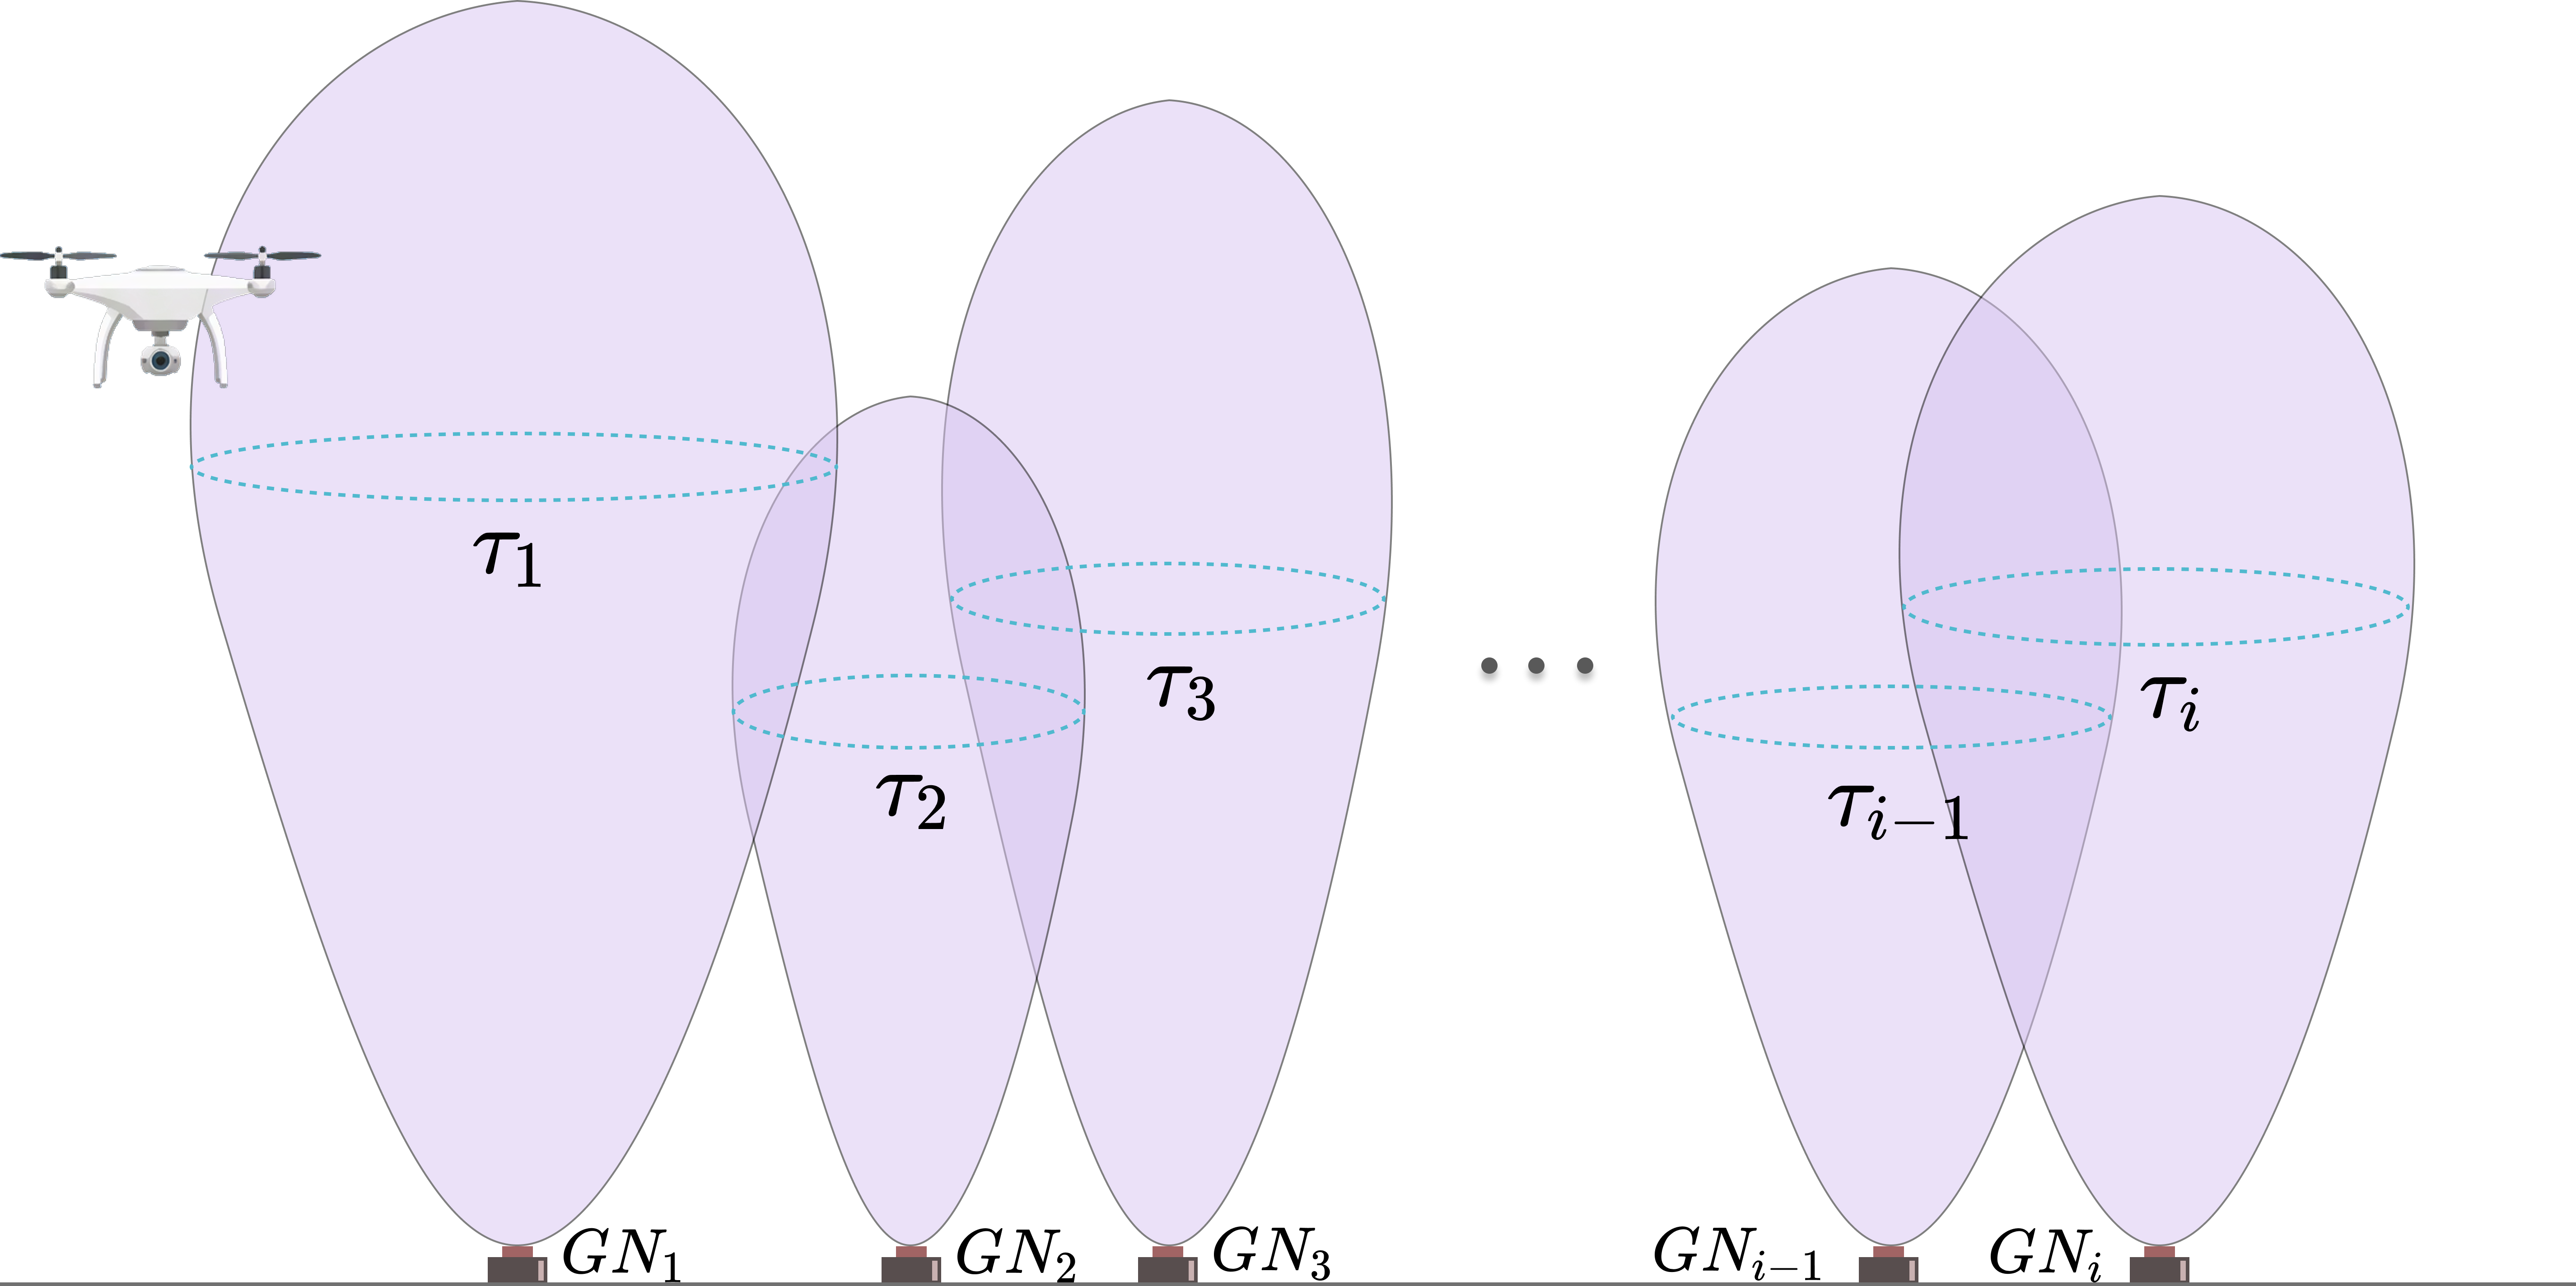
\includegraphics[width = 1\linewidth]{figures/gn-communication-range-3d.png}
    \caption{Altitude-dependent communication regions defined by Eq.~(\ref{equ:PL}) and Eq.~(\ref{equ:M}).
    The UAV must remain within the region of $GN_i$ for the required data collection duration $\tau_i = D_i/\bar{R}_i$, where $D_i$ is the data volume of $GN_i$ and $\bar{R}_i = B\log_2(1+\gamma_i)$ is the constant achievable rate.}\label{fig:communication_range}
\end{figure}

The link elevation angle differs from the UAV's flight-path angle, which describes the direction of its velocity.
Horizontal and vertical speed decisions change $r_i$ and $h_i$ over time, thereby changing both $\theta_i$ and $d_i$ and determining how long the UAV remains within each GN's communication region.
This geometric dependence couples speed and altitude scheduling with the required data collection duration.

\subsection{Flight Energy Consumption Model}

To optimize the UAV's horizontal and vertical speeds for energy-efficient data collection, we first model its propulsion power as a function of these two velocity components.
Following~\cite{GongHao}, we express the total power as the hovering power plus the increments associated with horizontal and vertical motion.

\begin{figure}[]
  \centering
   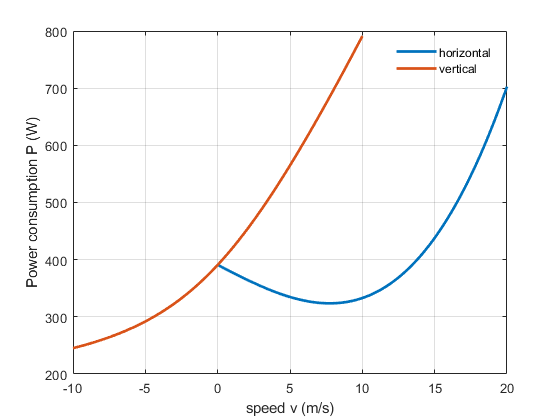
\includegraphics[width = 0.8\linewidth]{figures/uav-power-vs-velocity.png}
    \caption{Horizontal and vertical propulsion power functions used in the simulations.
    The horizontal power in Eq.~(\ref{equ:h_2}), modeled by a cubic polynomial fitted to flight-test measurements, initially decreases and then increases with horizontal speed, reaching a minimum at an intermediate speed.
    The vertical power in Eq.~(\ref{equ:v_1}) increases monotonically with the climb rate.
    Both functions yield the same hovering power, $P_{mh} = 390.95\,\mathrm{W}$, at zero speed.}
\end{figure}

Let $V_{total}$ denote the total (resultant) flight speed and $\gamma$ the flight pitch angle, defined as the angle between the velocity vector and the horizontal plane. The horizontal and vertical velocity components are related to $V_{total}$ and $\gamma$ by
\[
    V_{\parallel} = V_{total}\cos\gamma, \qquad V_{\perp} = V_{total}\sin\gamma.
\]

\begin{equation}
    P_{total}(V_{total}) = P_{mh} + \Delta P_{\parallel}(V_{\parallel}) + \Delta P_{\perp}(V_{\perp}),
    \label{equ:e_1}
\end{equation}

In Eq.~(\ref{equ:e_1}), $P_{mh}$ denotes the hovering power, while $\Delta P_{\parallel}(V_{\parallel})$ and $\Delta P_{\perp}(V_{\perp})$ denote the power increments associated with horizontal and vertical motion, respectively.
This additive model evaluates the two contributions separately to obtain the instantaneous propulsion power during three-dimensional flight.

\textbf{For the horizontal component}, we adopt the analytical propulsion power model in~\cite{GongHao}:

\begin{align}
    &P_{\parallel} = P_{mh}+ \frac{3}{8}\sqrt{n}\delta\sqrt{\frac{W\rho A}{C_{T}}}s||V_{\parallel}||^2+P_{in}
    \nonumber
    \\ &\left[\left(\sqrt{1+\frac{||V_{\parallel}||^4}{4v_0^4}}-\frac{||V_{\parallel}||^2}{2v_0^2}\right)^{1/2}-1\right]+\frac{n}{2}S_{FP\parallel \cdot \rho} ||V_{\parallel}||^3
    \label{equ:h_1}
\end{align}

$$P_{in}\triangleq 1.11 \frac{W^{3/2}}{\sqrt{2n\rho A}}$$

Here, $W$ is the UAV weight, $n$ is the number of rotors, $\rho$ is the air density, and $A$ is the rotor disc area.
The parameters $\delta$, $s$, $C_T$, and $S_{FP\parallel}$ denote the profile drag coefficient, rotor solidity, thrust coefficient, and equivalent flat-plate area, respectively, while $v_0$ is the mean induced velocity in hover.

To simplify platform-specific calibration and numerical evaluation, we use a cubic approximation in the simulations:

\begin{equation}
    P_{\parallel} = c_1 v_{\parallel}^3 + c_2 v_{\parallel}^2 + c_3 v_{\parallel} + P_{mh}\label{equ:h_2}
\end{equation}

The coefficients $c_1$, $c_2$, and $c_3$ are fitted to the flight-test measurements reported in~\cite{assume}, with their values given in Section~\ref{sec:simulation}.
The constant term $P_{mh}$ ensures that both models yield the same power at zero speed.
The fitted model captures the decrease and subsequent increase of horizontal power with speed, and its convexity over the operating range is established below.

\textbf{For the vertical component}, we adopt the steady-state propulsion power model in~\cite{PowerConsumptionModel}.
Under constant-speed vertical flight, rotor thrust balances the UAV weight, and the required power comprises a velocity-dependent induced term and a constant blade-profile term:

\begin{equation}
    P_{\perp} = k_1 mg \left[\frac{V_{\perp}}{2}+\sqrt{\left(\frac{V_{\perp}}{2}\right)^2+\frac{mg}{k_2^2}}\right] + c_1(mg)^{3/2}
    \label{equ:v_1}
\end{equation}

Here, $V_{\perp}$ is the vertical velocity, $m$ is the UAV mass, and $g$ is the gravitational acceleration.
The coefficient $k_1$ corrects for non-uniform rotor inflow, $k_2$ characterizes the induced-flow contribution, and $c_1$ accounts for blade-profile power.
The first term describes the power required to generate thrust, while $c_1(mg)^{3/2}$ represents the power needed to overcome blade drag.
Parasite power is neglected at the moderate vertical speeds considered here.

The parameters $k_1$ and $c_1$ are adopted from~\cite{PowerConsumptionModel}, while $k_2$ and $mg$ are calibrated to approximately match the horizontal model's hovering power, with their values given in Section~\ref{sec:simulation}.

\begin{lemma}[Convexity of the vertical power component]
    \label{lem:ver}
    For any platform parameters $k_1 > 0$, $k_2 > 0$, $c_1 \geq 0$ and weight $mg > 0$, the vertical power function Eq.~(\ref{equ:v_1}) is strictly convex.
\end{lemma}

\begin{proof}
    See Appendix~\ref{pro:Lemma ver} \qed
\end{proof}

\begin{lemma}[Convexity of the horizontal power component]
    \label{lem:hor}
     Write Eq.~(\ref{equ:h_1}) as $P_\parallel(v) = c_1v^3 + c_2v^2 + P_{in}\cdot f(v) + P_{mh}$, where $c_1$ and $c_2$ denote the (positive) coefficients of the parasite terms and blade-profile, $P_{in} > 0$ is the induced-power constant, and $f(v) = [\sqrt{(1 + (v^2/2v_0^2)^2)} - v^2/2v_0^2]^{1/2} - 1$ is the induced-power increment with the mean hover induced velocity $v_0 > 0$.
     Then Eq.~(\ref{equ:h_1}) is strictly convex on $v \geq 0$ whenever $4c_2v_0^2 > P_{in}$, a condition satisfied by conventional multi-rotor configurations, including the platform parameters reported in~\cite{GongHao}.
\end{lemma}

\begin{proof}
    See Appendix~\ref{pro:Lemma hor} \qed
\end{proof}

The strict convexity of the two power components supports the constant-speed optimality results developed in Section~\ref{sec:problemanalysis}.
For the polynomial model in Eq.~(\ref{equ:h_2}), this property can be assessed through its second derivative, $P_\parallel''(v)=6c_1v+2c_2$.
With the parameter values used in Section~\ref{sec:simulation}, this derivative remains positive over the operating speed range, allowing the fitted model to retain the convexity required by the analysis.
For other UAV platforms, the applicability of these results should be assessed using the corresponding model parameters and operating range, together with the remaining assumptions of the formulation.


\subsection{Problem Definition}
\label{subsection:problem}

Let the UAV trajectory be denoted by $q(t) = (d(t), h(t))$, where $d(t)$ and $h(t)$ are the horizontal position along the mission path and the flight altitude at time t, respectively, and let $v_\parallel(t) = \dot{d}(t)$ and $v_\perp(t) = \dot{h}(t)$ be the corresponding velocity components.
Let $v_\parallel \in [0, V_{\parallel}^{max}]$, $|v_\perp| \leq V_{\perp}^{max}$ be the speed limits imposed by hardwares.
By Eq.~(\ref{equ:PL}), each $GN_i$ is associated with an altitude-dependent communication region in the $(d, h)$ plane, obtained from $PL(r_i, h_i) = PL_{max}^i$; we say that the UAV is inside the region of $GN_i$ at time $t$ if $(d(t), h(t))$ satisfies the corresponding path-loss condition.
The total flight energy follows directly from the decoupled flight energy consumption model Eq.~(\ref{equ:e_1}):
\begin{equation}
     E_{total}(q(\cdot)) = \int_0 ^T [P_{mh} + \Delta P_\parallel(v_\parallel(t)) + \Delta P_\perp(v_\perp(t))] dt 
\label{equ:Etotoal}
\end{equation}
where $T$ is the total mission time.

\begin{definition}[JHVSO problem]\label{def:JHVSO}
    Given ordered ground nodes $GN_1,\ldots,GN_N$, their communication regions, and the data volume $D_i$ of each $GN_i$, the \textit{JHVSO} problem seeks a trajectory $q(t)=(d(t),h(t))$ and collection intervals that minimize the total flight energy in Eq.~(\ref{equ:Etotoal}).
    Under the constant achievable rate $\bar{R}_i$ in Eq.~(\ref{equ:const_rate}), collecting the data volume $D_i$ requires a duration $\tau_i = D_i/\bar{R}_i$; the collection of $GN_i$ is successful if and only if the UAV stays within its communication region for a total duration of at least $\tau_i$.
    The UAV must serve the nodes in order, collecting from one node at a time, and fly from the prescribed initial position at altitude $h_0$ to a point within the last node's communication region and an altitude of $h_f$.
    The flight altitude is additionally bounded by $h_{\min} \le h(t) \le h_{\max}$, where $h_{\min}$ and $h_{\max}$ are the lower and upper altitude limits.
\end{definition}

The starting altitude $h_{0}$ and final altitude $h_f$ are exogenous mission parameters specified per scenario.
%%%%%%%%%%%%%%%%%%%%%%%%%%%%%%%%%%%%%%%%%%%%%%%%%%%%%%%%%%%%%%%%%%%%%%%%%%%%%%%%%%
%%%%%%%%%%%%%%%%%%%%%%%%%%%%%%%%%%%%%%%%%%%%%%%%%%%%%%%%%%%%%%%%%%%%%%%%%%%%%%%%%%

\section{Problem Properties and  Analysis}
\label{sec:problemanalysis}

\subsection{Optimality Properties}

Before analyzing the \textit{JHVSO} problem, we first examine the flight energy consumption model and establish several properties that characterize energy-optimal UAV motion.

We begin with the fundamental case in which a UAV flies between two given points.
Even in this setting, minimizing flight energy is nontrivial because the horizontal and vertical velocity components must be jointly considered.
To address this coupling, we exploit the convexity of the UAV flight energy consumption model to reduce the resulting functional optimization problem to a low-dimensional scalar search.

The following lemmas and theorems provide the theoretical basis for this reduction by establishing that constant-velocity, straight-line flight attains the minimum energy consumption for each trajectory segment.

\begin{lemma}
\label{lem:horizontal-constant-speed}
Consider two points $A$ and $B$ at the same altitude ($\Delta H_{AB} = 0$) with horizontal distance $D_{AB}$.
Among all horizontal speed profiles $v_{\parallel}(t) \ge 0$ that move the UAV from $A$ to $B$ within a time interval $\tau$, the constant-speed profile $v_{\parallel}^{*} \equiv D_{AB}/\tau$ is the unique energy minimizer.
\end{lemma}

\begin{proof}
    For any feasible profile $v_{\parallel}(t) = \dot{d}(t)$, where $\dot{d}(t)$ denotes the horizontal velocity at time $t$, the energy consumption and the endpoint constraint read
    
    \begin{equation}
    E = \int_{0}^{\tau} P_{\parallel}(v_{\parallel}(t))\,dt \quad \text{subject to} \quad \int_{0}^{\tau} v_{\parallel}(t)\,dt = D_{AB}
    \label{eq:lem3}
    \end{equation}
    
    By \textit{Lemma. \ref{lem:hor}}, $P_{\parallel}$ is strictly convex on $v_{\parallel} \ge 0$.
    Applying Jensen's inequality in its integral form with respect to the probability measure $dt/\tau$ on $[0, \tau]$,

    \begin{equation}
        \frac{1}{\tau}\int_{0}^{\tau} P_{\parallel}(v_{\parallel}(t))\,dt \;\ge\; P_{\parallel}\!\left(\frac{1}{\tau}\int_{0}^{\tau} v_{\parallel}(t)\,dt\right) = P_{\parallel}\!\left(\frac{D_{AB}}{\tau}\right)
        \label{eq:lem3-jensen}
    \end{equation}
    where strict convexity implies that equality holds if and only if $v_{\parallel}(t)$ is constant almost everywhere.
    Therefore $E \ge \tau\, P_{\parallel}(D_{AB}/\tau)$, and the bound is attained uniquely by the feasible profile $v_{\parallel}^{*} \equiv D_{AB}/\tau$ (note $D_{AB}/\tau \ge 0$, so the non-negativity constraint is never active).
    Any non-constant profile-including any piecewise-constant one-is strictly suboptimal.
\qed
\end{proof}

\begin{lemma}
\label{lem:vertical-constant-speed}
Consider two points $A$ and $B$ with altitude difference $\Delta H_{AB} \neq 0$ (climbing if $\Delta H_{AB} > 0$ and descending otherwise).
Among all vertical speed profiles that move the UAV from $A$ to $B$ within a time interval  $\tau$, the constant-speed profile $v_{\perp}^{*} \equiv \Delta H_{AB}/\tau$ is the unique energy minimizer.
\end{lemma}

\begin{proof}
    The argument parallels \textit{Lemma. \ref{lem:horizontal-constant-speed}}.
    Any feasible vertical profile $v_{\perp}(t) = \dot{h}(t)$ satisfies $\int_{0}^{\tau} v_{\perp}(t)\,dt = \Delta H_{AB}$ and consumes energy 
    \[E = \int_{0}^{\tau} P_{\perp}(v_{\perp}(t))\,dt.\]
    By \textit{Lemma. \ref{lem:ver}}, $P_{\perp}$ is strictly convex on the entire real line, which covers both climbing ($v_{\perp} > 0$) and descending ($v_{\perp} < 0$) flight.
    Jensen's inequality in its integral form with respect to $dt/\tau$ then yields
    \[
    E \;\ge\; \tau\, P_{\perp}\!\left(\frac{\Delta H_{AB}}{\tau}\right)
    \]
    with equality if and only if $v_{\perp}(t) \equiv \Delta H_{AB}/\tau$ almost everywhere.\qed
\end{proof}

\begin{theorem}
\label{thm:constant-speed}
Given two points $A$ and $B$ with horizontal distance $D_{AB}$ and altitude difference $\Delta H_{AB}$, and a time interval $\tau$, the energy optimal trajectory from $A$ to $B$ is the constant velocity straight line flight
\[v_{\parallel}^{*} \equiv \frac{D_{AB}}{\tau}, \qquad v_{\perp}^{*} \equiv \frac{\Delta H_{AB}}{\tau}\]
\end{theorem}

\begin{proof}
    By Eq.~(\ref{equ:e_1}), the total energy of any trajectory $q(\cdot)$ decomposes as
    \begin{align}
    E(q)
    &= \int_{0}^{\tau}\!\big[P_{mh} + \Delta P_{\parallel}(v_{\parallel}(t)) + \Delta P_{\perp}(v_{\perp}(t))\big]\,dt \notag\\
    &= \tau P_{mh} + \underbrace{\int_{0}^{\tau}\!\Delta P_{\parallel}(v_{\parallel}(t))\,dt}% 
    _{\text{depends on } v_{\parallel}(\cdot) \text{ only}} + \underbrace{\int_{0}^{\tau}\!\Delta P_{\perp}(v_{\perp}(t))\,dt}%
    _{\text{depends on } v_{\perp}(\cdot) \text{ only}}
    \label{eq:thm1-decomp}
    \end{align}
    The endpoint constraints separate in exactly the same way: the horizontal profile $v_{\parallel}(\cdot)$ is constrained only by $\int_{0}^{\tau} v_{\parallel}(t)\,dt = D_{AB}$, and the vertical profile $v_{\perp}(\cdot)$ only by $\int_{0}^{\tau} v_{\perp}(t)\,dt = \Delta H_{AB}$.
    Since both the objective function and the feasible set are separable in $(v_{\parallel}(\cdot), v_{\perp}(\cdot))$, the joint minimization decomposes into two independent single-component sub-problems.
    By \textit{Lemmas. \ref{lem:horizontal-constant-speed} and~\ref{lem:vertical-constant-speed},} the two sub-problems are uniquely solved by $v_{\parallel}^{*} \equiv D_{AB}/\tau$ and $v_{\perp}^{*} \equiv \Delta H_{AB}/\tau$, respectively.
    The two component optima are attained simultaneously, so the composite motion, a constant velocity straight line flight in the $(d,h)$ plane, is the unique global minimizer, with minimum energy
    \[
    E^{*} = \tau\Big[P_{mh} + \Delta P_{\parallel}\!\Big(\frac{D_{AB}}{\tau}\Big) + \Delta P_{\perp}\!\Big(\frac{\Delta H_{AB}}{\tau}\Big)\Big]
    \]\qed
\end{proof}

The optimal energy consumption per unit distance is pre-computed and stored in a look-up function $\mathrm{LUT}(\gamma)$, where $\gamma \in (-\pi/2, \pi/2)$ denotes the pitch angle of the flight direction.
For a straight-line flight at total speed $V$ and pitch angle $\gamma$, the horizontal and vertical velocity components are $v_{\parallel} = V\cos\gamma$ and $v_{\perp} = V\sin\gamma$, respectively.
Each component is subject to its own speed limit in \textit{Definition. \ref{def:JHVSO}}, i.e., $v_{\parallel} \in [0, V_{\parallel}^{\max}]$ and $|v_{\perp}| \le V_{\perp}^{\max}$.
The bound on the total speed $V$ in the following minimization is therefore a shorthand for these two component-wise constraints: the admissible total speed at pitch angle $\gamma$ is

\[
V(\gamma) = \left\{\, V > 0 \;:\; V\cos\gamma \le V_{\parallel}^{\max},\; |V\sin\gamma| \le V_{\perp}^{\max} \,\right\},
\]

and the optimal energy consumption per unit distance is
\begin{equation}
    LUT(\gamma) = \min_{0 < V \le V_{max}} \left( \frac{\Delta P_{\perp}(\sin\gamma \cdot V) + \Delta P_{\parallel}(\cos\gamma \cdot V) + P_{mh}}{V} \right)
    \label{equ:lut}
\end{equation}

\begin{remark}[Speed selection under $\tau_i$ constraints]
\label{rem:task-speed}
    The data collection duration $\tau_i$ in \textit{Definition. \ref{def:JHVSO}} is a \textit{minimum} requirement: the UAV may stay inside the communication region of $GN_i$ for longer than $\tau_i$.
    Hence, for a task segment of length $L$ at pitch angle $\gamma$, the nominal speed $L/\tau_i$ acts as an upper bound rather than an exact prescription.
    Minimizing $E(T) = T\, P_{total}(L/T)$ over all feasible durations $T \ge \tau_i$ yields the optimal segment speed
    \[
    V^{task} = \min\big\{ L/\tau_i,\; V^{*}(\gamma) \big\},
    \]
    where $V^{*}(\gamma)$ is the energy-optimal cruising speed given by the LUT in Eq.~(\ref{equ:lut}).
    When $L/\tau_i > V^{*}(\gamma)$, the UAV cruises at $V^{*}(\gamma)$ and the segment duration extends to $L/V^{*}(\gamma) > \tau_i$; this remains feasible and is strictly more energy-efficient than flying at $L/\tau_i$, since the energy per unit distance increases beyond $V^{*}(\gamma)$.
    When $L/\tau_i \le V^{*}(\gamma)$, the duration constraint binds and the optimal speed is $L/\tau_i$, as in Theorem~\ref{thm:constant-speed}.
    In both cases the optimal profile remains a constant-velocity straight-line flight, and the segment cost is
    \begin{equation}
    C_{task} = \frac{L}{V_{task}}\, P_{total}\big(V_{task}\cos\gamma,\; V_{task}\sin\gamma\big).\label{eq:ctask}
    \end{equation}
    Since flying slower is always allowed, $V_{task} \le V_{*}(\gamma)$ guarantees that the component-wise speed limits are never violated: no task segment is infeasible on speed grounds.
\end{remark}

\begin{theorem}
\label{thm:optimal-range-speed}
For any flight distance and height, the flight time is not given, the optimal speed arrangement between two points A and B is using the optimal energy consumption speed per unit distance corresponding to the pitch angle formed by AB.
\end{theorem}

\begin{proof}
See Appendix~\ref{pro:Theorem optimal-range-speed}.
\qed
\end{proof}

\begin{remark}[Piecewise constant-speed trajectories and dynamic feasibility]
\label{rem:acc-dec}
    The resulting trajectory is piecewise constant-speed, with task segments flown per Remark~\ref{rem:task-speed} and gap segments per Theorem~\ref{thm:optimal-range-speed}, so consecutive segments may change velocity at their shared boundary. In practice, this change is realized by a brief acceleration/deceleration phase whose time and energy are only a small fraction of the total mission~\cite{msmo}; the constant speeds are therefore target cruise speeds tracked with short transition ramps, and full acceleration dynamics are left as future work.
\end{remark}




\subsection{Problem Analysis}

The Joint horizontal-vertical speed optimization (\textit{JHVSO}) problem formulated in subsection~\ref{subsection:problem} presents significant theoretical and computational challenges.
The primary complexity stems from the non-linear coupling among three orthogonal domains: the horizontal spatial domain (d), the vertical spatial domain (h), and the temporal domain (t).
In the traditional LbC framework~\cite{lbc}, the communication window is a fixed horizontal interval because the altitude $h$ is assumed constant.
In our 3D formulation, however, the feasible communication window along the $d$-axis contracts or expands dynamically as a function of $f(h)-s(h)$.
This altitude-dependent scheduling renders complicated, is hard to optimized.

To decouple this complex high-dimensional structure, we partition the mission along the ordered sequence of ground nodes.
Formally, stage $i\ (i=1,2,\cdots ,N)$ denotes the phase of the mission that begins upon the completion of the data collection for $GN_{i-1}$ and ends upon the completion of the data collection for $GN_i$, with the departure from the initial deployment position marking the beginning of stage 1.
Under this staged decomposition, we transform the global continuous trajectory optimization problem into finding an optimal discrete sequence of states across sequential ground nodes.


\begin{definition}[UAV state]\label{def:state}
    For each ground node $GN_i$, the continuous feasible transmission region is discretized into a finite set of candidate points.
    A state of the UAV at stage $i$, denoted as $S_{i,n}$, is an indexed vector referring to the n-th candidate point of $GN_i$, whose concrete spatial coordinates $(d,h)$ are stored in and retrieved directly from the state dataset.
    According to their functional roles within a stage transition, the candidate states of $GN_i$ fall into two categories:
    \begin{itemize}
        \item The \textbf{entry states}, denoted as $S^{in}_{i,j}\in GN_i^{in}$, which are sampled on the coverage boundary of $GN_i$ and at which the UAV enters the communication region and begins data collection;
        \item The \textbf{exit states}, denoted as $S_{i,n}$, at which the data collection for $GN_i$ terminates and from which the transition toward $GN_{i+1}$ departs; the optimal reached energy $F_{i,n}$ is attached to each exit state.
    \end{itemize}

    An exit state of $GN_{i-1}$ that lies within the coverage of $GN_i$ simultaneously serves as an entry state of $GN_i$.
    The initial deployment position is treated as the unique exit state $S_{0,1}$ of stage 0.
\end{definition}

Candidate state points whose altitude violates $ h_{\min}\le h \le h_{\max}$ are simply discarded during state-space construction, so the dynamic program only ever considers altitude-feasible states; no other change to the algorithm is required.



\begin{definition}[ORE sub-problem]\label{def:ORE}
    Let $S$ be any candidate state in \textit{Definition. \ref{def:state}}, either an exit state $S_{i,m}$ or an entry state $S^{in}_{i,j}$.
    The \textit{optimal reached energy} (ORE) of $S$, denoted $F(S)$, is the minimum cumulative flight energy of any feasible trajectory that departs from the initial state $S_{0,1}$, sequentially completes the data collection of $GN_1, \dots, GN_{i-1}$ (and, if $S$ is an exit state $S_{i,m}$, also of $GN_i$), and arrives precisely at $S$.

    The ORE value specializes to the two progress points within each stage: for an exit state, $F_{i,m} \triangleq F(S_{i,m})$ is the minimum energy upon \textit{completing} the collection of $GN_i$ at $S_{i,m}$; for an entry state, $F^{in}_{i,j} \triangleq F(S^{in}_{i,j})$ is the minimum energy upon \textit{reaching} the coverage boundary of $GN_i$ at $S^{in}_{i,j}$, immediately before its collection starts.
    An ORE sub-problem is the computation of $F(S)$ for a specific state $S$; solving it for all candidate states at stage $i$ yields the building blocks of the dynamic programming recurrence.
\end{definition}

Although the global challenge is successfully structured into localized sub-problems defined by $F_{i,n}$, computing the optimal value requires establishing a recurrence relation that links the current stage to the preceding ones.
To ensure the mathematical validity of this dynamic programming formulation, we must first rigorously verify that the state transitions possess the Markov property (non-aftereffect), which is guaranteed by both physical and temporal independence in our system.

We first make explicit the three system properties on which the dynamic programming formulation rests.

\begin{enumerate}[\textbf{A\arabic*.}]
    \item \textit{Memoryless power model.}
    The instantaneous power $P(v_{\parallel}, v_{\perp})$ in Eq.~(\ref{equ:e_1}) is an algebraic function of the current velocity components only; it carries no dependence on the UAV's acceleration, inertia, or velocity history.  
    \item \textit{No global mission deadline.}
    The formulation imposes no upper bound on the total mission time $T$; the elapsed flight time therefore consumes no temporal budget of any subsequent flight.
    \item \textit{Stage-local duration constraints.}
    Each minimum collection duration $\tau_i$ is an intrinsic parameter of its own ground node $GN_i$ and is enforced only while the UAV resides inside the communication region of $GN_i$; it neither varies with the arrival instant at any state nor constrains the duration of any flight segment outside that region.
\end{enumerate}

\begin{theorem}[non-aftereffect]
    \label{thm:aftereffect}
    Let $S$ be an arbitrary state reached by the UAV during the mission, and let $\mathcal{P}_{out}(S)$ be the set of feasible outbound paths departing from $S$.
    Under Assumptions A1-A3, both the feasible set $\mathcal{P}_{out}(S)$ and the energy of every path in it are independent of the inbound path by which $S$ was reached.
    Consequently, the optimal outbound sub-path
    \[
    \mathcal{P}^{*}_{out}(S) = \arg\min_{\mathcal{P} \in \mathcal{P}_{out}(S)} E(\mathcal{P})
    \]
    depends only on the coordinates encoded in $S$ and on the parameters of the subsequent ground nodes.
    The state $S$ is therefore a sufficient statistic of the entire flight history for all future decisions: the multi-stage state transitions of the \textit{JHVSO} problem satisfy the Markov non-aftereffect property.

\end{theorem}

\begin{proof}
    The proof proceeds in two steps, corresponding to the two objects whose invariance must be established.

    \textit{Step 1: The feasible set $\mathcal{P}_{out}(S)$ is invariant.}
    An outbound path departing from $S$ is constrained by (i) the communication regions of the subsequent ground nodes, which are fixed geometric objects in the $(d,h)$ plane determined by Eq.~(\ref{equ:PL}) and Eq.~(\ref{equ:M}); (ii) the speed limits of \textit{Definition. \ref{def:JHVSO}}; and (iii) the collection durations $\tau_j$ of the subsequent ground nodes.
    By A3, each $\tau_j$ is enforced only while the UAV resides inside the communication region of its own node, and imposes no constraint on the duration of any other segment; by A2, no global deadline couples the time already spent along the inbound path into the feasibility of the outbound path.
    Hence $\mathcal{P}_{out}(S)$ is fully determined by the coordinates of $S$ and by the parameters of the subsequent ground nodes, and does not vary with the inbound path.

    \textit{Step 2: The energy of every outbound path is invariant.}
    By A1, the power at any instant is a memoryless function of the  instantaneous velocity.
    The energy of any outbound path $\mathcal{P} \in \mathcal{P}_{out}(S)$ is therefore $E(\mathcal{P}) = \int_{\mathcal{P}} P(v_{\parallel}(t), v_{\perp}(t))\,dt$, which depends on $\mathcal{P}$ alone and not on the inbound path.

    Combining the two steps, both the feasible set and the objective function of the outbound sub-problem are independent of the inbound path, so its minimizer $\mathcal{P}^{*}_{out}(S)$ is likewise independent.
    The accumulated inbound energy $E(\mathcal{P}_{in})$ enters the global objective only as an additive constant (see Corollary. \ref{cor:en_add}); it shifts the total cost but does not alter the outbound minimizer.
    This completes the proof.\qed
\end{proof}

\begin{remark}[Role of the no-deadline assumption]
\label{rem:deadline}
    Assumption A2 is essential to Theorem~\ref{thm:aftereffect}: with a global deadline $T \le T_{\max}$, the feasibility of an outbound path would depend on the elapsed time, so each DP state would need to be augmented with a time dimension, and the overall algorithm would have to be revisited accordingly. The no-deadline assumption is therefore deliberate, as it keeps the state space low-dimensional and enables the efficient stage-wise recurrence; extending the framework to deadline-constrained missions is left as future work.
\end{remark}

\begin{corollary}[Energy additivity]\label{cor:en_add}
    For any state $S$ reached by the UAV and any pair of inbound and outbound paths concatenated at $S$, the mission energy decomposes additively over the concatenation:
    \[ E(\mathcal{P}_{in}(S)\oplus \mathcal{P}_{out}(S))  = E(\mathcal{P}_{in}(S)) + E(\mathcal{P}_{out}(S)) \]
\end{corollary}

\begin{proof}
    Immediate from A1: the energy is the time integral of a memoryless power mapping, and the integral splits at the junction instant.\qed
\end{proof}

\textit{Theorem. \ref{thm:aftereffect}} ensures that, once the current state is fixed, the optimal future trajectory is independent of the past.
\textit{Corollary. \ref{cor:en_add}} then allows the total mission energy to be decomposed additively at every intermediate state Specializing \textit{Definition.\ref{def:ORE}} to the exit states, the non-aftereffect property yields the stage-wise recurrence

\begin{equation}
    F_{i,n} = \min_{\forall S_{i-1,m}\in GN_{i-1}}(F_{i-1,m}+C(S_{i-1,m},S_{i,n}))
    \label{equ:ore_1}
\end{equation}
where $C(S_{i-1,n}, S_{i,m})$ is the local transition cost defined above.
To evaluate $C(S_{i-1,m},S_{i,n})$ precisely, we must analyze the structural complexity within the transition interval itself.
Due to the spatial distribution of the network, when the UAV terminates the data collection task for $GN_{i-1}$ at state $S_{i-1,m}$, it does not necessarily reside within the wireless transmission coverage of the subsequent node $GN_i$, i.e. $S_{i-1,m} \notin GN_i$.
To decouple this spatial complexity, we employ the spatial boundary of $GN_i$ as a dividing landmark and split the entire transition into two distinct phases: the Gap segment, the cruising phase in which the UAV flies from the previous exit state $S_{i-1,m}$ to a specific entry point $S^{in}_{i,j}$ on the boundary of $GN_i$, and the Task segment, the execution phase in which the UAV remains inside the transmission range of $GN_i$ to perform data collection before terminating at $S_{i,n}$.
The additive decomposition of the transition cost over these two phases is once again licensed by \textit{Theorem. \ref{thm:aftereffect}}, now applied at the intra-transition level with the entry point $S^{in}_{i,j}$  acting as the intermediate state.
The temporal-independence premise is preserved: the flying duration of the Gap segment is dynamically determined by the spatial distance and the selected transit velocity, yet it is completely decoupled from and has zero influence on the subsequent Task segment; the minimum collection duration $\tau_i$ reqiured by $GN_i$ is exclusively consumed within the Task segment, ensuring that the temporal resource allocated for data upload is never encroached upon or compromised by the preceding Gap cruising flight.
The two segments can therefore be optimized independently, and the local transition cost decomposes as
\begin{equation}
     C(S_{i-1,m},S_{i,n}) = \min_{\forall S^{in}_{i,j}}(C_{gap}(S_{i-1,m},S^{in}_{i,j})+C_{task}(S^{in}_{i,j},S_{i,n})) 
     \label{equ:local_transition}
\end{equation}
where $C_{gap}$ and $C_{task}$ denote the minimum flight energies of the Gap and Task segments, respectively

By synthesis of the non-aftereffect property, the structural division of Gap/Task segments, and \textit{Theorems. \ref{thm:constant-speed} and \ref{thm:optimal-range-speed}}, the search space within each sub-problem is comprehensively bounded and simplified.
\textit{Theorems. \ref{thm:constant-speed} and \ref{thm:optimal-range-speed}} further reduce the continuous functional optimization of the transition profiles into low-dimensional scalar velocity selections for both segments: within the Task segment, where the collection duration imposes a tight temporal constraint, \textit{Theorem. \ref{thm:constant-speed}} dictates constant-velocity straight-line flight; within the unconstrained Gap segment, \textit{Theorem. \ref{thm:optimal-range-speed}} dictates the pitch-angle-dependent energy-optimal speed.
Consequently, the continuous \textit{JHVSO} problem is thoroughly transformed into a discrete shortest-path graph search that can be solved with deterministic mathematical optimality.


% Crucially, the temporal non-aftereffect of these two segments is strictly preserved. While the flying duration of the Gap segment dynamically depends on the spatial distance and the selected transit velocity, it is completely decoupled from and has zero influence on the subsequent Task segment. The minimum collection duration $\tau_i$ required by $GN_i$ is exclusively consumed within the Task segment, ensuring that the temporal resource allocated for data upload is never encroached upon or compromised by the preceding Gap cruising flight.  

% This non-aftereffect allows us to optimize the two flight segments independently, so that we can get the optimal transition cost between any two states in the end.

% By synthesis of the non-aftereffect property, the structural division of Gap/Task segments, and Theorems~\ref{thm:constant-speed} and~\ref{thm:optimal-range-speed}, the search space within each sub-problem is comprehensively bounded and simplified. Theorems~\ref{thm:constant-speed} and~\ref{thm:optimal-range-speed} reduce the continuous function optimization of transition profiles into low-dimensional scalar velocity selections for both segments. Consequently, the continuous JSAS problem is thoroughly transformed into an discrete shortest-path graph search that can be solved with deterministic mathematical optimality.
%%%%%%%%%%%%%%%%%%%%%%%%%%%%%%%%%%%%%%%%%%%%%%%%%%%%%%%%%%%%%%%%%%%%%%%%%%%%%%%%%%
%%%%%%%%%%%%%%%%%%%%%%%%%%%%%%%%%%%%%%%%%%%%%%%%%%%%%%%%%%%%%%%%%%%%%%%%%%%%%%%%%%
 

\section{Dynamic Programming for Joint Speed Optimization}
\label{sec:algorithm}

\begin{figure}[]
  \centering
   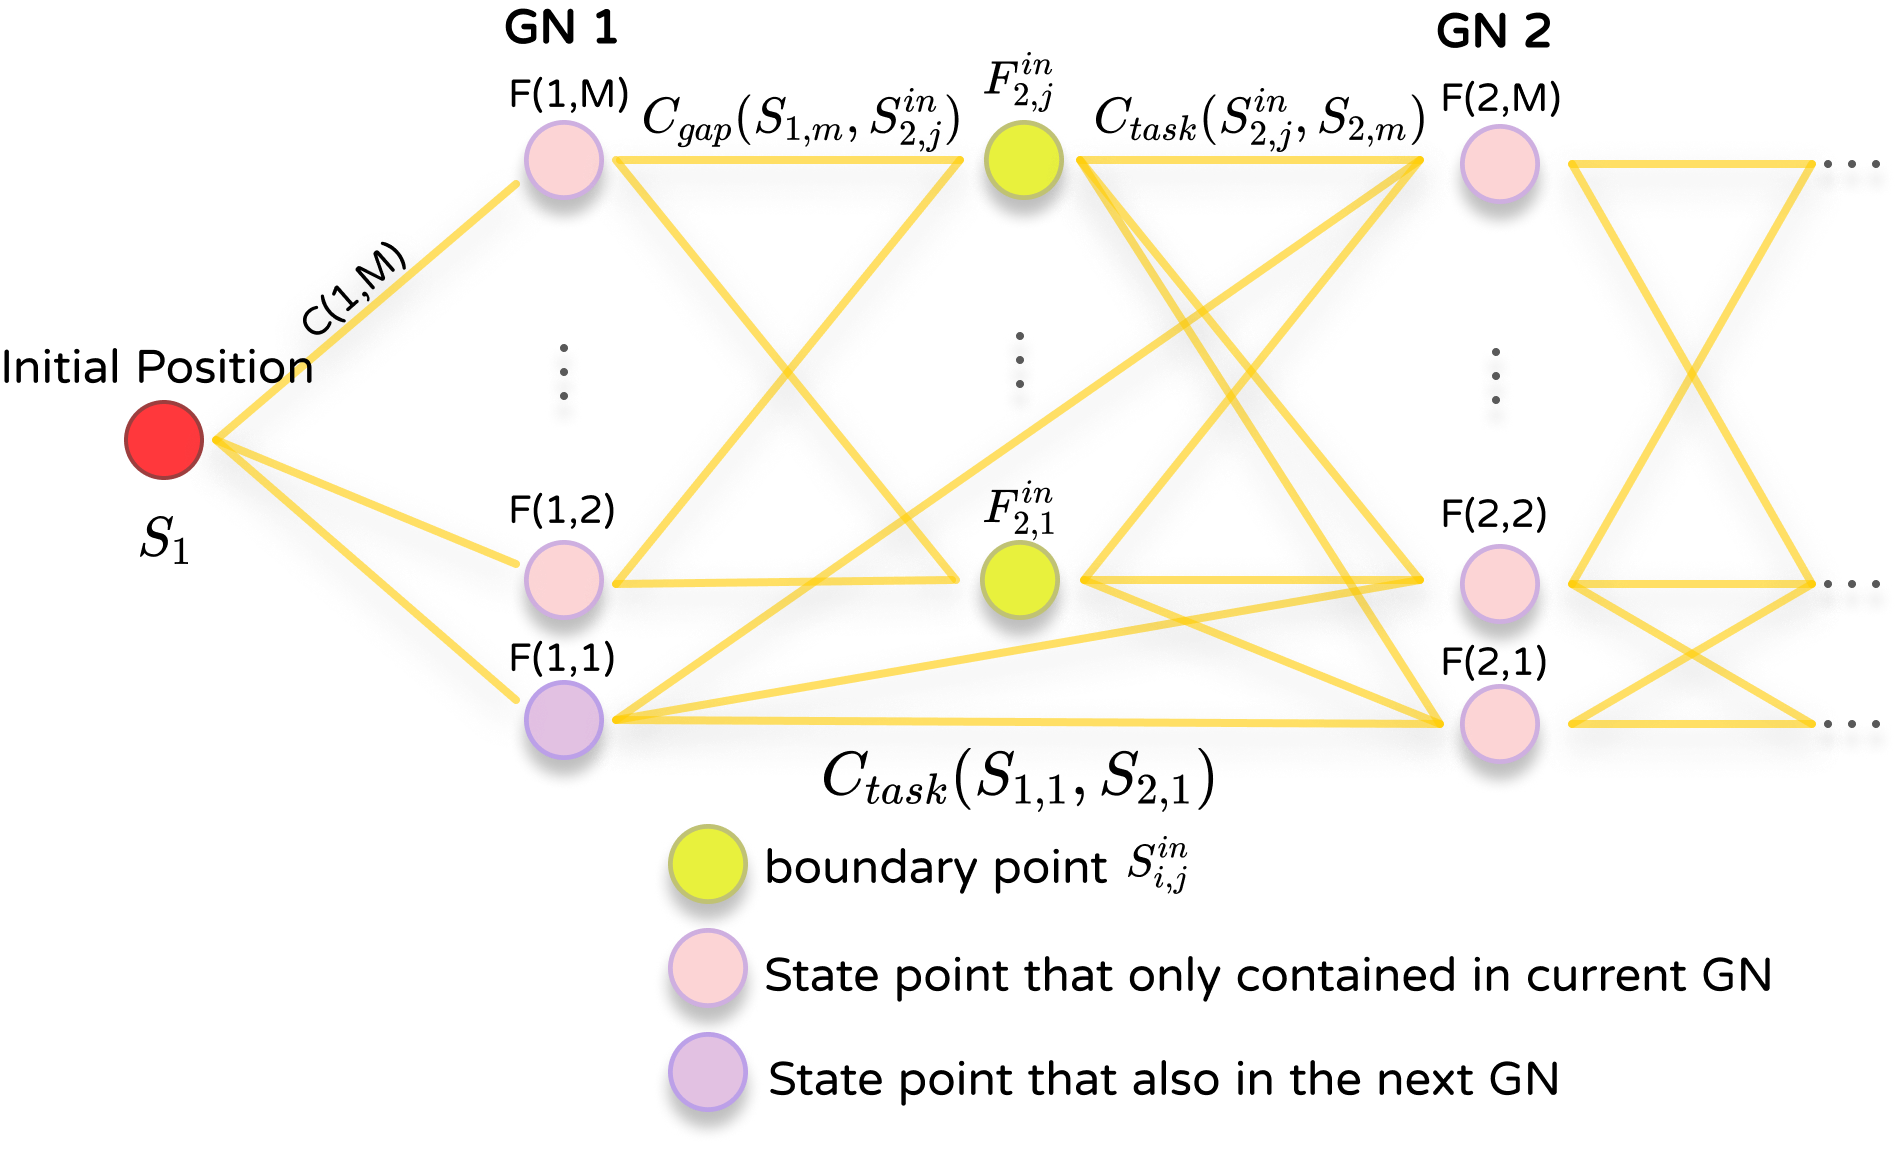
\includegraphics[width = 1 \linewidth]{figures/global-algorithm-flowchart.png}
    \caption{ Stage-wise state-transition structure of the proposed ORE dynamic programming algorithm. The mission is decomposed into per-GN stages: within the communication region of each $GN_i$, discrete exit-state points (pink: contained only in the current GN; purple: already inside the next GN's coverage) and boundary entry state points $S^{in}_{i,j}$ (green) are enumerated. Each inter-stage transition cost is decomposed into a gap-segment cost $C_{gap}$ and a task-segment cost $C_{task}$. Starting from the initial state $S_1$, the algorithm recursively accumulates the minimum reached energy $F_{i,m}$ over all feasible predecessor states, turning the continuous JHVSO problem into a shortest-path search.}
   \label{fig:rough_process}
\end{figure}

In this section, we present the algorithmic framework designed to address the joint speed optimize problem.
Specifically, we delineate the calculation of the local transition cost between consecutive state points, formulate the recursive solution for the Optimal Reached Energy (ORE) sub-problem, and establish the theoretical optimality of the global scheduling algorithm.
The candidate state sets $GN_i$ are pre-filtered by the altitude bounds $h_{\min}\le h\le h_{\max}$ during state-space construction, so the dynamic program operates on altitude-feasible states only.

\subsection{Calculation for Local Transition Cost}

Fig.~(\ref{fig:rough_process}) described how algorithm calculating through ground nodes.
The proposed algorithm operates stage-by-stage across consecutive ground nodes.
Initiating from the initial state $S_0$, the algorithm evaluates the ORE sub-problem for $GN_1$ to determine $F_{1,m}$ for all candidate states $m \in GN_1$.
This is achieved by compounding the initial condition with the transition cost from $S_0$ to each state point associated with $GN_1$.
Once the optimal values for the first stage are derived, they serve as the foundational prefix costs for the subsequent stage.
By recursively integrating these state costs with the localized transition costs between $GN_1$ and $GN_2$, the search space is advanced sequentially.
Given its pivotal role as the building block of the recursive formulation, the accurate calculation of the local transition cost is paramount.

\begin{figure}[]
  \centering
   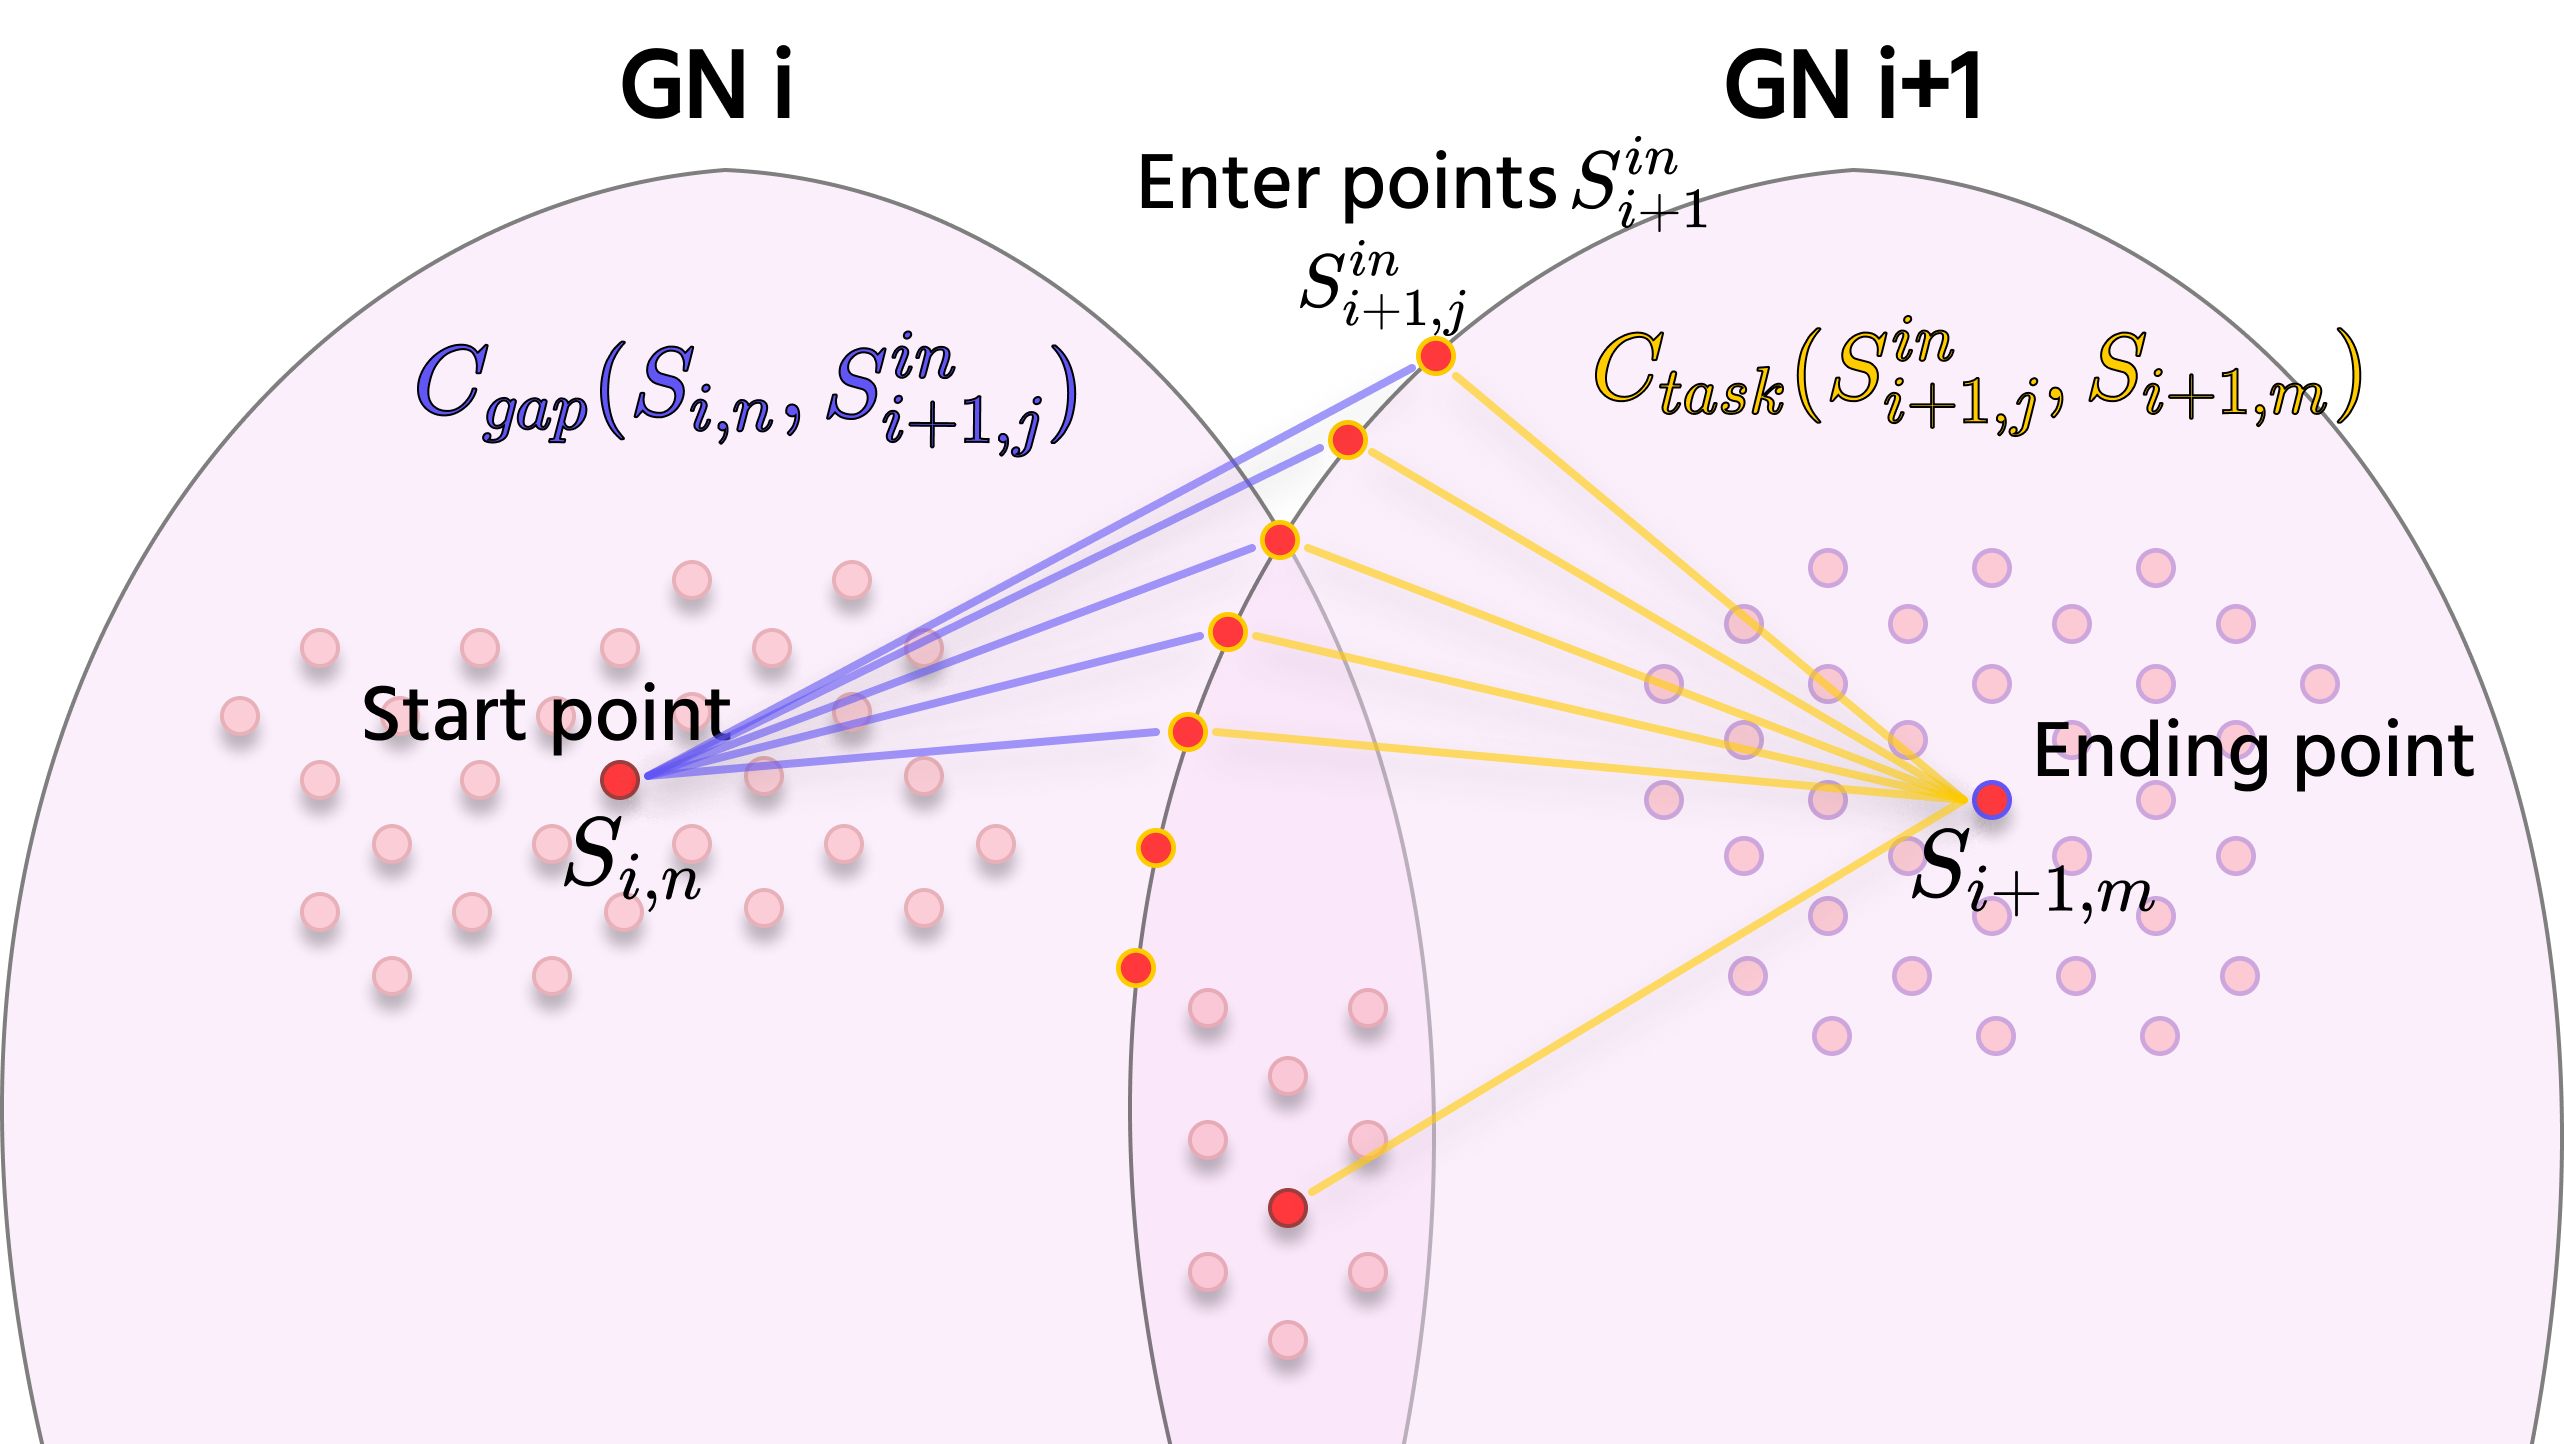
\includegraphics[width = 1\linewidth]{figures/transition-cost-case-1.png}
    \caption{Local transition cost between two state points $S_{i,n}$ (an exit state of $GN_i$) and $S_{i+1,m}$ (a target exit state in $GN_{i+1}$). When $S_{i,n}$ lies outside the coverage of $GN_{i+1}$, the transition is split at a boundary entry point $S^{in}_{i+1,j}$: a gap segment with cost $C_{gap}(S_{i,n}, S^{in}_{i+1,j})$, flown at the pitch-angle-dependent energy-optimal speed (Theorem~\ref{thm:optimal-range-speed}), followed by a task segment with cost $C_{task}(S^{in}_{i+1,j}, S_{i+1,m})$, flown at constant velocity that exactly fulfills the required collection duration $\tau_{i+1}$ (Theorem~\ref{thm:constant-speed}). The transition cost is the minimum compounded cost over all candidate entry points (Eq.~(\ref{equ:local_transition})).}
   \label{fig:transition-cost-case-1}
\end{figure}

Fig.~(\ref{fig:transition-cost-case-1}) show the way to evaluate the transition cost between exit state $S_{i,n}$ at stage $i$ and a target state  $S_{i+1,m}$ at stage $i+1$, the algorithm first evaluates their spatial alignment.
If the exit state already lies within the transmission coverage of the subsequent node $(S_{i,n} \in GN_{i+1})$, no gap cruising is required.
In this case, the transition cost is directly modelled as a straight-line flight spanning the distance $||S_{i,n},S_{i+1,m}||$ executed at a constant speed $v = ||S_{i,n},S_{i+1,m}||/\tau_{i+1}$, where $\tau_{i+1}$ represents the minimum required time for data collection duration.

Meanwhile, when the starting state resides outside the coverage of the next node $(S_{i,n} \notin GN_{i+1})$, the flight path between $S_{i,n}$ and $S_{Pi+1,m}$, must be partitioned into a gap segment and a task segment.
The configuration of the candidate trajectories is dictated by the entry states $S^{in}_{i+1,j}$ of $GN^{in}_{i+1}$ in \textit{Definition. \ref{def:state}}.
The algorithm evaluates all candidate transitions by linking the exit state $S_{i,n}$ to each entry point $S^{in}_{i+1,j}$ to compute the gap transition cost $C_{gap}(S_{i,n},S^{in}_{i+1,j})$.
To optimize this unconstrained cruise phase, the look-up function $LUT(\gamma)$ defined in Eq.~(\ref{equ:lut}) is utilized, which pre-computes the energy-per-meter optimum from the horizontal and vertical propulsion models across pitch angles, subject to the component-wise speed limits.

Following the gap segment, the task transition cost $C_{task}(S^{in}_{i+1,j},S_{i+1,m})$ is computed for the data collection phase within the communication range.
The total local transition cost between the two states is then determined by identifying the optimal boundary entry point that minimizes the compounded energy of both segments:

\[C(S_{i,n},S_{i+1,m}) = \min_{\forall S^{in}_{i+1,j}\in GN^{in}_{i+1}}(C_{gap}(S_{i,n},S^{in}_{i+1,j})\]
\[+C_{task}(S^{in}_{i+1,j},S_{i+1,m}))\]


\begin{algorithm}
    \caption{local transition cost calculation between two states}\label{alg:local_transition_cost}  
    \begin{algorithmic}[1]
        \Require $S_{i,n},S_{i+1,m},S^{in}_{i+1},\tau_{i+1}$
        \If{$S_{i,n}\in GN_{i+1}$}
            \State $C(S_{i,n},S_{i+1,m})=p \left(\frac{||S_{i,n},S_{i+1,m}||}{\tau_{i+1}}\right)\times \tau_{i+1}$
        \Else
            \State //$\gamma(S_{i,n},S^{in}_{i+1,j})$ means the angle of pitch between two states
            \For{$\forall S^{in}_{i+1,j} \in GN^{in}_{i+1}$}
                \State $C_{gap}(S_{i,n},S^{in}_{i+1,j}) = LUT(\gamma(S_{i,n},S^{in}_{i+1,j}))\times ||S_{i,n},S^{in}_{i+1,j}||$
                \State $C_{task}(S_{i,n},S^{in}_{i+1,j}) = P \left(\frac{||S^{in}_{i+1,j},ƒS_{i+1,m}||}{\tau_{i+1}}\right)\times \tau_{i+1}$
                \State $C_{S^{in}_{i+1,j}} = C_{gap}(S_{i,n},S^{in}_{i+1,j})+ C_{task}(S_{i,n},S^{in}_{i+1,j})$
            \EndFor
            \State $$C(S_{i,n},S_{i+1,m}) = \min_{\forall S^{in}_{i+1,j}\in GN^{in}_{i+1}}(E_{S^{in}_{i+1,j}})$$
        \EndIf
    \end{algorithmic}
\end{algorithm}

\begin{lemma}
    For any given pair of state points $S_{i,n}$ and $S_{i+1,m}$ at consecutive stages $i$ and $i+1$, the local transition cost $C(S_{i,n}, S_{i+1,m})$ is the theoretical minimum energy path under the defined constraints.
\end{lemma}

\begin{proof}
    The transition cost calculation is bifurcated based on the spatial relationship between the exit state $S_{i,n}$ and the transmission range of the target ground node ($GN_{i+1}$).

    \begin{enumerate}[a)]
    \item In-Range Transition ($S_{i,n} \in GN_{i+1}$)

    When the exit state $S_{i,n}$ resides within the transmission coverage of the target ground node, the transition is categorized as pure task segment.
    The transition cost $C_{task}$ is computed based on the displacement (distance and altitude) between $S_{i,n}$ and $S_{i+1,m}$ over the required data collection duration $\tau_{i+1}$.
    As established in \textit{Theorem. \ref{thm:constant-speed}}, for any given horizontal distance and altitude differential, maintaining a constant velocity over mission required duration $\tau$ is the most energy-efficient flight strategy.
    Thus, the transition cost in this scenario is theoretical optimal.
    \item Out-of-Range Transition ($S_{i,n} \notin GN_{i+1}$)

    For scenarios where the starting state lies outside the target transmission range, the trajectory is partitioned into a "gap segment" and a "task segment" via the boundary entry points $S_{i+1,j}^{in} \in GN^{in}_{i+1}$.
    The validity of this decomposition relies on two fundamental properties:
        \begin{itemize}
        \item Non-aftereffect Property: The UAV’s flight energy consumption model is solely a function of instantaneous velocity, implying that propulsion energy is independent of the UAV's velocity history.
        Furthermore, the time constraint $\tau_{i+1}$ is strictly imposed on the task segment, leaving the gap segment unconstrained in time.
        Consequently, the transition process satisfies the non-aftereffect property, allowing the optimization of the two segments to be decoupled.
        \item Optimality: The optimality of the task segment is guaranteed by \textit{Theorem. \ref{thm:constant-speed}}.
        For the gap segment, \textit{Theorem. \ref{thm:optimal-range-speed}} demonstrates that the energy-optimal strategy is to maintain a constant speed that minimizes energy consumption per unit distance.
        \end{itemize}  
    By systematically evaluating all feasible entry points on the transmission boundary and integrating the independently optimized costs for the gap and task segments, the resulting transition cost $C(S_{i,n}, S_{i+1,m})$ represents the theoretical optimum for the stage transition.
    \qed
    \end{enumerate}  
\end{proof}

\subsection{Solution for ORE and JHVSO Problem}

Before presenting the recursive solution, we first address a computational bottleneck inherent in the direct application of \textit{Algorithm. \ref{alg:local_transition_cost}}.
Suppose the preceding node $GN_i$ and current node $GN_{i+1}$ are discretized into $m$ and $n$ candidate states, respectively, and the transmission boundary of $GN_{i+1}$ is sampled by $j$ entry points.
Evaluating the ORE recurrence Eq.~(\ref{equ:ore_1}) by computing the local transition cost $C(S_{i,n},S_{i+1,m})$ independently for every state pair requires, for each of the $m\times n$  pairs, an enumeration of all $j$  entry points to identify the optimal compounded energy of the Gap and Task segments, resulting in a per-stage complexity of $O(m\times j \times n)$.

This overhead can be eliminated through a decoupled evaluation order.
Observe that in the compounded transition cost of Eq.~(\ref{equ:ore_1}), the Gap-segment term $C_{gap}(S_{i,n},S^{in}_{i+1,j})$ is independent of the target state $S_{i+1,m}$, the Task-segment term $C_{task}(S^{in}_{i+1,j},S_{i+1,m})$ is independent of the exit state $S_{i,n}$, and the prefix energy $F_{i,n}$ is independent of the entry point.
Substituting Eq.~(\ref{equ:local_transition}) into the ORE recurrence and rearranging the two minimizations therefore yields
\begin{align}\label{equ}
    &F_{i+1,m} = \min_{\forall S^{in}_{i+1,j}}(\min_{\forall S_{i,n} \notin GN_{i+1}}(F_{i,n} + C_{gap}(S_{i,n},S^{in}_{i+1,j}) + 
    \nonumber
    \\ &C_{task}(S^{in}_{i+1,j},S_{i+1,m})))
\end{align}

The inner minimization is precisely the ORE value of the entry state (Definition. \ref{def:ORE}),

\begin{equation}
F^{in}_{i+1,j} = \min_{\substack{S_{i,n} \in GN_i \\ S_{i,n} \notin GN_{i+1}}} \big\{ F_{i,n} + C_{gap}(S_{i,n}, S^{in}_{i+1,j}) \big\},
\label{equ:fin}
\end{equation}
i.e., the minimum energy of completing the first $i$ tasks and cruising to the boundary point $S^{in}_{i+1,j}$.
It depends only on the exit states and the entry points, and is therefore computed exactly once for each exit-state--entry-point pair and reused by all $n$ target states.
The outer minimization then projects the entry costs onto the exit states through the task segments,
\[
F_{i+1,m} = \min\Big\{ \underbrace{\min_{j} \big\{ F^{in}_{i+1,j}+ C_{task}(S^{in}_{i+1,j}, S_{i+1,m}) \big\}}_{\text{via boundary entry}},\;
\]
\[
 \underbrace{\min_{S_{i,n} \in GN_i , S_{i,n} \in GN_{i+1}} \big\{ F_{i,n} + C_{task}(S_{i,n}, S_{i+1,m}) \big\}}_{\text{overlap, direct task}} \Big\}
\]
The evaluation is thus reorganized into two decoupled phases with complexities $O(m \times j)$ and $O(j \times n)$, reducing the per-stage overhead from $O(m \times j \times n)$ to $O(m \times j + j\times n)$.
Transitions originating from overlapping states that already reside within the coverage of $GN_{i+1}$ involve no entry points and are evaluated directly through the Task segment, which is unaffected by this restructuring.
Crucially, the rearrangement is an exact algebraic restructuring rather than an approximation: every candidate trajectory composed of an exit state, an entry point, and a target state is still examined, and each is examined exactly once, so the resulting ORE values are identical to those of the pairwise evaluation.
The validity of compounding the prefix energy with the Gap cost at a boundary entry point—without regard to the target state that follows—is precisely the non-aftereffect property established in \textit{Theorem. \ref{thm:aftereffect}}, applied here with the entry point acting as the intermediate state.
We now formalize this two-phase evaluation in the ORE algorithm.

With the local transition cost formalized, we extend the framework to solve the Optimal Reached Energy (ORE) sub-problem recursively.
The ORE sub-problem at stage $i+1$, denoted as $F_{i+1,m}$, aims to find the energy-minimal trajectory that completes data collection for the first $i+1$ ground nodes, terminating precisely at the state $S_{i+1,m}$.
This framework systematically leverages the optimized state values $F_{i,n}$, computed from the preceding stage $i$.

\begin{figure}[]
  \centering
   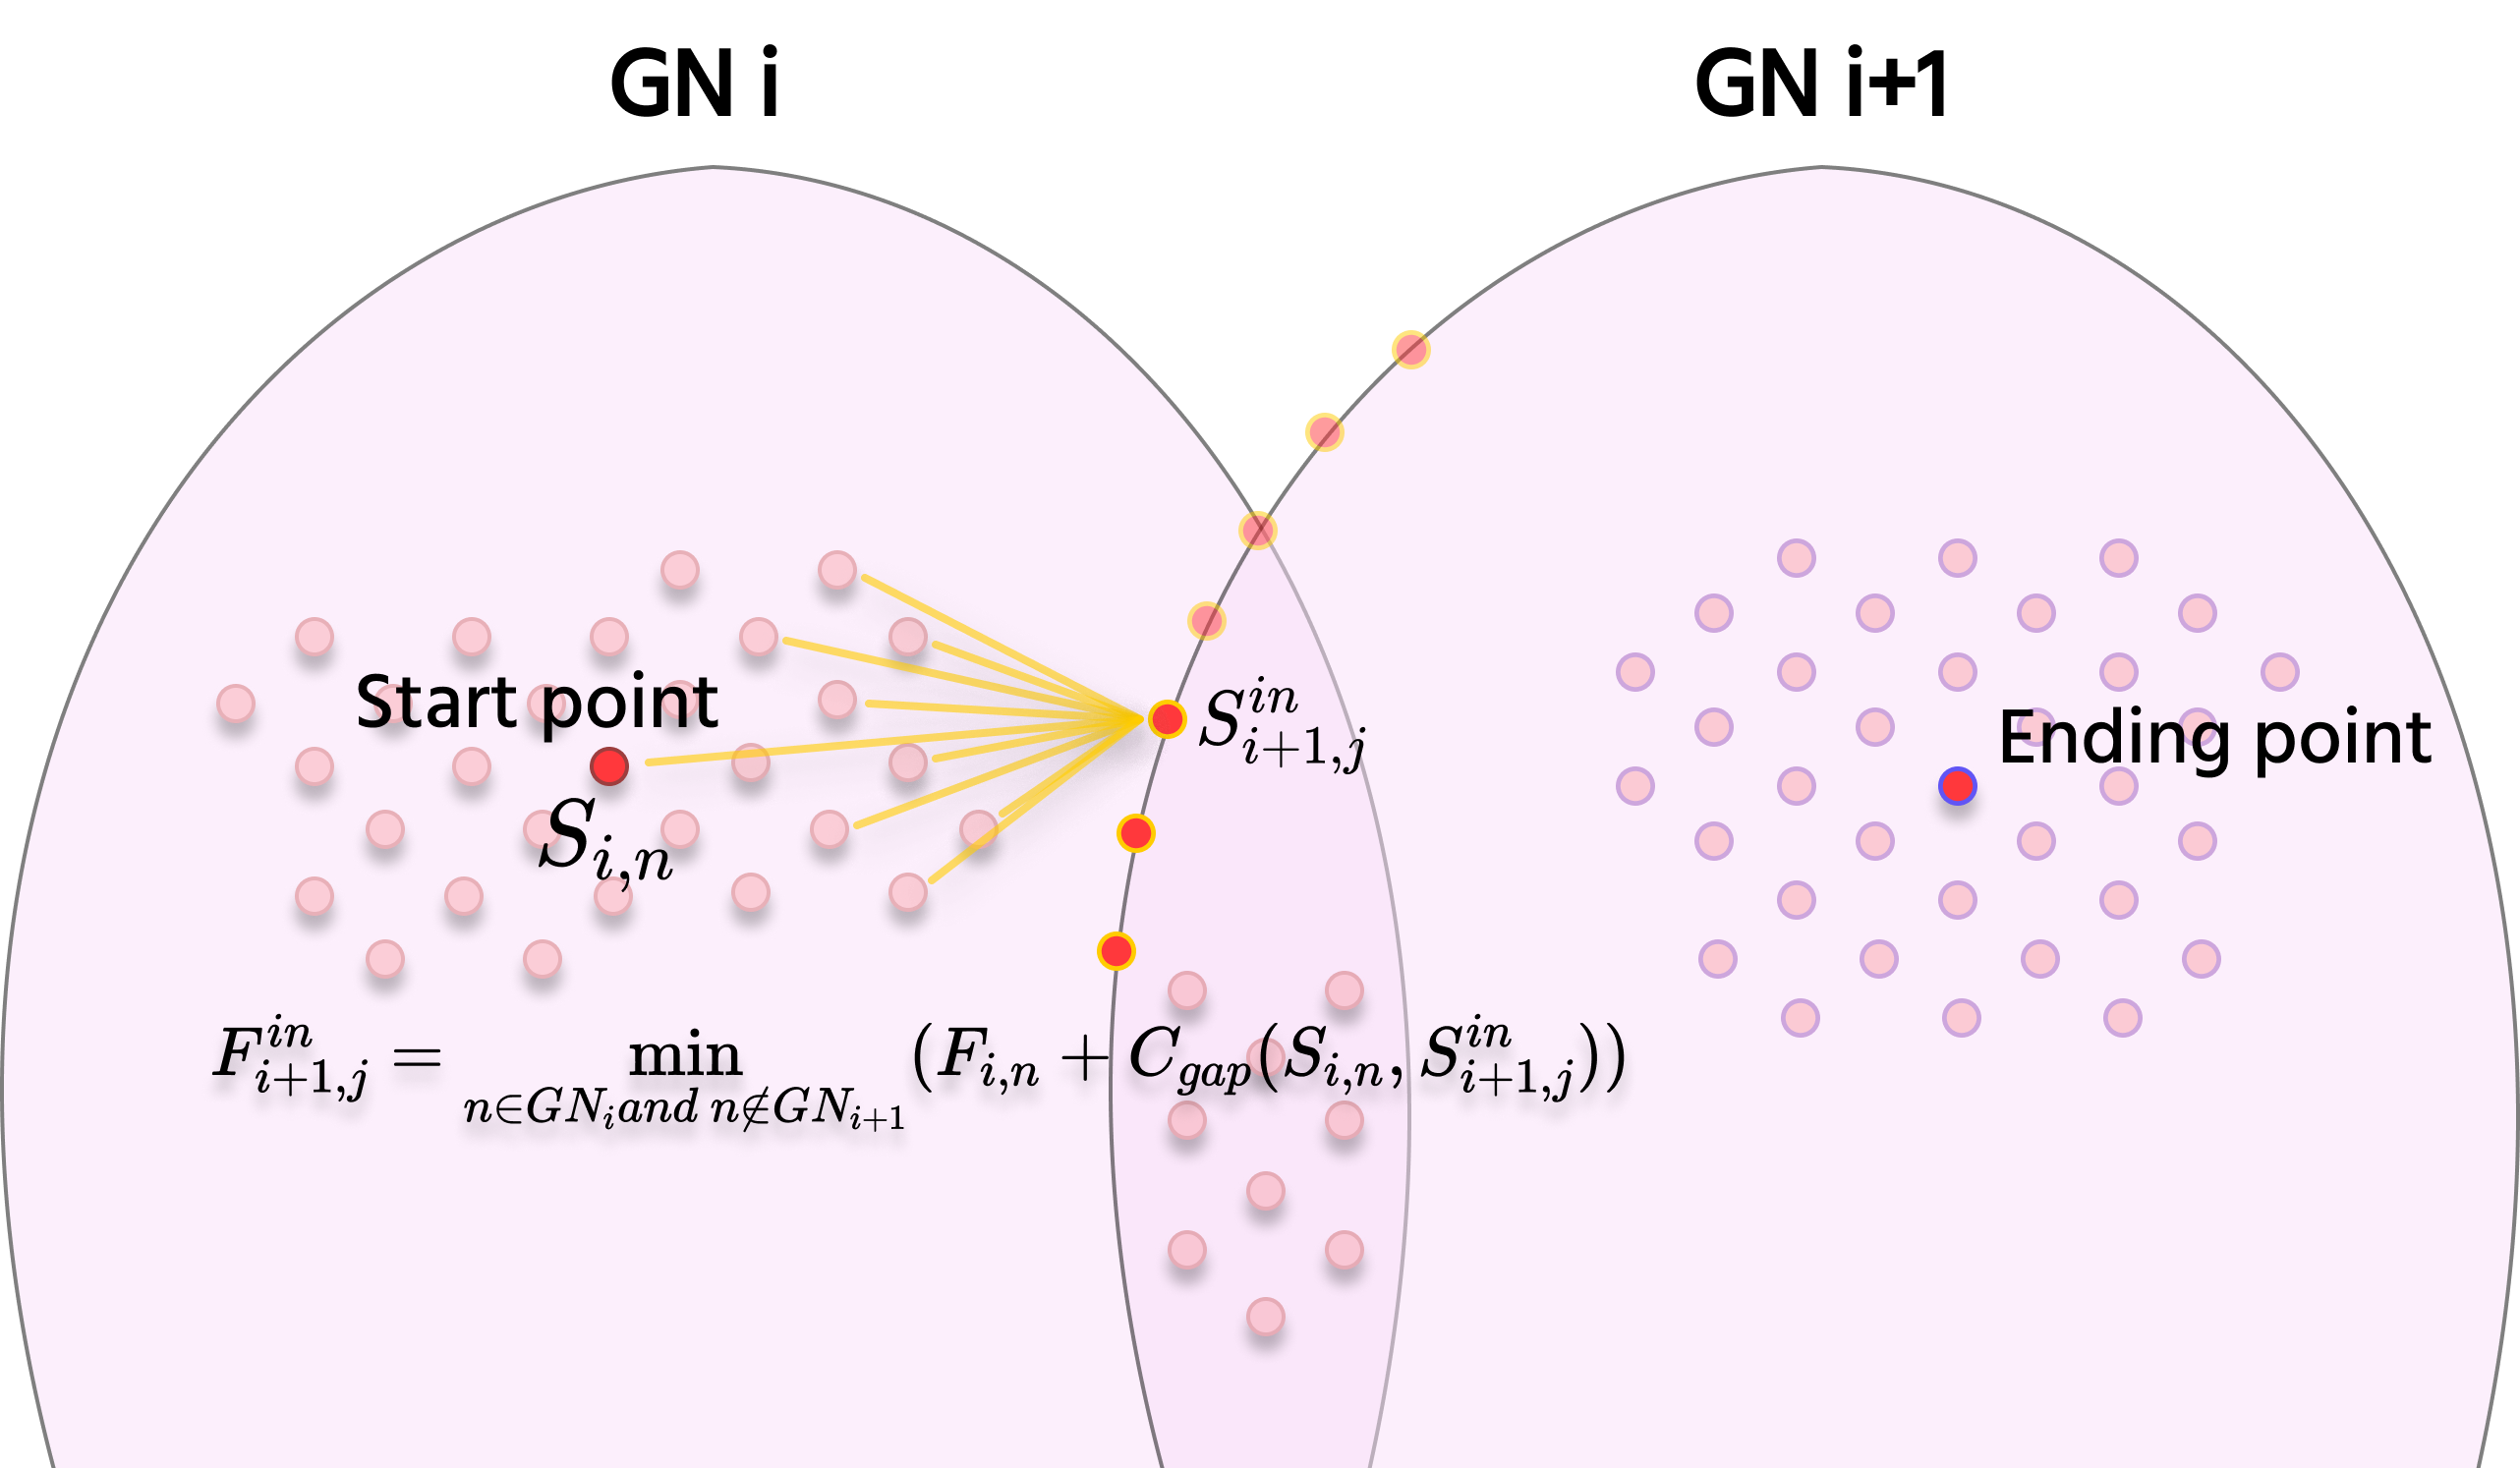
\includegraphics[width = 1\linewidth]{figures/transition-cost-case-2.png}
    \caption{ The energy cost of the mid-stage state point $F^{in}_{i+1}$ is computed by considering all state points from the previous stage that outside the communication range of $GN_{i+1}$.
    For each feasible predecessor state, the accumulated energy cost is added to the gap cost from that state to $S^{in}_{i+1}$.
    The minimum of these total costs is then taken as the energy cost of $F^{in}_{i+1}$}\label{fig:to_mid_stage}
\end{figure}

The calculation filters all candidate states from the previous stage that do not overlap with the current node's range, satisfying $S_{i,n}\notin GN_{i+1}$.
By mapping the gap costs  $C_{gap}$ from these disjoint states to the boundary entry points, the intermediate cost $F^{in}_{i+1,j}$ is minimized over the sum of the accumulated prefix energy and the cruise energy.

Once the optimal intermediate energy $F^{in}_{i+1,j}$ to reach the entry boundaries is established, the task costs $C_{task}(S^{in}_{i+1,j},$ $S_{i+1,m})$ are incorporated to project the path to the final state $S_{i+1,m}$, yielding a candidate value $\alpha$.
Simultaneously, the algorithm accounts for overlapping cases where prior states already reside within the transmission range of the current node $(S_{i,n} \in GN_{i} \cap GN_{i+1})$.
For these overlapping states, the task cost $C_{task}(S_{i,n},S_{i+1,m})$ is computed directly without a gap phase, yielding a candidate value $\beta$.
The ultimate ORE value $F_{i+1,m}$ is then determined by selecting the absolute minimum between these two operational pathways.


\begin{algorithm}
    \caption{ORE}\label{alg:ORE}  
    \begin{algorithmic}[1]
        \Require $GN_i, GN_{i+1},F_i,S^{in}_{i+1},\tau_{i+1}$
        \For{$S^{in}_{i+1,j} \in S^{in}_{i+1}$}
            \For{$\forall S_{i,n}\in GN_{i}\  and\  S_{i,n}\notin GN_{i+1}$}
                \State $F^{in}_{i+1,j} = \min(F_{i,n}+C_{gap}(S_{i,n},S^{in}_{i+1,j}))$
            \EndFor
        \EndFor
        \For{$S^{in}_{i+1,j} \in S^{in}_{i+1}$}
            \State $\alpha = \min (F^{in}_{i+1,j} + C_{task}(S^{in}_{i+1,j},S_{i+1,m}))$
        \EndFor
        \For{$\forall S_{i,n}\in GN_{i}\  and\  S_{i,n}\in GN_{i+1}$}
            \State $\beta = \min (F_{i,n} + C_{task}(S_{i,n},S_{i+1,m}))$
        \EndFor
        \State $F_{i+1,m} = min(\alpha,\beta)$
    \end{algorithmic}
\end{algorithm}
Once the ORE values are resolved for all stages, the global Joint horizontal-vertical speed optimization (JHVSO) problem can be straightforwardly solved.
The global energy-optimal trajectory encompassing all N ground nodes is obtained by identifying the minimum cost among all feasible terminal states at the final stage, expressed as $\min(F_N)$.

\begin{algorithm}
    \caption{JHVSO}\label{alg:JHVSO}  
    \begin{algorithmic}[1]
        \Require $S_0,GN_{1 \dots N},\tau_{1\dots N},h_f$
        \For{$GN_i \in GN_{1 \dots N}$}
            \For{$S_{i,m} \in GN_{i}$}
                \State $F_{i,m} = ORE(F_{i-1},S_{i,m})$
            \EndFor
        \EndFor
        \State $JHVSO = \min_{h=h_f}(F_{N})$
    \end{algorithmic}
\end{algorithm}


\begin{figure}[]
  \centering
   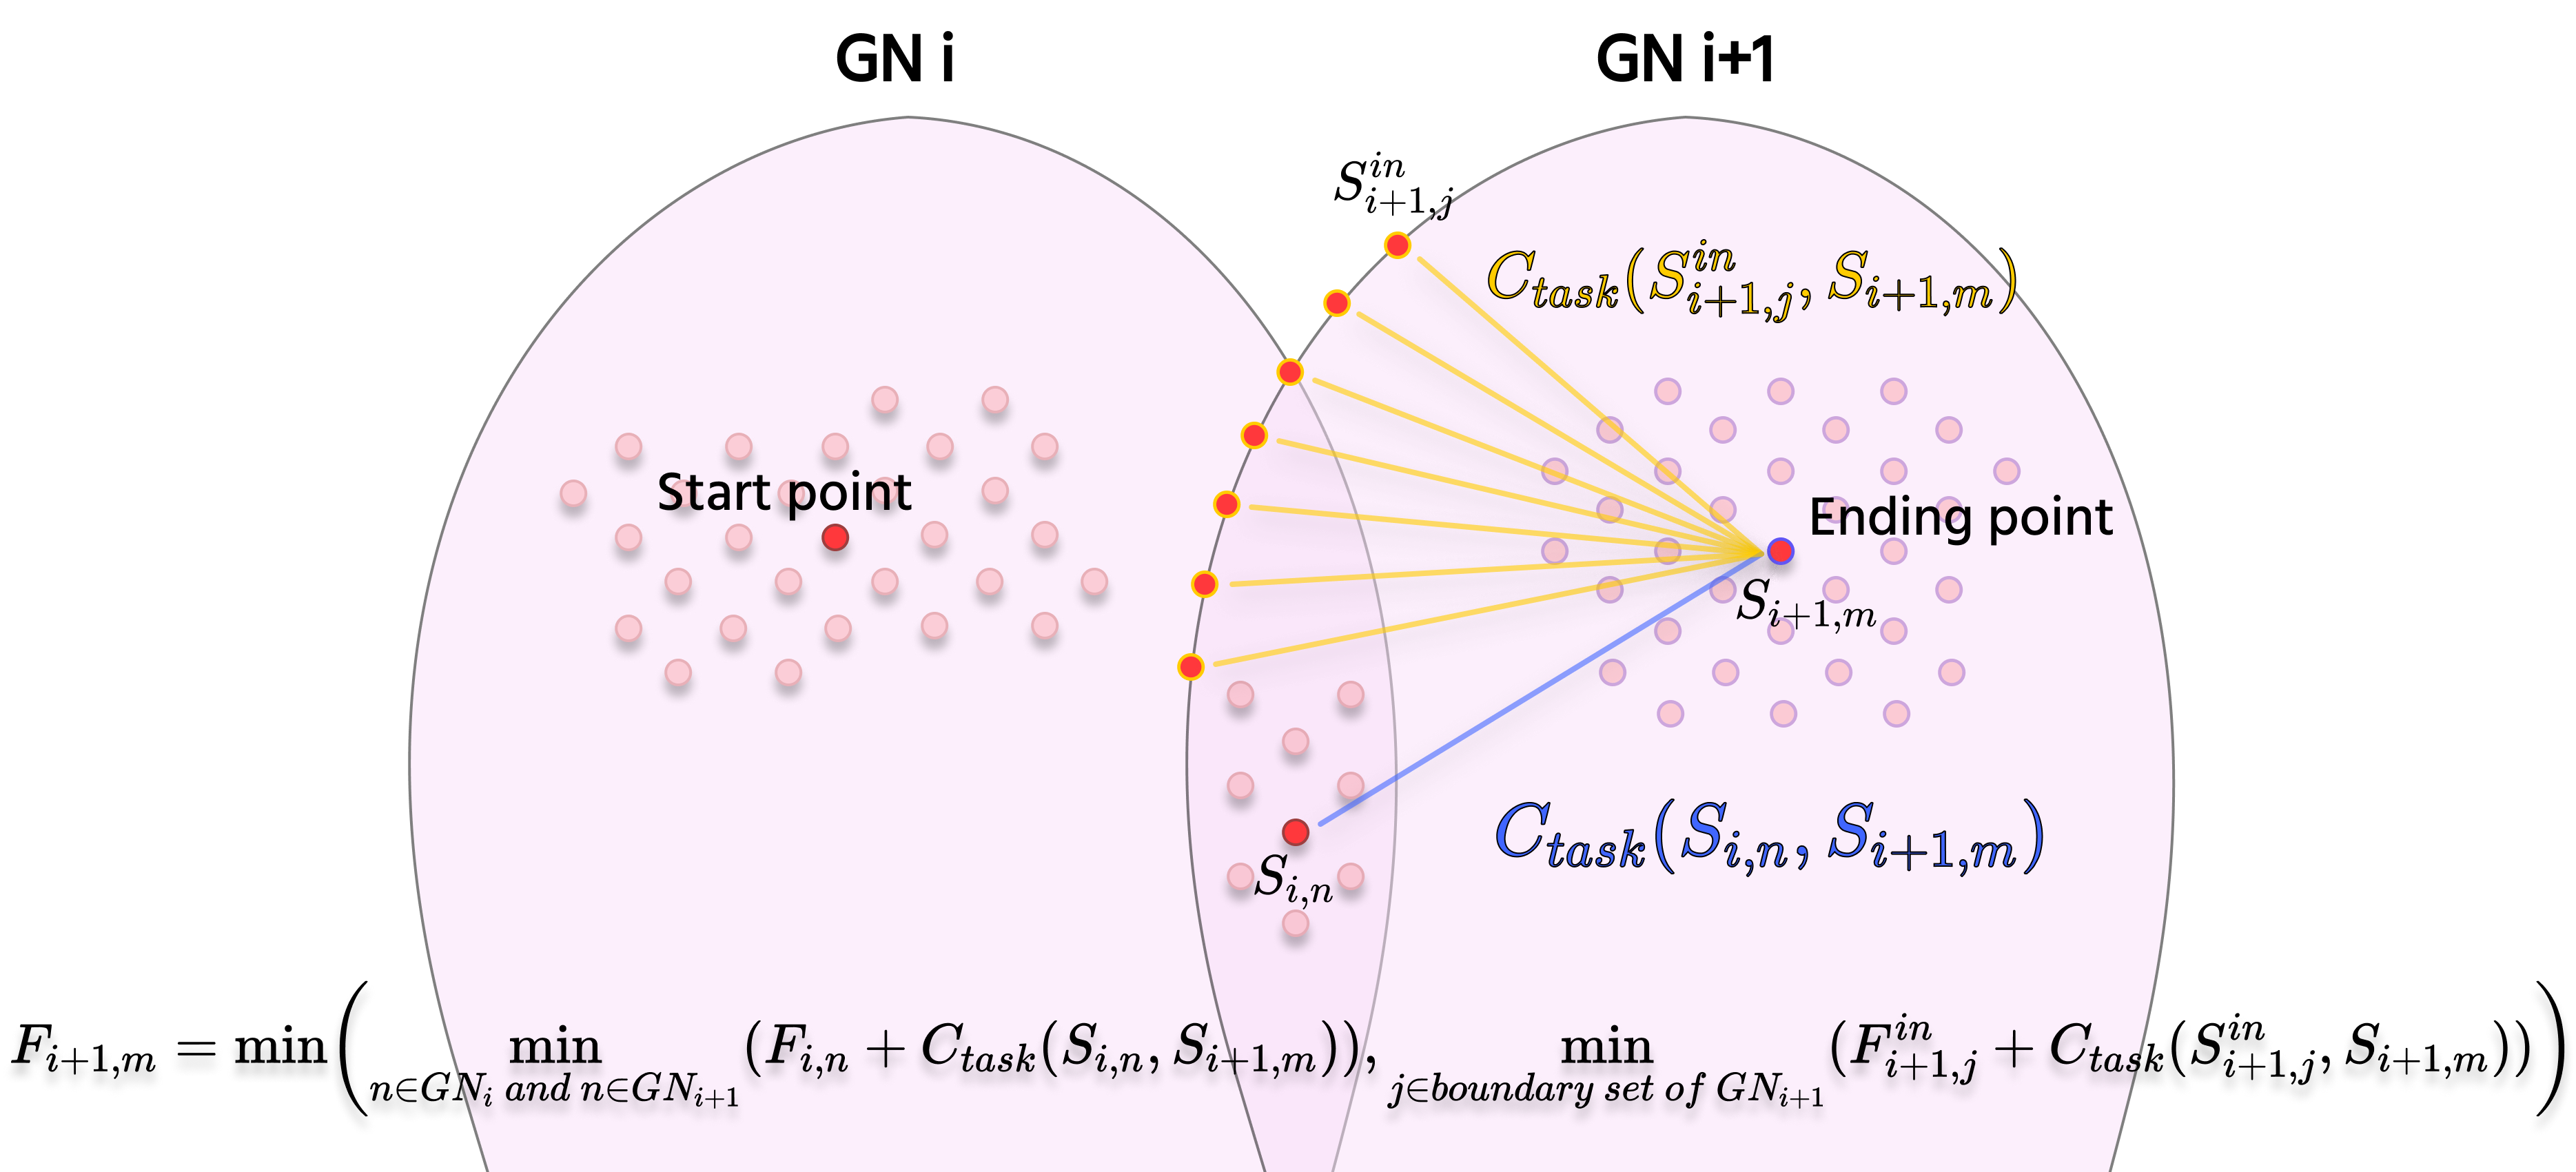
\includegraphics[width = 1\linewidth]{figures/transition-cost-case-3.png}
    \caption{The energy cost of $S_{i+1,m}$ is obtained by evaluation all state points from the previous stage that are within the communication range of the current ground node $S_{i,n} \in GN_i\&GN_{i+1}$ and the mid-stage state points $S^{in}_{i+1}$ .
    For each feasible predecessor state, the corresponding task cost is added to its accumulated energy cost.
    The minimum resulting cost is assigned as the energy cost of $S_{i+1,m}$}\label{fig:from_mid_stage}
\end{figure}

\begin{theorem}
    For any stage $i \in \{1, 2, \dots, N\}$ and any discrete state $S_{i,m} \in GN_{i}$, the cumulative minimum energy consumption $F_{i,m}$ calculated by the proposed ORE algorithm is exactly equal to the theoretical global minimum energy consumption $G(S_{i,m})$, which means:
    $$F(S_{i,m}) = G(S_{i,m}), \quad \forall S_{i,m} \in GN_i, i \in {1, 2, \dots, N}$$
\end{theorem}


\begin{proof}
    The cumulative minimum energy consumption $F_{i,m}$ for state $S_{i,m}$ is calculated by finding the trajectory with minimum energy consumption from all possible states of previous stage.

$$F_{i,m} = \min_{\forall S_{i-1,n} \in GN_{i-1}} \{F_{i-1,n} + C(S_{i-1,n},S_{i,m})\}$$

The transition cost from these possible states to the target states has no aftereffect, as we have proved in \textit{Theorem.\ref{thm:aftereffect}}.
So we can using the principle of mathematical induction on the stage index $i$.

The induction runs over the stage boundaries, i.e., the exit states.
Within each stage, the value of every entry state is obtained from the preceding exit states through Eq.~(\ref{equ:fin}), whose optimality follows from the same non-aftereffect argument applied with the entry point as the intermediate state (\textit{Theorem.\ref{thm:aftereffect}}); hence it suffices to establish $F(S_{i,m}) = G(S_{i,m})$ at the exit states.

\textit{Base Case ($i = 1$):} At the beginning of the mission, the UAV departs from the unique initial deployment position $S_0$.
To reach any target state $S_{1,m} \in GN_1$ at the end of the first stage, there is no historical trajectory or prior decision path.
Therefore, the theoretical global minimum energy $G(S_{1,m})$ consists uniquely of the single-step transition from $S_0$ to $S_{1,m}, \forall m\in GN_1 $, which can be expressed as $G(S_{1,m}) = C(S_0, S_{1,m})$.
Since the local transition cost has been proven to be optimal above, it follows that $F(S_{1,m}) = G(S_{1,m})$ holds strictly for all $S_{1,m} \in GN_1$.

\textit{Inductive Hypothesis:} Assume that the theorem holds true for stage $i-1$.
That is, for any discrete state $S_{i-1,n}$ within the state space $GN_{i-1}$, the algorithmic cumulative cost satisfies the following condition:

$$F(S_{i-1,n}) = G(S_{i-1,n}), \quad \forall S_{i-1,n} \in GN_{i-1}$$

\textit{Inductive Step:} We now evaluate the optimality of the algorithm at stage $i$ .
Consider an arbitrary state $S_{i,m} \in GN_i$.
Due to the spatial and temporal continuity of the flight trajectory, any globally optimal path reaching $S_{i,m}$ must pass through a specific boundary state at the preceding stage $GN_{i-1}$.
Therefore, the theoretical absolute minimum energy $G(S_i,n)$ can be mathematically expanded into a two-stage optimization form:

% \begin{align}\label{equ}
%     &G(S_{i,m}) =  \min_{\forall S_{i-1,n} \in GN_{i-1}}  \{G(S_{i-1,n}) +
%     \nonumber
%     \\ & \textit{Theoretical transition cost  from } S_{i-1,n} \textit{ to } S_{i,m} \}
%     \nonumber
% \end{align}

$$G(S_{i,m}) = \min_{\forall S_{i-1,n} \in GN_{i-1}} { \{G(S_{i-1,n}) + C^*( S_{i-1,n} , S_{i,m} )\}}$$

By invoking the non-aftereffect property established above, the transition cost from $S_{i-1,n}$ to $S_{i,m}$ is fully decoupled from the trajectory prior to stage $i-1$.
Furthermore, as demonstrated in Subsection 5.1, the local scheduling method guarantees that the calculated cost $C(S_{i-1,n}, S_{i,m})$ reaches the physical lower bound.
Consequently, the theoretical transition cost matches the algorithmic transition cost, which simplifies the equation to:


$$G(S_{i,m}) = \min_{\forall S_{i-1,n} \in GN_{i-1}} { \{G(S_{i-1,n}) +  C(S_{i-1,n} , S_{i,m})\} }$$


Next, we substitute the inductive hypothesis $G(S_{i-1,n}) = F(S_{i-1,n})$ into the optimization term, yielding:


$$G(S_{i,m}) = \min_{\forall S_{i-1,n} \in GN_{i-1}} { \{F(S_{i-1,n}) + C(S_{i-1,n}, S_{i,m})\} }$$


By the principle of mathematical induction, since the base case holds and the inductive step preserves this equality, the relation $F(S_{i,m}) = G(S_{i,m})$ is valid for all stages $i \in \{1, 2, \dots, N\}$.
This completes the proof.
\qed
\end{proof}

%%%%%%%%%%%%%%%%%%%%%%%%%%%%%%%%%%%%%%%%%%%%%%%%%%%%%%%%%%%%%%%%%%%%%%%%%%%%%%%%%%
%%%%%%%%%%%%%%%%%%%%%%%%%%%%%%%%%%%%%%%%%%%%%%%%%%%%%%%%%%%%%%%%%%%%%%%%%%%%%%%%%%
 

 \section{Simulation}
\label{sec:simulation}

To rigorously evaluate the performance of our proposed joint horizontal-vertical speed optimization algorithm, we consider a multi-rotor UAV deployed for distributed ground nodes data collection missions.

The power consumption of the UAV during horizontal flight is captured by a realistic, empirically validated non-linear function of its forward velocity $v$, expressed as $P_\parallel(v) = c_1 v^3 + c_2 v^2 + c_3 v + P_{mh}$.
Based on empirical flight test configurations from~\cite{Energy-Efficient-POI}, the non-linear coefficients are specified as $c_1 = 0.07$, $c_2 = 0.0391$, and $c_3 = -13.196$, with the baseline hovering power $P_{mh}$ being $390.95$ W .
For vertical flight, we use Eq.~(\ref{equ:v_1}) with $k_1 = 0.8554$, $k_2 = 1.9051$, $c_1 = 0.3177$, and $mg = 63.81\,\mathrm{N}$.
The parameters $k_1$ and $c_1$ are adopted from~\cite{PowerConsumptionModel}, while $k_2$ and $mg$ are calibrated to give a hovering power of approximately $390.8\,\mathrm{W}$, close to the horizontal model's $P_{mh}=390.95\,\mathrm{W}$.
The horizontal and vertical speeds of the UAV are restricted to $V_{\parallel}^{\max} = 20$ m/s and $V_{\perp}^{\max} = 10$ m/s, respectively, while its maximum-range speed-defined as the speed that maximizes aerodynamic efficiency-is determined to be $v_{\mathrm{best}} = 13.99$ m/s by minimizing $P_{\parallel}(v_{\parallel})/v_{\parallel}$.

In our simulation environment, a set of ground nodes (GNs) are deployed along a straight-line, and each $GN_i$ is assigned a random coordinate along the axis.
By default, the total number of GNs, denoted as $N_{GN}$, is set to 20, with spacing between consecutive GNs averaging 60 m.
To emulate realistic deployment heterogeneity, the parameters associated with each GN are not fixed to a single global value: as listed in \textit{Table. \ref{tbl:parameters}}, the parameter of each individual GN is independently and uniformly sampled within its per-GN variation range, so that different GNs within the same mission exhibit heterogeneous communication coverages and data requirements.
On this basis, each controlled experiment varies the default value of one parameter (or two coupled parameters, as in Fig.~(\ref{fig:sim})(f)) at a time, while all the remaining parameters follow the default configuration with the per-GN randomization preserved.

\begin{table}%[]
\caption{Default parameter setting.
The \emph{default value} is the mean used when a parameter is not being scanned; the \emph{per-GN variation range} is the uniform sampling interval for each individual GN.
In each controlled experiment, only the default value of the scanned parameter is varied, while all other parameters are sampled per GN from their variation ranges.}\label{tbl:parameters}
\begin{tabular*}{\tblwidth}{lcc}
\toprule
 Parameter & Default & Variation Range \\ % Table header row
\midrule
 Average\ $PL\ (dB)$ & 85  & [83 86]\\
 Average\ $D_i\ (Mbit)$ & 88 & [72 100]\\
 Nominal\ SINR\ $\Gamma_i$ & 15 & [12 18]\\
 Parameter\ $\mu _{LoS}\ (dB)$& 1.3 & [1 1.6]\\
 Parameter\ $\mu _{NLoS}\ (dB)$& 35 & -\\
 Average distance\ $(m)$& 60 & [30 80]\\
 Altitude\ bounds\ $[h_{\min},h_{\max}]$ (m) & [50, 150] & -\\
 Parameter\ $a$& 45 & [42 47]\\
 Parameter\ $b$& 0.25 & [0.2 0.3]\\
 Average\ number\ of\ $GN$& 20 & -\\
\bottomrule
\end{tabular*}
\end{table}


The air-to-ground wireless links between the flying UAV and the GNs are characterized by the communication model to account for typical urban blocking and shadowing effects.
The probability of establishing an LoS link depends heavily on the elevation angle $\theta$ between the UAV and the target GN, which is mathematically given by Eq.~(\ref{equ:PL}), where the environment-specific parameters are selected as $a = 45$ and $b = 0.25$.
The wireless communication operates at a standard carrier frequency of $f = 2.4 GHz$, with the speed of light defined as $c = 3 \times 10^8$ m/s.
The average excessive path losses for LoS and Non-Line-of-Sight (NLoS) connections are configured as $\mu_{LoS} = 1.3$ dB and $\mu_{NLoS} = 35$ dB, respectively.
A communication link is deemed valid and available for data upload if and only if the total path loss remains below a maximum allowable threshold of $PL = 85$ dB, which defines the continuous geometric coverage boundary shape for each GN.
The data upload adopts a channel bandwidth of $B = 1$ MHz and a per-GN nominal SINR $\Gamma_i$ sampled from $[12, 18]$ (default $15$), which yields a constant achievable rate $\bar{R}_i = B\log_2(1+\Gamma_i)$, about $4$ Mbps at the default. The required collection duration is then $\tau_i = D_i/\bar{R}_i$, which is approximately $22$ s on average under the default data volume $D_i = 88$ Mbit.

Each experimental configuration is repeated over $K = 5$ independent trials.
In every trial, the GN positions and the per-GN parameters are re-sampled uniformly from the variation ranges listed in \textit{Table.\ref{tbl:parameters}}, and the reported energy is the average over the $K$ trials.
The starting altitude is an exogenous mission constraint: the UAV departs and terminates at an altitude of $50$ m in the simulations of Sections~6.1--6.2, and at $100$ m in the real-world case study of Section~6.4.
The flight altitude is confined to $[h_{\min}, h_{\max}]=[50,150]$ m. The lower bound $50$ m matches the take-off/landing altitude, while the upper bound $150$ m is a representative operating ceiling for infrastructure-inspection missions: regulations permit altitudes above the $120$-m open-category limit when the UAV stays in close proximity to a structure (e.g., 14 CFR \S 107.51 allows flying up to 400 ft above a structure's top when within 400 ft of it~\cite{FAA-Part-107}).

% \begin{figure*}%[]
%   \centering
%    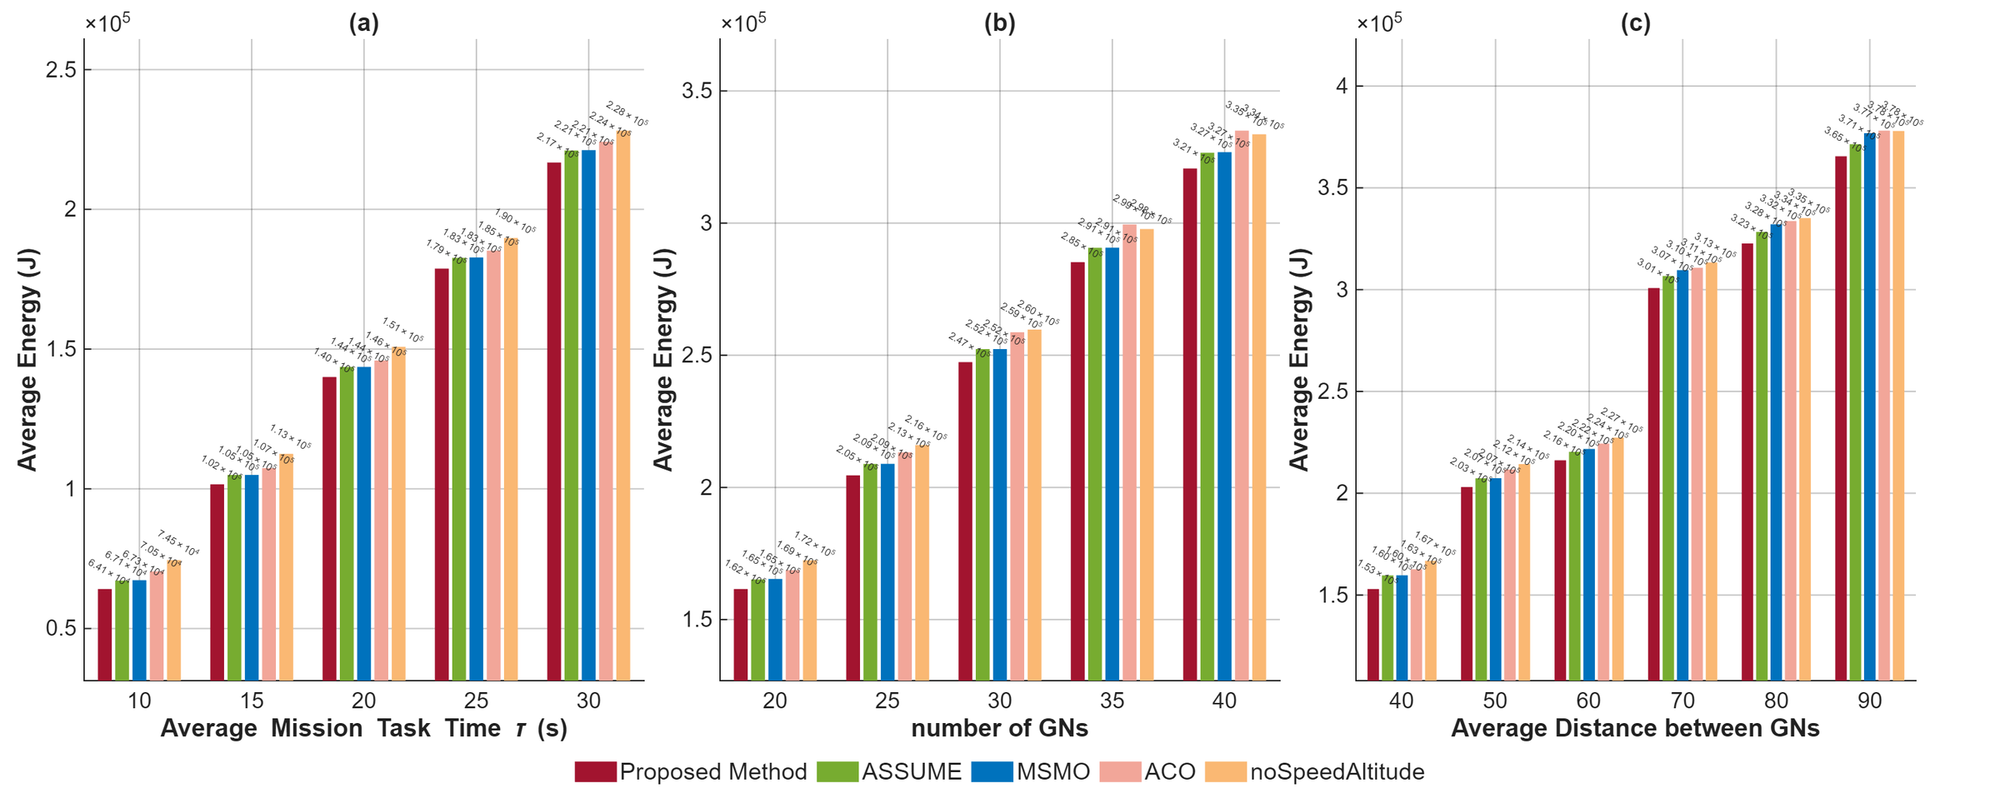
\includegraphics[width = 1\linewidth]{figures/simulation-comparison-alternative.png}
%     \caption{ }\label{fig1}
% \end{figure*}
\subsection{Baseline Algorithms}
We compare our proposed method with following base-line algorithms
\begin{itemize}
    \item \textit{ASSUME~\cite{assume}}: The ASSUME algorithm tackles the joint altitude and speed scheduling problem by discretizing the allowable 3D flight space.
    It quantizes the UAV's flight altitude into a finite set of horizontal segments.
    Within each fixed-altitude layer, it employs the Looking-Before-Crossing (LbC) technique to trace a shortest-path speed schedule across virtual spatial-temporal constraints.
    A dynamic programming (DP) framework is then superimposed to compute the optimal path across these different altitude levels.
    While ASSUME achieves mathematical optimality within its discrete framework, its performance is inherently bottlenecked by the resolution of its pre-defined altitude grid, often suffering from quantization errors that preclude finding the true continuous energy minimum.
    \item \textit{MSMO~\cite{msmo}}: This baseline introduces a speed scheduling that at any given iteration $t$, the UAV's horizontal velocity is dynamically evolved according to the rule: $v^{t}=v^{t-1}+R_{1}(v^{*}-v^{t-1})+R_{2}(1-A)(v_{max}-v_{min})$, where $R_{1}$ and $R_{2}$ are randomized tuning weights.
    The second term explicitly exploits the search space by pulling the speed toward the theoretical optimum $v^{*}$, whereas the third term injects random velocity perturbations to prevent the algorithm from stagnating in local energy minima.
    To handle the 3D environment, this iterative speed evolution is exhaustively repeated across all discrete altitude layers, ultimately outputting the altitude-speed pair that yields the lowest empirical energy cost.
    \item \textit{ACO~\cite{bi-aco}}: This approach decouples the scheduling dimensions, applying a deterministic rule for horizontal speed and a ACO based framework for vertical altitude.
    The horizontal transit speed over any target node $g_{i}$ is strictly dictated by the effective transmission range, calculated as $(f_{i}-\max(s_{i}, f_{i-1})) / \tau_{i}$.
    For the vertical dimension, an Ant Colony Optimization mechanism simulates pheromone deposition and heuristic path generation to navigate the discrete altitude levels.
    \item \textit{noSpeedAltitude}: Serving as a naive, worst-case benchmark, this algorithm entirely eliminates global dynamic optimization.
    Identical to the ACO method, the UAV's horizontal velocity is locked to a rudimentary calculation based on the effective transmission range and required time $\tau_{i}$.
    However, its altitude selection is reduced to a purely greedy mechanism: at each GN transition, the algorithm simply scans all feasible altitudes and forcibly selects the one that physically maximizes the geometric transmission coverage radius.
\end{itemize}
\begin{figure*}%[]
  \centering
   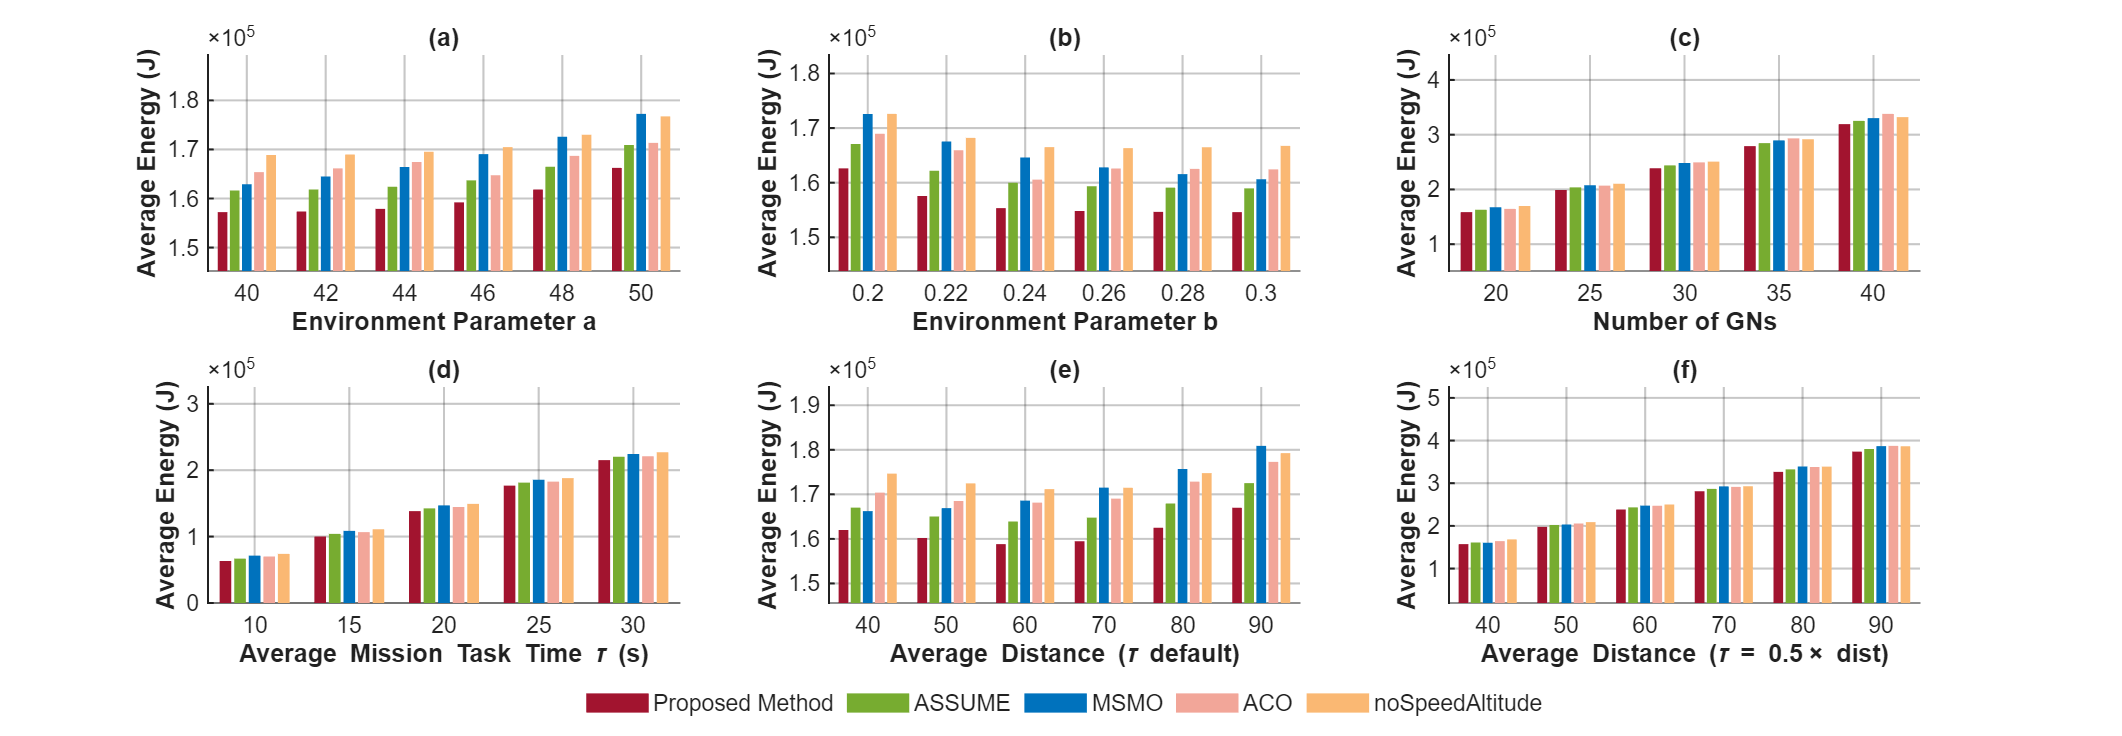
\includegraphics[width = 1.\linewidth]{figures/simulation-comparison.png}
    \caption{The UAV energy consumption of different algorithms.
    In (a), as the environment parameter $a$ --- equivalently, the elevation angle at which the LoS probability reaches $50\%$, given by $a+\ln(a)/b$ --- increases from 40 to 50 (from street canyons to extremely dense high-rise districts), the coverage region of each GN shrinks and the energy consumption of JHVSO, ASSUME, MSMO and noSpeedAltitude increases monotonically, with the increase steepening for $a\ge46$; the margin of JHVSO over MSMO widens from 3.6\% to 6.6\%.
    In (b), as the environment parameter $b$ increases, all methods first decrease in energy consumption and then stabilize once the LoS probability approaches its upper limit, with ACO and noSpeedAltitude showing minor non-monotonic wiggles.
    In (c), the energy consumption for each method increases constantly with more ground nodes added to the mission.
    In (d), all methods have the increase in energy consumption as the average time to complete data collection from one ground node increases.
    (e) and (f) show how the energy consumption of all methods changes as the distance between adjacent ground nodes increases.
    For (e), $\tau$ remains at its default value: the energy of JHVSO, ASSUME, ACO and noSpeedAltitude first decreases slightly (by about 2\%, with the minimum at an average distance of 60 m) and then increases, whereas MSMO rises monotonically, so that the margin of JHVSO over MSMO widens from 2.6\% at 40 m to 8.3\% at 90 m.
    For (f), $\tau$ grows proportionally with the distance, and the energy consumption of all methods increases monotonically.
    JHVSO achieves the lowest energy consumption in all 34 configurations, reducing energy by 1.7\%--5.8\% over the strongest baseline (ASSUME), 1.9\%--12.9\% over MSMO, 2.7\%--10.7\% over ACO, and 3.4\%--16.8\% over the greedy speed--height baseline (noSpeedAltitude).}\label{fig:sim}
\end{figure*}
\subsection{Simulation Results and Comparative Analysis}


Fig.~(\ref{fig:sim}) presents a comprehensive performance evaluation of the proposed \textit{JHVSO} algorithm alongside four baseline methods: ASSUME, MSMO, ACO, and noSpeedAltitude.

To thoroughly investigate the adaptability and robustness of these algorithms under diverse operational environments, we conduct six controlled experiments following the protocol of \textit{Table 1}: in each subfigure, the x-axis denotes the varied default value of the corresponding parameter, while the per-GN randomization within the variation ranges of \textit{Table 1} is preserved.
Each configuration is evaluated on three independent random instances, and the reported value is the average over the three instances.
To isolate the effect of the swept parameter from instance-to-instance fluctuations, the same random instances are reused across all sweep points of an experiment (common random numbers) so that only the swept parameter differs between neighboring points of a curve.

In Fig.~(\ref{fig:sim})(a), we evaluate the energy consumption as the environment parameter $a$ increases from 40 to 50.
Here the elevation angle $\theta=\arctan(h/d)$ measures how steeply the UAV looks down at a GN: $\theta=90^{\circ}$ corresponds to hovering directly overhead, while a small $\theta$ corresponds to a grazing link that has to pass through the surrounding buildings.
Buildings therefore block the link at low elevations, so that the LoS probability follows the S-curve of Eq.~(\ref{equ:PL}) and reaches $50\%$ at $\theta_{50}=a+\ln(a)/b$; at the nominal value $b=0.25$, $\theta_{50}$ rises from about $55^{\circ}$ to about $66^{\circ}$ as $a$ increases from 40 to 50, which means that at a flight height of 100 m the horizontal distance at which a link is equally likely to be LoS or NLoS decreases from about 70 m to about 45 m (the actual coverage boundary lies somewhat above $\theta_{50}$ because the NLoS excess loss is large).
A larger $a$ therefore corresponds to a harsher propagation environment, in which the coverage region of each GN is smaller and the feasible collection windows are tighter.
As shown in the figure, the energy consumption of JHVSO, ASSUME, MSMO and noSpeedAltitude increases monotonically with $a$, while ACO exhibits a minor fluctuation at $a=46$ due to its randomized search.
For JHVSO the increase is gradual below $a=44$ ($+0.1\%$ and $+0.4\%$ per 2-unit step) and steepens for $a\ge46$ ($+0.8\%$, $+1.7\%$ and $+2.7\%$ per step), reflecting the accelerating shrinkage of the coverage regions.
The relative ranking of the five methods is stable across all settings, with the proposed JHVSO algorithm consistently achieving the lowest energy consumption.
Quantitatively, JHVSO reduces energy consumption by 2.8\%--2.9\% over ASSUME (the strongest competing baseline), by 3.6\%--6.7\% over MSMO, by 3.1\%--6.0\% over ACO, and by 6.3\%--7.4\% over the greedy noSpeedAltitude baseline; the largest saving occurs at $a=40$, where JHVSO consumes $1.57\times10^{5}$ J against $1.69\times10^{5}$ J of noSpeedAltitude, i.e., a 7.4\% energy saving.
Notably, the margin over MSMO grows from 3.6\% at $a=40$ to 6.6\% at $a=50$, indicating that the advantage of joint speed-altitude optimization becomes more pronounced as the environment deteriorates.

In Fig.~(\ref{fig:sim})(b), we examine the effect of the environmental parameter $b$, which controls the sensitivity of the LoS probability to the elevation angle in Eq.~(\ref{equ:PL}).
An increase in $b$  raises the LoS probability at a given elevation angle and thereby effectively expands the communication coverage, providing the UAV with larger feasible windows for data collection.
Consequently, the energy consumption of all methods first decreases as $b$  grows: for JHVSO the drop is 3.1\% at the first step ($b=0.22$) and 1.4\% at $b=0.24$.
Beyond this point, however, the $LoS$ probability gradually saturates---as the sigmoid in Eq.~(\ref{equ:PL}) approaches its upper limit---so that the coverage barely expands any further and the energy consumption of JHVSO and ASSUME remains virtually flat up to $b=0.3$.
The small non-monotonic wiggles of ACO and noSpeedAltitude (e.g., noSpeedAltitude turns upward after $b=0.26$) stem from their altitude-selection heuristics, which respond to the enlarged coverage by shifting to higher cruising altitudes and thus incurring extra climb and descent costs.
Throughout this sweep, JHVSO maintains the lowest energy footprint, reducing consumption by 2.8\%--3.0\% over ASSUME, by 3.9\%--6.3\% over MSMO, and by 6.1\%--7.9\% over noSpeedAltitude; the peak reduction of 7.9\% is observed at $b=0.3$ ($1.55\times10^{5}$ J versus $1.67\times10^{5}$ J).

As depicted in Fig.~(\ref{fig:sim})(c) and Fig.~(\ref{fig:sim})(d), the energy consumption of all evaluated methods scales upward under increasing mission workloads.
Specifically, Fig.~(\ref{fig:sim})(c) shows a monotonic rise in total energy expenditure as more GNs are integrated into the flight mission.
Across all deployment scales from 20 to 40 GNs, JHVSO reduces energy consumption by 1.8\%--2.7\% over ASSUME, by 3.4\%--5.6\% over MSMO, by 3.8\%--5.8\% over ACO, and by 4.0\%--7.1\% over noSpeedAltitude, with the largest gain (7.1\%) achieved at the 20-GN scale ($1.59\times10^{5}$ J versus $1.70\times10^{5}$ J).
Similarly, Fig.~(\ref{fig:sim})(d) indicates that extending the average minimum required data collection time ($\tau$) per GN intrinsically demands prolonged flight or hovering durations, thereby consistently elevating the overall energy consumption across all algorithms.
This setting yields the most pronounced relative advantage of JHVSO among all experiments: at $\tau=10$ s the energy reduction reaches 5.8\% over ASSUME, 12.9\% over MSMO, 10.7\% over ACO, and 16.8\% over noSpeedAltitude ($6.32\times10^{4}$ J versus $6.69\times10^{4}$ J, $7.14\times10^{4}$ J, $7.00\times10^{4}$ J, and $7.39\times10^{4}$ J, respectively). As $\tau$ grows to 30 s, the collection time progressively dominates the total mission energy, so the relative margins narrow to 2.3\% (ASSUME), 4.2\% (MSMO), 2.7\% (ACO), and 5.5\% (noSpeedAltitude), yet JHVSO remains the most energy-efficient method at every data point.

Fig.~(\ref{fig:sim})(e) and Fig.~(\ref{fig:sim})(f) explore the algorithmic performance as the average distance between GNs increases.
In Fig.~(\ref{fig:sim})(e), the required task time $\tau$ is kept constant.
As the inter-node distance grows, the UAV is compelled to increase its average transit speed, which better aligns with the optimal aerodynamic cruising speed.
For small spacings, the coverage regions of adjacent GNs still overlap, so that the collection segment itself covers the entire transition and the energy consumption of JHVSO, ASSUME, ACO and noSpeedAltitude decreases slightly (by about 2\%) and reaches its minimum at an average distance of 60 m.
Beyond 60 m, the coverage regions separate, so that the UAV has to cruise outside the coverage in the gaps between nodes; this additional distance outweighs the speed benefit and the energy consumption of these four methods rises again.
MSMO, in contrast, exhibits a monotonic performance degradation over the entire range, indicating a higher susceptibility to suboptimal scheduling within extended gap segments.
Consequently, JHVSO's advantage over MSMO widens from 2.6\% at 40 m to 8.3\% at 90 m, while its margin over ASSUME remains at about 3.1\%--3.4\% and its margin over noSpeedAltitude at about 7.3\%--7.8\% throughout the sweep.
In Fig.~(\ref{fig:sim})(f), $\tau$ scales proportionally with the inter-node distance (fixed ratio of 0.5).
Under this coupled constraint, the extended spatial traversal strictly mandates a correspondingly longer mission duration, resulting in a predictable and consistent increase in energy consumption across all methods.
Even so, JHVSO reduces energy consumption by 1.7\%--2.4\% over ASSUME, by 1.9\%--4.0\% over MSMO, and by 3.4\%--7.0\% over noSpeedAltitude, again peaking at 7.0\% for the 40 m spacing ($1.57\times10^{5}$ J versus $1.68\times10^{5}$ J).

In summary, throughout all 34 experimental configurations in Fig.~(\ref{fig:sim}), the proposed JHVSO method consistently maintains the lowest energy consumption footprint, reducing energy consumption by up to 16.8\% over the greedy speed-height baseline and by up to 5.8\% over the strongest competing baseline (ASSUME).

\subsection{Discretization Sensitivity and Computational Cost}

The global optimality guarantee of the proposed \textit{ORE} algorithm holds over the discretized state space, i.e., over the finite set of candidate states sampled within the communication region of each GN. Concretely, the continuous communication region of each GN is first rasterized onto a fine grid in the $(d,h)$ plane with a resolution of $1$ m, which yields the full set of candidate state points located inside the coverage region. When a GN contains more candidate points than a prescribed cap $M$, the points are uniformly subsampled in raster order---keeping every $s$-th point with $s=\lfloor N_c/M \rfloor$, where $N_c$ is the number of candidate points of that GN---so that approximately $M$ states remain; GNs whose coverage contains no more than $M$ candidate points keep all of them. As a result, the actual number of sampled states of each GN fluctuates around $M$ depending on its coverage area (on average approximately $2357$ and $5791$ states for $M=2000$ and $M=4000$, respectively). To assess the impact of this sampling resolution, we evaluate the algorithm under different caps $M \in \{250, 500, 1000, 2000, 4000\}$.

\begin{table*}[]
\caption{Total energy and relative improvement of each of the five experiments under different state sampling caps $M$. The relative improvement columns report the percentage reduction in energy when the cap is refined to the next resolution, e.g., $(E_{250}-E_{500})/E_{250}$. The energy decreases monotonically and converges as $M$ increases, with only a small difference across the resolutions.}\label{tbl:sensitivity}
\begin{tabular*}{\textwidth}{l ccccc cccc}
\toprule
 & \multicolumn{5}{c}{Total energy (J)} & \multicolumn{4}{c}{Relative improvement (\%)} \\
\cmidrule(lr){2-6} \cmidrule(lr){7-10}
 Exp & $M=250$ & $M=500$ & $M=1000$ & $M=2000$ & $M=4000$ & $250\!\to\!500$ & $500\!\to\!1000$ & $1000\!\to\!2000$ & $2000\!\to\!4000$ \\
\midrule
 Exp.\ 1 & 153946 & 153558 & 153370 & 153315 & 153178 & 0.2520 & 0.1224 & 0.0361 & 0.0895 \\
 Exp.\ 2 & 162798 & 162207 & 162005 & 161858 & 161742 & 0.3630 & 0.1243 & 0.0907 & 0.0717 \\
 Exp.\ 3 & 151038 & 150486 & 150338 & 150171 & 150078 & 0.3657 & 0.0982 & 0.1107 & 0.0625 \\
 Exp.\ 4 & 153148 & 152940 & 152693 & 152600 & 152535 & 0.1363 & 0.1612 & 0.0609 & 0.0428 \\
 Exp.\ 5 & 155466 & 155100 & 155092 & 155001 & 154873 & 0.2359 & 0.0052 & 0.0584 & 0.0824 \\
\midrule
 Mean & 155279 & 154858 & 154700 & 154589 & 154481 & 0.2706 & 0.1023 & 0.0714 & 0.0698 \\
\bottomrule
\end{tabular*}
\end{table*}

\begin{figure}%[]
  \centering
   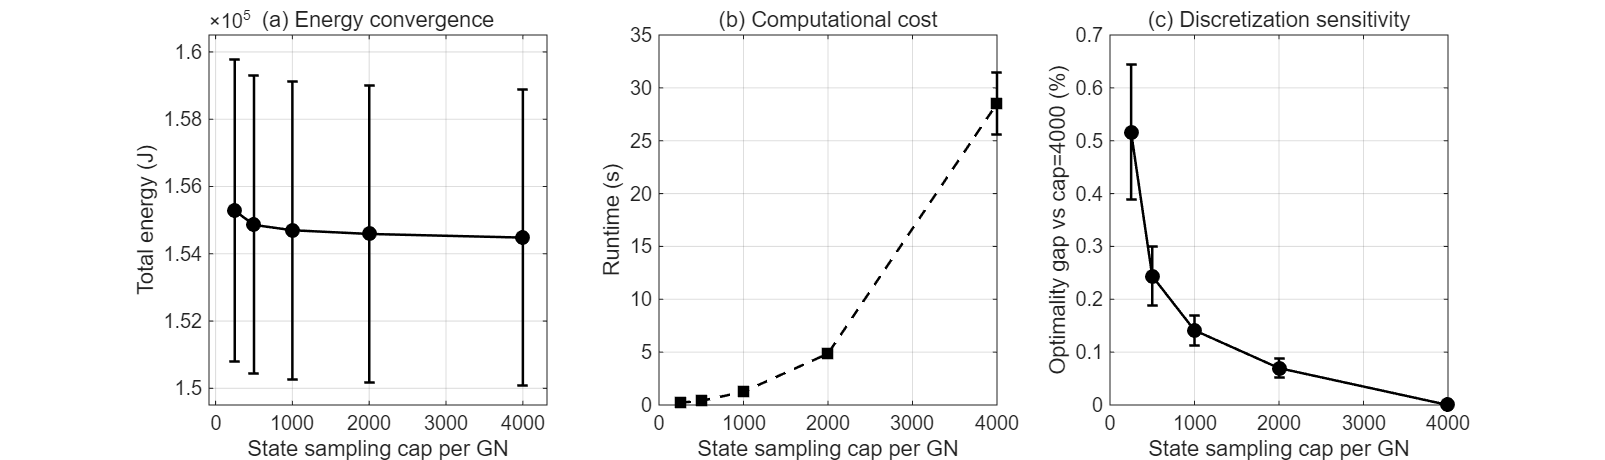
\includegraphics[width = 1\linewidth]{figures/discretization-sensitivity.png}
    \caption{Discretization sensitivity and computational cost. (a) Running time and (b) the relative optimality gap with respect to the finest resolution $M=4000$, versus the state sampling cap $M$. Each point is averaged over five random scenarios, with error bars denoting the standard deviation.}\label{fig:sensitivity}
\end{figure}

As shown in Table~\ref{tbl:sensitivity}, the total energy of every experiment decreases monotonically and converges as $M$ increases. On average, refining $M$ from $1000$ to $4000$ reduces the total energy by only $0.14\%$, and the improvement shrinks as the resolution doubles, indicating approximately first-order convergence (Fig.~(\ref{fig:sensitivity})(b)). At the operating resolution $M=2000$, the optimal energy is within $0.07\%$ of that obtained at $M=4000$; this residual gap reflects the discretization error of the state space and is negligible in practice, confirming that the discretized optimum has essentially converged to the continuous optimum. Meanwhile, as shown in Fig.~(\ref{fig:sensitivity})(a), the running time grows with $M$, averaging $4.86$ s at the operating resolution $M=2000$. Overall, a sampling cap in the range $M \in [1000, 2000]$ strikes a good balance between energy optimality and computational cost. Notably, even the coarsest resolution $M=250$ is only about $0.5\%$ above the finest $M=4000$, confirming that the discretization resolution has only a marginal impact on the optimal energy and mainly affects the computational cost.

\subsection{Real World Scenario Case Study}

\begin{figure}%[]
  \centering
   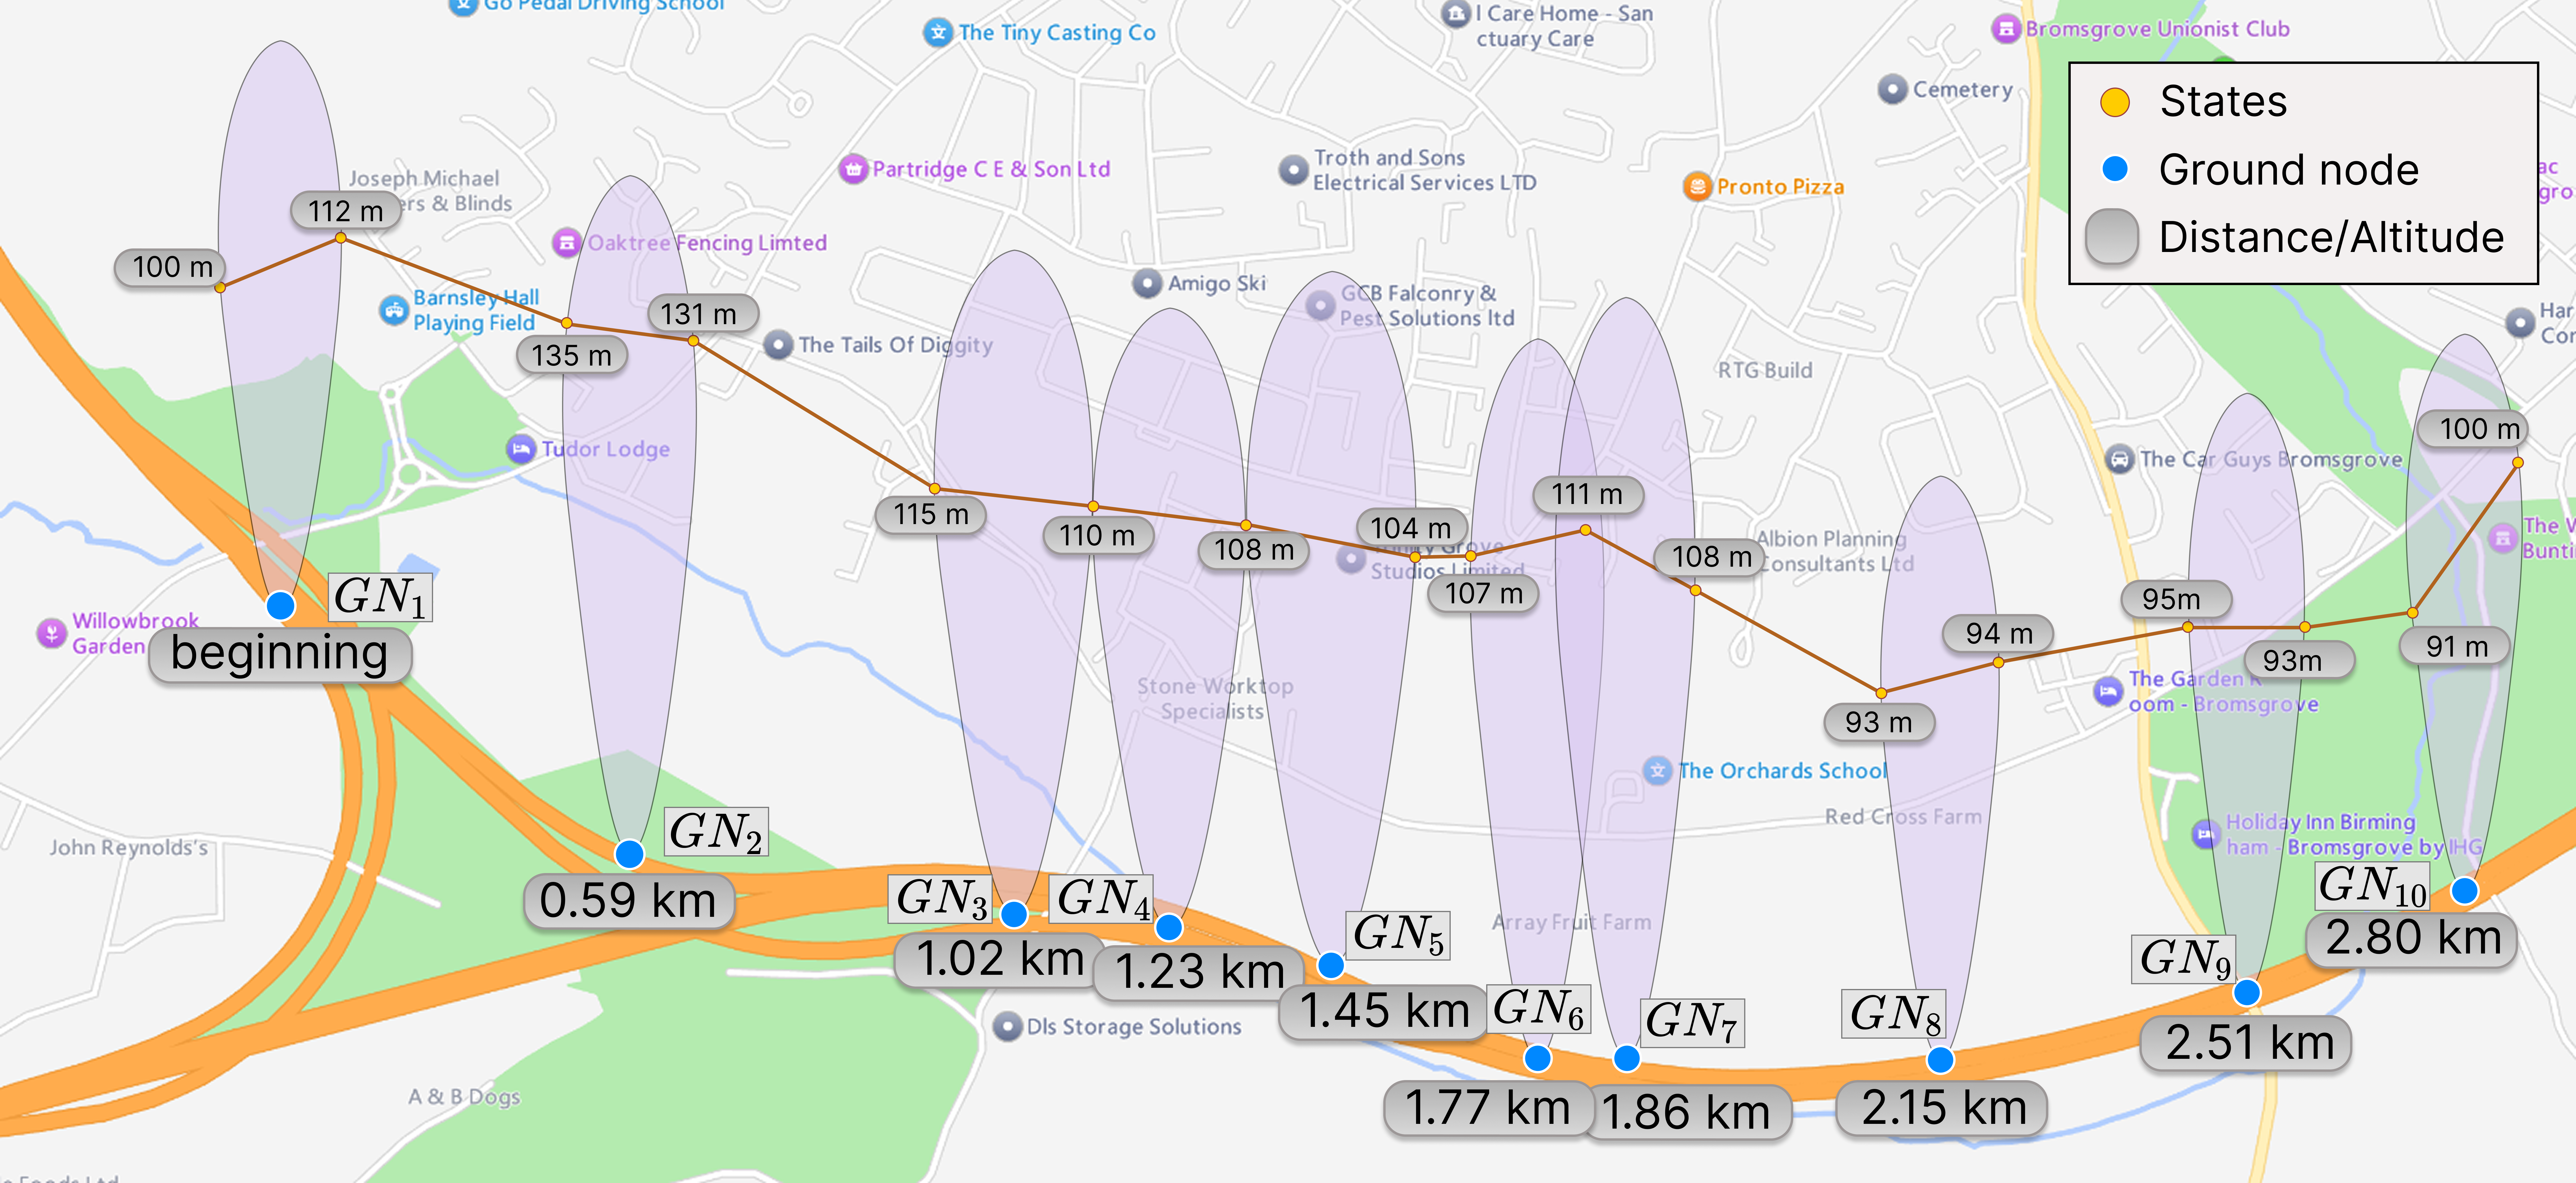
\includegraphics[width = 1\linewidth]{figures/real-world-scenario.png}
    \caption{The traffic CCTVs at M5, Bromsgrove, England, United Kingdom~\cite{UKLiveCamera}}\label{fig:real_scenario}
\end{figure}

\begin{table}%[]
\caption{Per-segment speed schedule of the \textit{JHVSO}-planned trajectory in the real-world scenario.}\label{tbl2}
\begin{tabular*}{\tblwidth}{lcccr}
\toprule
 Segment & Type & $v_\parallel (m/s)$ & $v_\perp$ & Duration (s) \\ % Table header row
\midrule
$GN_1$ & Task  & 7.00  & 0.57  & 21.00\\
$GN_2$ & Gap   & 13.94 & 0.80  & 28.76\\
$GN_2$ & Task  & 12.17 & -0.17 & 18.00\\
$GN_3$ & Gap   & 13.94 & -1.16 & 14.70\\
$GN_3$ & Task  & 11.40 & -0.25 & 20.00\\
$GN_4$ & Task(direct)  & 8.86  & -0.09 & 22.00\\
$GN_5$ & Task(direct)  & 12.89 & -0.21 & 19.00\\
$GN_6$ & Gap   & 13.96 & 0.38  & 7.81 \\
$GN_6$ & Task  & 8.94  & 0.24  & 17.00 \\
$GN_7$ & Task(direct)  & 9.17  & -0.25 & 12.00 \\
$GN_8$ & Gap   & 13.92 & -1.63 & 9.20 \\
$GN_8$ & Task  & 7.09  & 0.05  & 22.00 \\
$GN_9$ & Gap   & 13.96 & 0.07  & 14.54 \\
$GN_9$ & Task  & 7.18  & -0.09 & 22.00 \\
$GN_{10}$ & Gap   & 13.96 & -0.20 & 10.10 \\
$GN_{10}$ & Task  & 6.95  & 0.47 & 19.00 \\
\bottomrule
\end{tabular*}
\end{table}

We conduct a simulation using the real-world dataset, contains 10 public traffic CCTV cameras places at high way in Deciduous Broadleaf, England ,United Kingdom.
We assume that the UAV is deployed to collect data from these cameras.
Then by using our proposed \textit{JHVSO} algorithm, we scheduled the speed and altitude use for the mission , the UAV is constrained to start the mission at an altitude of 100 m at the first GN (i.e., $h_{0} = 100m$ in \textit{Definition. \ref{def:JHVSO}}), and the trajectory terminates at an altitude of 100 m within the communication region of the last GN.

\textit{Table. \ref{tbl2}} details the speed schedule of the planned trajectory on a per-segment basis.
In the Gap segments, the UAV cruises at horizontal speeds of $13.92-13.96 m/s$ with small vertical components bounded within $\pm 1.63 m/s$, and the segment durations range from $7.81 s$ to $28.76 s$, varying with the spacing between the coverage regions of adjacent GNs.
In the Task segments, the UAV slows down to $6.95-12.89 m/s$, and the duration of each Task segment equals the required collection time of the corresponding GN.
Notably, the transitions toward $GN_5$ and $GN_7$ contain no Gap segment, as the UAV has not yet left the communication coverage of the next GN upon finishing the previous collection task.
Overall, the mission is completed in $278 s$, of which $85.1 s\ (\approx30 \%)$ is spent on inter-node cruising.



%%%%%%%%%%%%%%%%%%%%%%%%%%%%%%%%%%%%%%%%%%%%%%%%%%%%%%%%%%%%%%%%%%%%%%%%%%%%%%%%%%
%%%%%%%%%%%%%%%%%%%%%%%%%%%%%%%%%%%%%%%%%%%%%%%%%%%%%%%%%%%%%%%%%%%%%%%%%%%%%%%%%%

 \section{Conclusion}
\label{sec:conclusion}

This paper studied energy-efficient three-dimensional speed scheduling for UAV data collection from sequentially ordered ground nodes.
Departing from prior formulations that either fix the flight altitude or treat altitude changes as discrete transitions between horizontal segments, we formulated the joint horizontal-vertical speed optimization (\textit{JHVSO}) problem, in which the UAV's horizontal and vertical velocity components are scheduled jointly and continuously, the ground-to-air communication range varies with the flight altitude, and each ground node imposes its own minimum data collection duration.

The solution of the \textit{JHVSO} problem was built on a sequence of analytical results.
Exploiting the strict convexity of the horizontal and vertical power components, we proved that constant-velocity straight-line flight is the unique energy minimizer between any two states under a fixed duration, and derived the pitch-angle-dependent speed that minimizes the energy consumption per unit distance when the flight duration is unconstrained.
We further established the non-aftereffect property of the multi-stage state transitions, which legitimizes a dynamic programming formulation.
Building on these results, the proposed Optimal Reached Energy (ORE) algorithm decomposes each inter-node transition into gap and task segments, evaluates feasible transitions through the communication-boundary entry states, and computes the global energy-optimal trajectory over the discretized state space; an exact algebraic restructuring of the recurrence reduces the per-stage complexity from $O(m \times j \times n)$ to $O(m \times j + j \times n)$ without sacrificing optimality. A sensitivity study further confirms that the discretized optimum converges to the continuous optimum with negligible loss (within $0.07\%$ at the operating resolution).

Extensive simulations under varying channel conditions, collection durations, node densities, and inter-node distances show that \textit{JHVSO} consistently consumes less energy than ASSUME, MSMO, ACO, and a greedy speed-height baseline, with an energy reduction of up to approximately $16.8\%$ over the greedy speed–height baseline and by up to 5.8\% over the strongest competing baseline.
A case study based on real-world traffic-camera locations further illustrates the practical trajectory patterns produced by ORE, in which the UAV cruises near its maximum-range speed along gap segments and adapts both its speed and altitude to the collection requirement and coverage geometry of each ground node.

Overall, by jointly scheduling the horizontal and vertical speed components together with the flight altitude, the proposed JHVSO framework delivers a rigorous, globally optimal, and computationally efficient solution to energy-minimal UAV data collection, reconciling the aerodynamic flight power model with the altitude-dependent communication coverage.


% Numbered list
% Use the style of numbering in square brackets.
% If nothing is used, default style will be taken.
%\begin{enumerate}[a)]
%\item 
%\item 
%\item 
%\end{enumerate}  

% Unnumbered list
%\begin{itemize}
%\item 
%\item 
%\item 
%\end{itemize}  

% Description list
%\begin{description}
%\item[]
%\item[] 
%\item[] 
%\end{description}  

% \clearpage %%Remove this from your manuscript

% Figure
% \begin{figure}%[]
%   \centering
% %    \includegraphics{}
%     \caption{}\label{fig1}
% \end{figure}


% \begin{table}%[]
% \caption{}\label{tbl1}
% \begin{tabular*}{\tblwidth}{@{}LL@{}}
% \toprule
%   &  \\ % Table header row
% \midrule
%  & \\
%  & \\
%  & \\
%  & \\
% \bottomrule
% \end{tabular*}
% \end{table}

% Uncomment and use as the case may be
%\begin{theorem} 
%\end{theorem}

% Uncomment and use as the case may be
%\begin{lemma} 
%\end{lemma}

%%%%%%%%%%%%%%%%%%%%%%%%%%%%%%%%%%%%%%%%%%%%%%%%%%%%%%%%%%%%%%%%%%%%%%%%%%%%%%%%%%
%%%%%%%%%%%%%%%%%%%%%%%%%%%%%%%%%%%%%%%%%%%%%%%%%%%%%%%%%%%%%%%%%%%%%%%%%%%%%%%%%%

%% The Appendices part is started with the command \appendix;
%% appendix sections are then done as normal sections

\appendix
\section*{Appendix}
\section{\textit{Proof of Lemma~\ref{lem:ver}}}
\label{pro:Lemma ver}

Write Eq.~(\ref{equ:v_1}) as $P_\perp(v) = k_1mg[v/2 + \sqrt{(v^2/4 + c)}] + c_1(mg)^{3/2}$ with the shorthand $c = mg/k_2^2 > 0$ and $v = V_\perp$.
Differentiating twice, the linear term $v/2$ vanishes, the constant profile-power term $c_1(mg)^{3/2} $vanishes, and the square-root term yields

    \[ P_\perp ''(v) = k_1mg \cdot c / (4(v^2/4 + c)^{3/2}) \]

    Since $k_1$, $mg$, and $c$ are all positive, the numerator is strictly positive and the denominator is strictly positive and finite for every $v \in \mathbb{R} $.
    Hence $P_\perp''(v) > 0$ everywhere, and $P_\perp$ is strictly convex on $\mathbb{R}$.
    \qed

\section{\textit{Proof of Lemma~\ref{lem:hor}}}
\label{pro:Lemma hor}
The hovering power $P_{mh}$ is constant and does not affect the curvature.
The profile and parasite terms contribute $2c_2 > 0$ and $6c_1v \geq 0$ to the second derivative, respectively, and are therefore (strictly) convex on $v \geq 0$.
The only non-trivial part is the induced-power increment.
Substituting $u = v^2/(2v_0^2) \geq 0$ and differentiating twice gives, after simplification, the closed form

    \[ f''(v) = (1/(2v_0^2)) \cdot \phi(u),\]
    \[ \phi(u) = \frac{(2u - \sqrt{(1+u^2)}) \cdot \sqrt{(\sqrt{(1+u^2)} + u)} }{ (1+u^2)^{3/2}} \]

    The factor $\phi(u)$ vanishes at $u = 1/\sqrt{3}$ (equivalently, at $v = (2/3)^{1/4}v_0$), is positive beyond it, and is negative before it; hence the induced-power increment alone is concave near the origin, which is precisely the mathematical trace of the well-known effect that moderate forward flight relieves the induced drag.
    However, direct evaluation of the closed form shows that $\phi$ attains its global minimum at $u = 0$ with $\phi(0) = -1$, so $f''(v) \geq -1/(2v_0^2)$ for all $v \geq 0$, with equality only at $v = 0$.
    Combining all four terms,

    \begin{eqnarray*}
        P_\parallel''(v)  & = & 2c_2 + 6c_1v + P_{in}\cdot f''(v) \\ 
                    & \geq & 2c_2 - P_{in}/(2v_0^2) + 6c_1v\\ 
                    & \geq & 2c_2 - P_{in}/(2v_0^2)\\ 
                        & > & 0 
    \end{eqnarray*}

    where the last inequality follows from $4c_2v_0^2 > P_{in}$.
    Thus $P_\parallel$ is strictly convex on $v \geq 0$. 

    % \[P_\parallel''(v) = 2c_2 + 6c_1v + P_{in}\cdot f''(v) \geq\]
    %  \[2c_2 - P_{in}/(2v_0^2) + 6c_1v \geq\]
    %   \[2c_2 - P_{in}/(2v_0^2) > 0,\]

    It remains to argue that the condition $4c_2v_0^2 > P_{in}$ is not restrictive.
    First, substituting the expressions of $c_2, P_{in}$, and the momentum-theory identity $v_0^2 = W/(2n\rho A)$, the condition reduces to $(3\delta s)/(4\sqrt{C_T}) > (1+k)/\sqrt{2}$, which involves only the dimensionless aerodynamic constants of the rotor blades and is independent of the platform weight, rotor number, and disc area.
    Second, evaluated with the representative parameter set reported in~\cite{GongHao} $(W = 20 N, n = 4, \rho = 1.168 kg/m^3, A = 0.214 m^2, \delta = 0.011, s = 0.045, C_T = 0.001195, v_0 = 6.325 m/s, k = 0.11)$, the two sides evaluate to $4c_2v_0^2 \approx 111.1 W$ and $P_{in} \approx 70.2 W$, and the condition holds.
    Third, even if the condition were violated for an unconventional configuration, strict convexity would fail only in a neighbourhood of the origin: since $f''(v) \rightarrow  0$ as $v \rightarrow \infty $ while the parasite term $6c_1v$ grows linearly, there always exists a speed threshold beyond which $P_\parallel ''(v) > 0$; the non-convex region, if any, is confined to low speeds that are dominated by the hovering regime and are of limited practical interest for cruise scheduling.
    \qed

\section{\textit{Proof of Theorem~\ref{thm:optimal-range-speed}}}

\label{pro:Theorem optimal-range-speed}

Let $\mathcal{E}(d) = L \cdot LUT(\gamma)$ define the energy consumption function for a spatial displacement vector $d = (L \cos\gamma, L \sin\gamma)^T$.
Consider the energy consumption as a function of the displacement in a 2D vertical flight plane $d = (x, y)^T$, where $x = L \cos\gamma$ and $y = L \sin\gamma$.
The norm of the displacement is $r = L = \sqrt{x^2 + y^2}$ and the pitch angle is $\gamma = \arctan(y/x)$.
We define the energy functional as:

$$\mathcal{E}(x,y) = \sqrt{x^2 + y^2} \cdot LUT\left(\arctan\left(\frac{y}{x}\right)\right)$$

To establish that $\mathcal{E}(x,y)$ is convex, we examine its Hessian matrix $H$.
Let $f(\gamma) = LUT(\gamma)$.
By applying the chain rule, the first-order partial derivatives of the polar variables with respect to the Cartesian coordinates are:

$$\frac{\partial r}{\partial x} = \cos\gamma, \quad \frac{\partial r}{\partial y} = \sin\gamma, \quad \frac{\partial \gamma}{\partial x} = -\frac{\sin\gamma}{r}, \quad \frac{\partial \gamma}{\partial y} = \frac{\cos\gamma}{r}$$

The first-order partial derivatives of the energy functional $\mathcal{E} = r \cdot f(\gamma)$ are:

$$\mathcal{E}_x = \frac{\partial}{\partial x}[r f(\gamma)] = f(\gamma)\cos\gamma - f'(\gamma)\sin\gamma$$

$$\mathcal{E}_y = \frac{\partial}{\partial y}[r f(\gamma)] = f(\gamma)\sin\gamma + f'(\gamma)\cos\gamma$$

Taking the partial derivatives again to construct the Hessian matrix $H = \begin{pmatrix} \mathcal{E}_{xx} & \mathcal{E}_{xy} \\ \mathcal{E}_{yx} & \mathcal{E}_{yy} \end{pmatrix}$, we obtain:

$$\mathcal{E}_{xx} = \frac{\partial \mathcal{E}_x}{\partial \gamma}\frac{\partial \gamma}{\partial x} = -(f(\gamma) + f''(\gamma))\sin\gamma \left(-\frac{\sin\gamma}{r}\right) $$

\[= \frac{\sin^2\gamma}{r}(f(\gamma) + f''(\gamma))\]

$$\mathcal{E}_{yy} = \frac{\partial \mathcal{E}_y}{\partial \gamma}\frac{\partial \gamma}{\partial y} = (f(\gamma) + f''(\gamma))\cos\gamma \left(\frac{\cos\gamma}{r}\right) $$

\[= \frac{\cos^2\gamma}{r}(f(\gamma) + f''(\gamma))\]

$$\mathcal{E}_{xy} = \frac{\partial \mathcal{E}_x}{\partial \gamma}\frac{\partial \gamma}{\partial y} = -(f(\gamma) + f''(\gamma))\sin\gamma \left(\frac{\cos\gamma}{r}\right) $$

\[= -\frac{\sin\gamma\cos\gamma}{r}(f(\gamma) + f''(\gamma))\]

Factoring out the common terms, the Hessian matrix can be elegantly expressed as:

$$H = \frac{f(\gamma) + f''(\gamma)}{r} \begin{pmatrix} \sin^2\gamma & -\sin\gamma\cos\gamma \\ -\sin\gamma\cos\gamma & \cos^2\gamma \end{pmatrix}$$

To determine the convexity, we analyse the eigenvalues of the angular matrix $M = \begin{pmatrix} \sin^2\gamma & -\sin\gamma\cos\gamma \\ -\sin\gamma\cos\gamma & \cos^2\gamma \end{pmatrix}$.
The trace of $M$ is $Tr(M) = \sin^2\gamma + \cos^2\gamma = 1$, and its determinant is $Det(M) = \sin^2\gamma\cos^2\gamma - (-\sin\gamma\cos\gamma)^2 = 0$.
Consequently, the eigenvalues of $M$ are $0$ and $1$, which yields the eigenvalues of the full Hessian matrix $H$:

$$\lambda_1 = 0, \quad \lambda_2 = \frac{f(\gamma) + f''(\gamma)}{r}$$

The zero eigenvalue $\lambda_1$ corresponds to the radial direction, reflecting the linear scaling of energy with distance along a straight line (no curvature).
For the energy functional to be strictly convex in all tangential directions (ensuring that any angular deviation or detour incurs a strict energy penalty), the non-zero eigenvalue $\lambda_2$ must be strictly positive.
Since $r > 0$, this yields the fundamental requirement:

\begin{figure}%[]
  \centering
   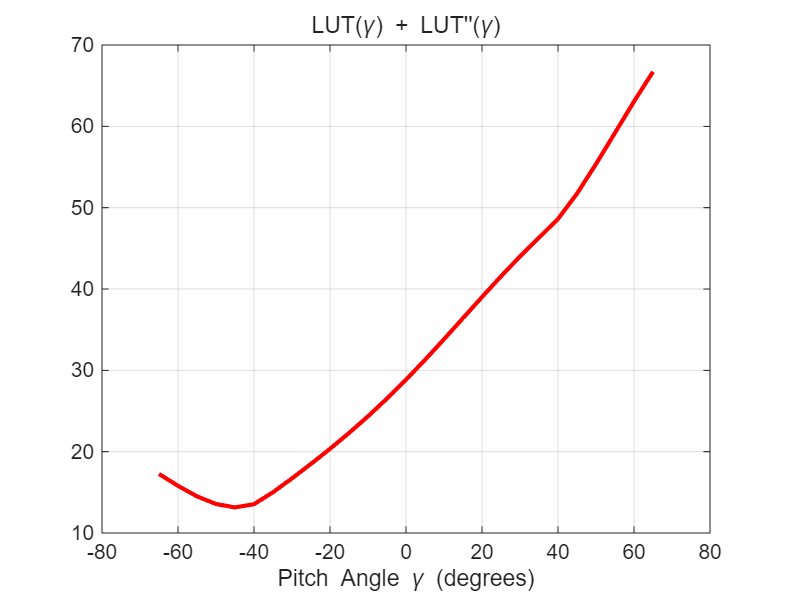
\includegraphics[width = 0.8\linewidth]{figures/lut-transition-comparison.png}
    \caption{ Shows that $LUT(\gamma)+LUT''(\gamma)$ above 0 for all pitch angles }\label{fig:LUT'+LUT''}
\end{figure}

$$f(\gamma) + f''(\gamma) > 0$$

Given that $LUT(\gamma)$ represents the optimal unit-distance energy cost, it is physically constrained to be positive, $LUT(\gamma) > 0$.
For $\mathcal{E}$ to be convex in all tangential directions, it suffices that $f(\gamma)'+f(\gamma)''>0$, which is numerically verified over the operational pitch-angle domain (Fig.~(\ref{fig:LUT'+LUT''})); for other platforms this condition can be checked offline once the LUT is constructed.

This rigorous matrix analysis confirms that the energy functional $\mathcal{E}(x,y)$ defines a strictly convex metric in the spatial field.
To bridge the theoretical gap between the strict convexity of the energy functional $\mathcal{E}(d)$ and its sub-additivity ($\mathcal{E}(d_1+d_2)<\mathcal{E}(d_1)+\mathcal{E}(d_2)$), we must first establish its positive 1-homogeneity.
For any spatial displacement vector $d$ and any positive scalar $\alpha > 0$, scaling the flight distance by $\alpha$ while maintaining the same pitch angle scales the total energy linearly.
Mathematically, this is expressed as $\mathcal{E}(\alpha d) = \|\alpha d\| \cdot LUT(\gamma) = \alpha \|d\| \cdot LUT(\gamma) = \alpha \mathcal{E}(d)$.

With both strict convexity and positive 1-homogeneity established, we can mathematically prove the strict sub-additivity for any two non-collinear displacement vectors $d_1$ and $d_2$.
Let $S = \mathcal{E}(d_1) + \mathcal{E}(d_2)$ represent the combined energy of the two independent segments.
We construct two energy-normalized vectors, $\tilde{d}_1 = \frac{d_1}{\mathcal{E}(d_1)}$ and $\tilde{d}_2 = \frac{d_2}{\mathcal{E}(d_2)}$.
Due to the 1-homogeneity, the energy of these normalized vectors is exactly unity, such that $\mathcal{E}(\tilde{d}_1) = \mathcal{E}(\tilde{d}_2) = 1$.

We define a convex combination parameter $\lambda = \frac{\mathcal{E}(d_1)}{S}$, which logically ensures $1 - \lambda = \frac{\mathcal{E}(d_2)}{S}$ and bounds the parameter within $\lambda \in (0, 1)$.
Applying the strict convexity property to these normalized vectors yields the inequality $\mathcal{E}(\lambda \tilde{d}_1 + (1-\lambda)\tilde{d}_2) < \lambda \mathcal{E}(\tilde{d}_1) + (1-\lambda)\mathcal{E}(\tilde{d}_2)$.

Substituting the definitions of $\lambda$, $\tilde{d}_1$, and $\tilde{d}_2$ into the left side of the inequality results in $\mathcal{E}\left(\frac{d_1 + d_2}{S}\right)$.
By extracting the scalar fraction $1/S$ using the 1-homogeneity property, the left side simplifies to $\frac{1}{S}\mathcal{E}(d_1 + d_2)$.
Concurrently, evaluating the right side yields $\lambda(1) + (1-\lambda)(1) = 1$.
Combining both sides produces $\frac{1}{S}\mathcal{E}(d_1 + d_2) < 1$.

Multiplying the entire expression by $S$ directly establishes the strict sub-additivity property: $\mathcal{E}(d_1 + d_2) < \mathcal{E}(d_1) + \mathcal{E}(d_2)$.
This mathematically proves that within this strictly convex spatial field, the energy required to traverse the vector sum of two non-collinear segments is strictly less than the sum of the energies required to traverse them individually.

Extending this foundational property to the continuous UAV trajectory problem, any detour path connecting the start and end points can be discretized into a sequence of $n$ spatial vectors such that $\sum_{i=1}^{n} d_i = d_{direct}$.
If at least one segment deviates from the direct geometric baseline (meaning the segments are not positively collinear), the strict sub-additivity iteratively dictates that the total energy cost of the detour strictly exceeds the direct path energy:

$$\sum_{i=1}^{n}\mathcal{E}(d_i) > \mathcal{E}\left(\sum_{i=1}^{n}d_i\right) = \mathcal{E}(d_{direct})$$

Thus, the direct straight-line path is mathematically proven to be the unique global energy minimizer.
This approach comprehensively resolves the transition optimality of gap segment by treating the energy cost as a cohesive spatial field governed by the positive definiteness of the Hessian matrix.
\qed

%%%%%%%%%%%%%%%%%%%%%%%%%%%%%%%%%%%%%%%%%%%%%%%%%%%%%%%%%%%%%%%%%%%%%%%%%%%%%%%%%%
%%%%%%%%%%%%%%%%%%%%%%%%%%%%%%%%%%%%%%%%%%%%%%%%%%%%%%%%%%%%%%%%%%%%%%%%%%%%%%%%%%


% To print the credit authorship contribution details
\printcredits

%% Loading bibliography style file
\bibliographystyle{ieeetr}

% Loading bibliography database
\bibliography{references}

% Biography
%\bio{}
% Here goes the biography details.
%\endbio

%\bio{pic1}
% Here goes the biography details.
%\endbio

\end{document}
